% concatenated from main.tex
\documentclass[11pt]{amsart}
\usepackage{fullpage}
\usepackage{amsfonts,amssymb,amsmath,amsthm}
\usepackage{hyperref}
\usepackage{color}
\usepackage{comment}
\usepackage{tikz-cd}      
\usepackage[backend=biber]{biblatex}
\addbibresource{references.bib}
\DeclareFieldFormat{doi}{} %
\DeclareFieldFormat{isbn}{}  %
\DeclareFieldFormat{issn}{} %
\DeclareFieldFormat{url}{} %
\DeclareFieldFormat{urldate}{} %

\DeclareMathOperator{\sgn}{sgn}
\theoremstyle{plain}
\newtheorem{theorem}{Theorem}[section]
\newtheorem*{theorem*}{Theorem}
 \newtheorem{corollary}[theorem]{Corollary}
 \newtheorem{conjecture}[theorem]{Conjecture}
 \newtheorem{lemma}[theorem]{Lemma}
 \newtheorem{proposition}[theorem]{Proposition}
 \theoremstyle{definition}
 \newtheorem{definition}[theorem]{Definition}
 \newtheorem{setting}[theorem]{Setting}
 \theoremstyle{remark}
 \newtheorem{remark}[theorem]{Remark}
 \numberwithin{equation}{section}
  \newtheorem{example}[theorem]{Example}
 \newtheorem{exercise}[theorem]{Exercise}

\newcommand{\SF}[1]{  [SF: #1]}
\def\fz{\mathfrak{z}}
\def\fg{\mathfrak{g}}
\def\fv{\mathfrak{v}}

\def\cA{\mathcal{A}}
\def\cB{\mathcal{B}}
\def\cE{\mathcal{E}}
\def\cK{\mathcal{K}}
\def\cN{\mathcal{N}}
\def\cJ{\mathcal{J}}
\def\cU{\mathcal{U}}
\def\cG{\mathcal{G}}
\def\cD{\mathcal{D}}
\def\0s{\setminus\{0\}}
\def\cI{\mathcal{I}}
\def\cH{\mathcal{H}}
\def\cF{\mathcal{F}}
\def\cL{\mathcal{L}}
\def\ddt{\frac{d}{dt}\big|_{t=0}}

\def\vol{{\rm vol}}
\def\CP{\mathbb{CP}}

\def\mz{\setminus\{0\}}


\def\eps{\varepsilon}
\def\R{{\mathbb R}}%
\def\C{{\mathbb C}}%
\def\N{{\mathbb N}}%
\def\Z{{\mathbb Z}}%
\def\T{{\mathbb T}}%
\mathchardef\mhyphen="2D %
\def \PD { {\rm P\!\mhyphen \!\rm D} } %
\def \pd { {{\mathfrak p}\mhyphen {\mathfrak d}}}
\def \PM { {\rm P\!\mhyphen \!\rm M} } %
\def \ad {{\rm ad}}
\def \expX{\exp^\mathbf{X}}
\def \expY{\exp^\mathbf{Y}}
\def \lnX{\ln^\mathbf{X}}
\def \lnY{\ln^\mathbf{Y}}
\def \LnX{{\rm Ln}^\mathbf{X}}
\def \LnY{{\rm Ln}^\mathbf{Y}}
\def \Exp {{\rm Exp}}
\def \Ln{{\rm Ln}}
\def \ExpX{{\rm Exp}^\mathbf{X}}
\def \ExpY{{\rm Exp}^\mathbf{Y}}
\def\Op{{\rm Op}}
\def\expf{\mathfrak{exp}}
\def \Ghat{\widehat{G}}
\def \Hhat{\widehat{H}}
\def \PullOne{\mathcal{I}_\Phi}
\def \PullTwo{\mathcal{U}_\Phi}
\def \pr {{\rm pr}} %
\def \jac {{\rm jac}}
\def \supp {{\rm supp}}
\def \diag{{\rm diag}}
\def \heis {\mathbb{H}}
\def\osc{{\rm osc}}

\newcommand{\tr}[1]{{\rm tr}\left(#1\right)}

\def\Tend#1#2{\mathop{\longrightarrow}\limits_{#1\rightarrow#2}}

\newcommand{\kernelSpace}[1]{\Gamma_c\left(\mathcal{S}(#1, |\Lambda|\mathcal{V})\right)}

\numberwithin{equation}{section}

\begin{document}
	\title[The sub-Riemannian X-ray transform on $H$-type groups]{The sub-Riemannian X-ray transform on $H$-type groups: Fourier slice theorems, injectivity sets and frequency support}

	\author[S. Flynn]{Steven Flynn}
	\address[S. Flynn]{Department of Mathematics, University College London, Gower Street, London WC1E 6BT, United Kingdom}
	\email{steven.flynn@ucl.ac.uk}
	\subjclass[2020]{44A12, 53C17, 43A80, 22E30, 35R30}
	\keywords{X-ray transform, sub-Riemannian geometry, $H$-type groups, group Fourier transform, conjugate points, limited-data tomography}


\begin{abstract}
	We study the X-ray transform along sub-Riemannian geodesics of $H$-type groups, a setting in which every geodesic apart from the horizontal lines carries conjugate points. The geodesics are helices labelled by a charge $\lambda$ in the dual of the center. Using the group Fourier transform we prove a Fourier slice theorem, which identifies the transform restricted to the geodesics of charge $\lambda$ as a Fourier restriction to their visible frequencies $\Gamma_\lambda^*$, a family of parallel hyperplanes of central frequencies dual to the central advance of the helices, followed by an explicit operator-valued multiplier. We characterize the sets of charges $Z$ whose geodesics determine an integrable function, one direction for each $\lambda\in Z$ sufficing, as exactly those for which $\bigcup_{\lambda\in Z}\Gamma_\lambda^*$ is dense. In particular the full transform is injective, and when the center has dimension at least two, charges of a single magnitude suffice provided their directions fill a circle. Averaging the normal operator over the horizontal directions gives a joint spectral multiplier of the sub-Laplacian and the central derivatives, whose eigenvalues we compute. This yields, outside the first Heisenberg group, a sharp stability estimate at fixed charge and central frequency with the loss of exactly half a derivative in the sub-Laplacian, as for the Euclidean X-ray transform. Finally we describe which central frequencies of $f$ are determined by a band or a cap of charges, namely all sufficiently high ones, the bounded remainder being recovered only by analytic continuation, in contrast with Euclidean limited-angle tomography.
\end{abstract}

\maketitle

\makeatletter
\renewcommand\l@subsection{\@tocline{2}{0pt}{3pc}{5pc}{}}
\makeatother


\tableofcontents


\section{Introduction}

Let $G$ be an $H$-type group (defined in Section \ref{H-type}) with its left-invariant sub-Riemannian metric, and let $\cG$ be the set of maximal oriented sub-Riemannian geodesics in $G$. The \textit{X-ray transform} of a function $f$ on $G$ is
\begin{align*}
	I(f)(\gamma):=\int_\gamma f\, ds, \quad \gamma\in \cG.
\end{align*}
This paper asks which subfamilies of $\cG$ determine $f$, and how stably. 

Geodesic X-ray transforms are extensively studied in Riemannian geometry \cite{sharafutdinovIntegralGeometryTensor1994, ilmavirtaIntegralGeometryManifolds2018, paternainGeometricInverseProblems2023}, because of their application to noninvasive imaging \cite{nattererMathematicsComputerizedTomography1986} and because they are the linearizations of the boundary and spectral rigidity problems \cite{stefanovRigidityMetricsSame1998, guilleminInverseSpectralResults1980}, and on groups and symmetric spaces with a left-invariant Riemannian metric \cite{helgasonIntegralGeometryRadon2011, ilmavirtaRadonTransformsCompact2016, ilmavirtaTorusComputedTomography2020a, kleinFunkTransformCompact2009}.

Tomographic data are often restricted to a subfamily of lines, by the imaging apparatus or by the geometry \cite{gelfandDifferentialFormsIntegral1969, greenleafNonlocalInversionFormulas1989}. When the admissible curves are those tangent to a distribution $\cD\subset TM$, two cases arise. If $\cD$ is integrable the transform is a family of leafwise problems, as in single-axis tilt electron tomography \cite{quintoLocalTomographyElectron2008} or parallel-beam computed tomography \cite{nattererMathematicsComputerizedTomography1986}. If $\cD$ is bracket generating there is no such reduction, and if $\cD$ carries a metric the horizontal curves of stationary energy are the \textit{sub-Riemannian geodesics}. The simplest case is the horizontal lines of the first Heisenberg group $\heis_1$, a three-parameter family of lines in $\R^3$, and the transform along them is not injective \cite{strichartzLpHarmonicAnalysis1991}. See also \cite{rubinRadonTransformHeisenberg2012, peyerimhoffXrayTransform2step2016} for Radon and X-ray transforms on two-step nilpotent groups. To the author's knowledge, X-ray tomography along sub-Riemannian geodesics is otherwise unexplored aside from \cite{flynnInjectivityHeisenbergXray2021, flynnSingularValueDecomposition2023}.


$H$-type groups, first introduced by Kaplan \cite{kaplanFundamentalSolutionsClass1980, kaplanRiemannianNilmanifoldsAttached1981}, are the model case for step-two sub-Riemannian geometry and the simplest class of nilpotent groups beyond the classical Heisenberg groups. The Iwasawa $N$-groups among them (Example \ref{ex:htype}) are the boundary at infinity, minus a point, of the rank one symmetric spaces of noncompact type \cite{follandHardySpacesHomogeneous1982b, cowlingHTypeGroupsLwasawa}, where the sub-Riemannian structure is the natural one induced on the boundary, and their nilmanifolds are sufficiently diverse to construct the first examples of closed isospectral Riemannian manifolds that are not locally isometric \cite{gordonIsospectralClosedRiemannian1993}.

The Lie algebra $\fg=T_eG$ of an $H$-type group has the vector space decomposition
\begin{align*}
	\fg=\fv\oplus \fz
\end{align*}
where $\fz\neq 0$ is the center of $\fg$ and $[\fv, \fv]=\fz$. The subspace $\fv$ determines a left-invariant \textit{horizontal} distribution $\cD_q:=dL_q(\fv)$, $q\in G$, which satisfies H\"{o}rmander's condition. Chow's theorem guarantees that $G$ is path connected by absolutely continuous curves whose derivatives are almost everywhere horizontal \cite{montgomeryTourSubriemannianGeometries2006}, that is, for which
\begin{align}\label{horizontal}
	\dot{\gamma}(t)\in \cD_{\gamma(t)} \quad \text{for} \quad t \text{ a.e.}
\end{align}
A sub-Riemannian geodesic is a horizontal curve that locally minimizes length, measured by the inner product on $\fv$, among horizontal curves with the same endpoints. Since $G$ has step two, every geodesic is normal \cite{montgomeryTourSubriemannianGeometries2006}, that is, the projection of a trajectory of the Hamiltonian flow of Section \ref{HamFormalism}, and $\cG$ is described completely by that flow.

On an $H$-type group the constraint \eqref{horizontal} reads $\Theta(\dot\gamma(t))=0$, where $\Theta$ is the left-invariant $\fz$-valued one-form which at the identity is the projection of $\fg$ onto $\fz$. Equivalently, $\Theta$ is a connection on the principal $\fz$-bundle $G\to G/\exp(\fz)\cong\fv$ whose curvature is the left-invariant $\fz$-valued two-form $\omega=d\Theta$ of \eqref{product}, and the geodesics are the horizontal lifts of the trajectories of a charged particle in $\fv$ moving in the constant generalized magnetic field $\omega$. The charge $\lambda\in \fz^*$, the vertical component of the generalized momenta,  is a constant of motion (Section \ref{sRGeometry}) and determines the Lorentz force $\omega_\lambda=\lambda\circ\omega$. The X-ray transform along magnetic geodesics is studied in \cite{dairbekovBoundaryRigidityMagnetic2007}, and for a constant field in $\R^3$ in \cite[Section 10.3]{stefanovGeodesicXrayTransform2012}. Here it appears, with an attenuation, as the family of central Fourier modes of $I$ (Remark \ref{r:twistedSlice}). 

Our results are organized by the charge. A geodesic with $\lambda\neq0$ is a helix of radius $|\lambda|^{-1}$ whose component in the center $\fz$ advances by $\pi|\lambda|^{-2}\hat\lambda$ per turn, and these advances generate the \textit{central lattice} $\Gamma_\lambda\subset\exp(\fz)$. Any such geodesic is a left translate of a model helix $\gamma_{\nu, \lambda}$ with horizontal momentum $\nu\in S(\fv^*)$, and the data split accordingly into the transforms $I_{\nu, \lambda}f(x, u):=\int_\R f((x, u)\gamma_{\nu, \lambda}(s))\,ds$, functions on a quotient of $G$ (Section \ref{spaceGeodesics}). A set of charges $Z\subset\fz^*\mz$ is an \textit{injectivity set} if $I_{\nu, \lambda}f=0$ for every $\lambda\in Z$, with $\nu$ allowed to depend on $\lambda$, forces $f=0$. The geodesics of charge $\lambda$ determine the group Fourier transform $\cF(f)(\mu)$ at the \textit{visible frequencies} $\mu\in \Gamma_\lambda^*$, the characters of the center trivial on $\Gamma_\lambda$, which form a family of parallel hyperplanes orthogonal to $\lambda$ with spacing $2|\lambda|^2$ (Theorem \ref{FourierSliceTheorem}).
\begin{theorem*}[Characterization of Injectivity Sets]
	A subset $Z\subset \fz^*\mz$ is an injectivity set of $I$ if and only if $\bigcup_{\lambda\in Z}\Gamma_\lambda^*$ is dense in $\fz^*$.
\end{theorem*}
This is Theorem \ref{MainResult}. A single direction at charge $\lambda$ already determines $\cF(f)(\mu)$ on $\lambda^\perp$ and on every other hyperplane of $\Gamma_\lambda^*$ (Theorem \ref{t:singleDirection}), and when $\dim\fz\geq2$ one can use charges of a single magnitude, provided their directions fill a circle in $S(\fz^*)$ (Corollary \ref{c:injSets}). By homogeneity any fixed magnitude serves (Proposition \ref{homogeneity}).

At a fixed charge we average the normal operator over the horizontal directions and compute its eigenvalues. For $n>1$, where $2n=\dim\fv$, the data from all directions at charge $\lambda$ determine $\cF(f)(\mu)$, $\mu\in \Gamma_\lambda^*$, with the loss of exactly half a derivative in the sub-Laplacian, as for the Euclidean X-ray transform \cite{strichartzLpEstimatesRadon1981} (Theorem \ref{t:stability}). The constants are explicit in $|\lambda|$, by scaling, and otherwise depend only on which hyperplane of $\Gamma_\lambda^*$ contains $\mu$ and on $|\mu|/|\lambda|^2$. They cannot be made uniform in these two parameters, since the estimate fails on the countable exceptional set of frequencies where the averaged normal operator has a kernel, and the uniform estimate away from that set, which a stability theorem for $I$ in norms on $G$ and $\cG$ would require, is left to a sequel.

The Heisenberg group $\heis_1$ was treated in \cite{flynnInjectivityHeisenbergXray2021}, where the Fourier slice theorem was proved and injectivity on $L^1(\heis_1)$ deduced from the geodesics of all charges in a neighborhood of zero. New here are the $H$-type groups of every dimension, on which the direction $\nu$ is a parameter (on $\heis_1$ all directions are rotations of one another) and, for $\dim\fz\geq2$, the charge and the central frequency need not be parallel. Also new are the characterization of the injectivity sets, the averaged normal operator with its eigenvalues and the stability estimate, and the visible frequencies of a band or cap of charges.

Conjugate points are a central obstacle in geometric inverse problems. They add to the normal operator a Fourier integral operator associated with the conjugate locus \cite{stefanovGeodesicXrayTransform2012}, inhibit stable inversion of the X-ray transform on Riemannian manifolds \cite{holmanAttenuatedGeodesicXray2018}, and force a loss in two dimensions \cite{monardGeodesicRayTransform2015}. On $H$-type groups they are ubiquitous. Along every geodesic $\gamma$ of charge $\lambda\neq 0$ the first conjugate point occurs at arclength $2\pi/|\lambda|$, and the conjugate points along $\gamma$ are the translates $\gamma(s+2\pi j|\lambda|^{-1})=(0, j\pi|\lambda|^{-2}\hat\lambda)\gamma(s)$, $j\in \Z$, an orbit of $\Gamma_\lambda$. The lattice $\Gamma_\lambda$ plays the role of the antipodal map on the sphere, where every great circle through $x$ passes through $-x$ (see \cite[Section 10.2]{stefanovGeodesicXrayTransform2012}). Nonetheless $I$ is injective on $L^1(G)$ for every $H$-type group. The periodicity of the conjugate points is what makes the spectrum of the transform computable. Since $I_{\nu, \lambda}f$ is unchanged when $f$ is translated by $\Gamma_\lambda$, the fixed-charge transform factors through $G/\Gamma_\lambda$, and the only frequencies of $f$ that can be recovered are those with $\mu\in \Gamma_\lambda^*$, which respect the quotient. Theorem \ref{MainResult} says that this is the only obstruction.

Our methods rest on the unitary representation theory of $H$-type groups, in the same way that the Euclidean theory of the X-ray and Radon transforms rests on the classical Fourier transform \cite{helgasonIntegralGeometryRadon2011}. In the Riemannian setting the stability of the X-ray transform is read off from the fact that the normal operator $I^*I$ is an elliptic pseudodifferential operator of order $-1$ \cite{stefanovBoundaryRigidityStability2005a}, a statement which fails in the presence of conjugate points \cite{stefanovGeodesicXrayTransform2012, monardGeodesicRayTransform2015, holmanAttenuatedGeodesicXray2018}. On a graded nilpotent group the left-invariant pseudodifferential operators of the calculus of \cite{fischerQuantizationNilpotentLie2016} are Fourier multipliers, and this is the form our results take. The Fourier slice theorem identifies the X-ray transform at fixed charge and direction as a left-invariant operator from $G$ to $G/\Gamma_\lambda$ with operator-valued symbol. The full normal operator $I^*I$ is not defined with the Lebesgue measure on charges. A geodesic of charge $\lambda$ spends length of order $|\lambda|$ in any fixed neighborhood of a point, so the integral over $\fz^*$ that defines its kernel diverges. Averaging over the directions at a fixed $\lambda$ instead produces a normal operator $\cN_\lambda$ which is a joint spectral multiplier of the sub-Laplacian $\Delta_{\rm{sr}}=\sum_j X_j^2$ and the central derivatives. On each central frequency $\mu$ it agrees to leading order in the spectral parameter with $K_n|\lambda|\, d\pi_\mu\big((-\Delta_{\rm{sr}})^{-1/2}\big)$, for an explicit constant $K_n$, (Theorem \ref{t:stability}, Lemma \ref{l:eigenAsymp}), the sub-Riemannian counterpart of the Euclidean identity $I^*I=c_n(-\Delta)^{-1/2}$.


The paper is organized as follows. Section \ref{H-type} defines $H$-type groups and fixes notation, and Section \ref{MainResults} states the main results. Section \ref{sRGeometry} describes the geodesic flow and identifies the space of geodesics of fixed momenta $(\nu, \lambda)$ with a quotient of $G$. Section \ref{s:properties} establishes the homogeneity and boundedness of $I$ and factors the fixed-charge transform through the quotient $G_\lambda=G/\Gamma_\lambda$. Section \ref{s:representations} sets up the unitary representations of $G$ and $G_\lambda$. Section \ref{GFT} develops the group Fourier transform and Fourier multipliers and proves the Fourier slice theorem. Section \ref{s:proofs} computes the spectral decomposition of the multipliers and the averaged normal operator, and proves the remaining main theorems. Section \ref{s:concluding} discusses the horizontal lines, the outlook for a parametrix on step-two manifolds, and the Riemannian and Lorentzian metrics approximating the sub-Riemannian one, and Appendix \ref{s:appendix} collects the momentum functions used in Section \ref{sRGeometry}.

\subsection{$H$-type groups}\label{H-type}
Suppose that $\fg$ is a real 2-step Lie algebra, meaning that $[\fg, [\fg, \fg]]=0$. Equip $\fg$ with an inner product $\langle\cdot,\cdot \rangle$. Let $\fz$ be the center of $\fg$ and let $\fv$ be its  $\langle\cdot, \cdot\rangle$-orthogonal complement so $\fg=\fv\oplus\fz$.  The 2-step assumption  implies 
\begin{align*}
	[\cdot, \cdot]: \fv\times\fv\to \fz.
\end{align*}
So for any $\mu\in \mathfrak{z}^*$  we obtain the skew bilinear form $\omega_\mu: \mathfrak{v}\times\mathfrak{v}\to \mathbb{R}$ 
\begin{align*}
	\omega_\mu(V, W)=\mu\left([V, W]\right), \quad V, W\in \mathfrak{v}.
\end{align*}
Define the skew-adjoint map $J_\mu:\mathfrak{v}\to\mathfrak{v}$
\begin{align*}
	\omega_\mu(V, W)=\langle J_\mu V, W\rangle.
\end{align*}
Say $(\mathfrak{g}, \langle\cdot, \cdot\rangle)$ is $H$-type if
\begin{align*}
	J^2_\mu=-|\mu|^2I, \quad \forall \mu\in \mathfrak{z}^*.
\end{align*}
The $H$-type condition implies that $\omega_\mu$ is non-degenerate for $\mu\neq 0$. 

\begin{remark}
	Write $J: \fz^*\to {\rm End}(\fv)$ for the map $\mu\to J_\mu$. Then the $H$-type condition says that the pair $(\fz^*, J)$ is a Clifford algebra of $\fz^*$ for the quadratic form $Q(\mu)=|\mu|^2$. Indeed, the $H$-type condition is equivalent to 
    \begin{equation}\label{e:htypePolar}
        J_\mu J_\lambda+J_\lambda J_\mu=-2(\mu \cdot \lambda) I, \quad \mu, \lambda\in \fz^*\mz.
    \end{equation}
\end{remark}

We will always set $2n=\dim \fv$ and $m=\dim \fz$. 
\begin{example}\label{ex:htype}
	For $m=1$, $\fv=\C^n$ and $J_\mu$ is multiplication by $i\mu$, which gives the Heisenberg group $\heis_n$. For $m=2$, $\fv$ is a quaternionic vector space, $\fz=\R^2$, and $J_{(\mu_1, \mu_2)}$ is left multiplication by the imaginary quaternion $\mu_1 i+\mu_2 j$, and Figure \ref{fig:visible} is drawn for this case. Since two anticommuting complex structures generate a quaternionic structure, $n$ is even whenever $m\geq 2$. For $m=3$ and $m=7$, $\fv$ is a quaternionic vector space or the octonions, $\fz$ is the imaginary quaternions or octonions, and $J_\mu$ is left multiplication by $\mu$. These are the quaternionic and octonionic Heisenberg groups, and together with $\heis_n$ they are the Iwasawa $N$-groups of the complex, quaternionic and octonionic hyperbolic spaces \cite{cowlingHTypeGroupsLwasawa}. Every $m$ occurs, since by the remark above $H$-type algebras with center $\fz$ correspond to Clifford modules over $\fz^*$ \cite{kaplanFundamentalSolutionsClass1980}.
\end{example}
\begin{remark}
	The $H$-type condition depends on the inner product, which we regard as part of the structure. Throughout, $\langle\cdot, \cdot\rangle$ is a fixed inner product on $\fg$ for which $(\fg, \langle\cdot, \cdot\rangle)$ is $H$-type, and the sub-Riemannian metric is its restriction to $\fv$ (Section \ref{HamFormalism}). Horizontal covectors $\nu\in \fv^*$ labelling geodesics are always taken of unit length, $|\nu|=1$, so that geodesics are parameterized by arclength.
\end{remark}
Since the Lie algebra is real and nilpotent, the exponential map $\exp: \mathfrak{g}\to G$ is a diffeomorphism. With this fact in mind, we freely identify the group $G$ with its Lie algebra $\fg$, and take for group multiplication the Dynkin Product, i.e. the product for which the following is true:
\begin{align*}
	\exp(U)\exp(V)=\exp(U\cdot V), \quad U, V\in \fg= G
\end{align*}
where the Dynkin Product for the 2-step Lie algebra $\fg$ reads
\begin{align}
	U\cdot V:=U+V+\tfrac{1}{2}[U, V]. \label{Product}
\end{align}Upon choosing orthonormal bases $\{X_1, \ldots, X_{2n}\}$ and $\{U_1, \ldots U_m\}$ for $\mathfrak{v}$ and $\mathfrak{z}$ respectively, we define coordinates $(x, u)$ on $G$ by
\begin{align*}
	(x_1, \ldots, x_{2n}, u_1, \ldots, u_m)\longmapsto \exp\left(\sum_{j=1}^{2n} x_jX_j+\sum_{k=1}^m u_kU_k\right)
\end{align*}


In these coordinates, the group multiplication \eqref{Product} is given by
\begin{align}
	(x, u)(x', u')=(x+x', u+u'+\tfrac{1}{2}\omega( x, x')) \label{product}
\end{align}
where $\omega(x, x')=(\omega_1(x, x'), \ldots, \omega_m(x, x'))$ and $\omega_k(x, x')=\langle U_k, [\sum_i x_iX_i, \sum_j x'_jX_j]\rangle$.


 


\section{Main Results}\label{MainResults}
Geodesics exist for all time and are left translates of helices (Section \ref{sRGeometry}). A unit-speed geodesic through the origin is determined by its initial momentum $(\nu, \lambda)\in S(\fv^*)\times\fz^*$. The \textit{charge} $\lambda$ is a constant of motion, and the horizontal momentum, initially $\nu$, evolves by the rotation $s\mapsto e^{sJ_\lambda}\nu$. Here $S(\fv^*)$ and $S(\fz^*)$ denote the unit spheres in $\fv^*$ and $\fz^*$. Let $\cG$ be the space of oriented, maximal, unparameterized geodesics and $\cG_\lambda\subset\cG$ the geodesics of charge $\lambda$. Left translations are isometries and preserve the charge, so $G$ acts on each $\cG_\lambda$.

When $\lambda=0$ the geodesics are the horizontal lines $(x, u)\gamma_{\nu, 0}$, with $\gamma_{\nu, 0}(s)=(s\nu, 0)$, and the X-ray transform along them is the horizontal line transform of the Heisenberg group \cite{strichartzLpHarmonicAnalysis1991, xiaoKplaneTransformHeisenberg2020}, which is not injective on $\heis_1$ \cite{strichartzLpHarmonicAnalysis1991}. We study $\lambda\neq 0$.

When $\lambda\neq0$, set $R:=|\lambda|^{-1}$, $\hat\lambda:=\lambda/|\lambda|$, and
\begin{align}\label{param}
	\gamma_{\nu, \lambda}(s):=\Big(e^{sJ_\lambda}J_\lambda^{-1}\nu,\ \tfrac{s}{2}R\hat\lambda\Big)\in G, \qquad \nu\in S(\fv^*),\ s\in \R.
\end{align}
This is the geodesic with momentum $(\nu, \lambda)$, translated so that its horizontal projection is the circle of radius $R$ centered at the origin, traversed at unit speed (Section \ref{spaceGeodesics}). Since $e^{sJ_\lambda}=\cos(|\lambda|s)+\sin(|\lambda|s)J_{\hat\lambda}$, the angular velocity is $|\lambda|$. The curve does not pass through the origin, which is its \textit{guiding center} (Appendix \ref{momentumFunctions}). Its geometry is summarized as follows.
\begin{center}
	\begin{tabular}{ll}
		radius of the horizontal circle & $R=|\lambda|^{-1}$\\
		period & $2\pi R=2\pi|\lambda|^{-1}$\\
		central advance per period & $\pi R^2\hat\lambda=\pi|\lambda|^{-2}\hat\lambda$\\
		first conjugate point & at arclength $2\pi R$ (Remark \ref{conjRmk})
	\end{tabular}
\end{center}
The central advance is the area enclosed by the horizontal circle, times $\hat\lambda$, as dictated by the group law \eqref{product}, and the helical symmetry of the geodesic reads
\begin{align}\label{e:helicalSym}
	\gamma_{\nu, \lambda}(s+2\pi R)=(0, \pi R^2\hat\lambda)\,\gamma_{\nu, \lambda}(s).
\end{align}
Thus the geodesic returns to itself, up to translation, along the \textit{central lattice}
\begin{align*}
	\Gamma_\lambda:=\{(0, j\pi R^2\hat\lambda)\in G: j\in \Z\},
\end{align*}
a discrete subgroup of the center. Conjugate points of $\gamma_{\nu, \lambda}$ are the $\Gamma_\lambda$-translates of any one of them.

Every geodesic of nonzero charge is a left translate of some $\gamma_{\nu, \lambda}$. For $\lambda\neq0$ and $\nu\in S(\fv^*)$ let $\cG_{\nu, \lambda}:=\{(x, u)\gamma_{\nu, \lambda}: (x, u)\in G\}$ be the $G$-orbit of $\gamma_{\nu, \lambda}$. By Lemma \ref{l:fibers}, $\cG_{\nu, \lambda}$ depends on $\nu$ only through the circle $\{e^{sJ_\lambda}\nu: s\in \R\}\subset S(\fv^*)$, the orbits $\cG_{\nu, \lambda}$ partition $\cG_\lambda$, and the stabilizer of $\gamma_{\nu, \lambda}$ is $\Gamma_\lambda$, so the orbit--stabilizer theorem identifies
\begin{align}\label{e:orbitStabMain}
	\cG_{\nu, \lambda}\cong G/\Gamma_\lambda=:G_\lambda, \qquad (x, u)\gamma_{\nu, \lambda}\longleftrightarrow(x, u)\Gamma_\lambda.
\end{align}
The quotient $G_\lambda$ is again a Lie group, with the center $\fz$ replaced by the cylinder $\fz/\pi R^2\hat\lambda\Z$. We give it the Haar measure induced from $G$ and $\cG_{\nu, \lambda}$ the corresponding measure (Section \ref{spaceGeodesics}). The identification \eqref{e:orbitStabMain} depends on $\nu$, but the group $\Gamma_\lambda$ does not.

\begin{definition}
	For $\nu\in S(\fv^*)$ and $\lambda\in \fz^*\mz$, the X-ray transform restricted to $\cG_{\nu, \lambda}$, written in the coordinates \eqref{e:orbitStabMain}, is
	\begin{align*}
		I_{\nu, \lambda}f(x, u):=\int_\R f\left((x, u)\gamma_{\nu, \lambda}(s)\right)ds, \qquad (x, u)\in G_\lambda,\ f\in C_c^\infty(G),
	\end{align*}
	which is well defined on $G_\lambda$ by \eqref{e:helicalSym}. We also write $If(x, u, \nu, \lambda):=I_{\nu, \lambda}f(x, u)$.
\end{definition}
Thus $I_{\nu, \lambda}f(x, u)$ integrates $f$ over the helix of charge $\lambda$ and guiding center $x$ whose horizontal velocity at height $u$ is $\nu$.


\begin{definition}
	Let $f\in L^1(G)$. Call a subset $Z\subset \fz^*\mz$ a \textit{zero set} of $If$ if for every $\lambda\in Z$ there exists $\nu\in S(\fv^*)$ such that $I_{\nu, \lambda}f=0$. Call $Z$ an  \textit{injectivity set} of the X-ray transform $I$ (for $L^1$ functions) if the only $f\in L^1(G)$ with zero set $Z$ is $f\equiv 0$.
\end{definition}
Note that a zero set requires the vanishing of $I_{\nu, \lambda}f$ for only \textit{one} direction $\nu$ per charge $\lambda\in Z$. The injectivity results (Theorem \ref{MainResult}, Corollary \ref{c:injSets}) and Theorem \ref{t:singleDirection} require only a zero set, while Theorem \ref{t:stability} and Corollary \ref{chargeFrequency} assume $I_{\nu, \lambda}f=0$ for all $\nu\in S(\fv^*)$. Theorem \ref{PW2} holds for zero sets, with better constants for all-direction data.

The frequencies of $f$ seen by the geodesics of charge $\lambda$ are the characters of $\fz$ trivial on $\Gamma_\lambda$,
\begin{align*}
	\Gamma_\lambda^*:=\{\mu\in \fz^*: \mu\cdot\pi R^2\hat\lambda\in 2\pi\Z\}=\{\mu\in \fz^*: \mu\cdot\hat\lambda\in 2|\lambda|^2\Z\}=\{\mu\in \fz^*: \mu\cdot\lambda\in 2|\lambda|^3\Z\},
\end{align*}
which we call the \textit{visible frequencies} of charge $\lambda$. The set $\Gamma_\lambda^*$ is a countable family of parallel hyperplanes orthogonal to $\lambda$ with spacing $2|\lambda|^2$. By the Fourier slice theorem below, the integrals over geodesics of charge $\lambda$ determine $\cF(f)(\mu)$ exactly for $\mu\in \Gamma_\lambda^*$.

\begin{theorem}[Characterization of Injectivity Sets] \label{MainResult}
	A subset  $Z\subset \fz^*\mz$ is an injectivity set of $I$ if and only if $\bigcup_{\lambda\in Z}\Gamma_\lambda^*$ is dense in $\fz^*$.
\end{theorem}

\begin{corollary}\label{c:injSets}
	The X-ray transform is injective on $L^1(G)$. That is, if $f\in L^1(G)$ and $I_{\nu, \lambda}f=0$ for almost every $(\nu, \lambda)\in S(\fv^*)\times\fz^*$, then $f=0$. Moreover, $Z\subset \fz^*\mz$ is an injectivity set of $I$ if either
	\begin{itemize}
		\item[(i)] $Z$ contains a sequence $\{\lambda_i\}$ in $\fz^*\mz$ accumulating at zero, or
		\item[(ii)] $m>1$ and the set of unit vectors $\hat\mu\in S(\fz^*)$ whose orthogonal hyperplane $\hat\mu^\perp$ meets $Z$ is dense in $S(\fz^*)$. This holds, in particular, whenever the set of directions $\{\lambda/|\lambda|: \lambda\in Z\}$ is dense in some great circle of $S(\fz^*)$.
	\end{itemize}
\end{corollary}

Conditions (i) and (ii) separate the Heisenberg groups ($m=1$) from the $H$-type groups with $m>1$. When $m=1$, $\Gamma_\lambda^*$ is a discrete set of spacing $2|\lambda|^2$, and Theorem \ref{MainResult} shows that (i) is necessary as well as sufficient, so one must use geodesics of arbitrarily small charge, that is, helices of arbitrarily large radius. When $m>1$, $\Gamma_\lambda^*$ contains the hyperplane $\lambda^\perp$, and (ii) shows that one can also recover $f$ from charges of a single magnitude, provided their directions are spread out.


The Euclidean analog of $I_{\nu, \lambda}$ is the mean value transform on $\R^2$,
	$M^\rho f(z)=\frac{1}{2\pi}\int_0^{2\pi} f(z+\rho e^{i\theta})\,d\theta$ which is the Fourier multiplier $\widehat{M^\rho f}(\zeta)= J_0(\rho|\zeta|)\hat{f}(\zeta)$, where $J_0$ is the Bessel function of order zero. Circles are the magnetic geodesics of $\R^2$, and the geodesics of an $H$-type group are the trajectories of a charged particle (Section \ref{sRGeometry}), and the corresponding statement is in terms of the group Fourier transform $\cF$ of Section \ref{GFT} \cite{bahouriFrequencySpaceHeisenberg2019, fischerQuantizationNilpotentLie2016}. By \eqref{e:orbitStabMain} the data $I_{\nu, \lambda}f$ live on the group $G_\lambda$, whose Fourier transform we write $\cF_\lambda$.
\begin{theorem}[$H$-type Fourier Slice Theorem]\label{FourierSliceTheorem}
	Let $f\in L^1(G)$, $\lambda \in \fz^*\setminus\{0\}$ and $\nu\in S(\fv^*)$.
	\begin{itemize}
		\item[1.] For $\eta\in \fv^*$, let $\eta_{\nu, \lambda}$ be the orthogonal projection of $\eta$ onto ${\rm Span}\{\nu, J_{\hat\lambda}\nu\}$. Then
		\begin{align}\label{scalerSlice}
			\cF_\lambda(I_{\nu, \lambda}f)(\pi_{(\eta, 0)})=2\pi|\lambda|^{-1}J_0(|\eta_{\nu, \lambda}|\,|\lambda|^{-1})\cF(f)(\pi_{(\eta, 0)})
		\end{align}
		\item[2.]  For $\mu\in \fz^*\mz$, with $\lambda\cdot \mu=2k|\lambda|^3$, for some $k\in \mathbb{Z}$, 
		\begin{align}
			\mathcal{F}_\lambda\left(I_{\nu, \lambda} f\right)(\pi_\mu)=2\pi|\lambda|^{-1}\mathcal{J}_{\nu, \lambda}( \mu)\circ\mathcal{F}(f)(\pi_\mu). \label{slice}
		\end{align}
	\end{itemize} 
\end{theorem}


Equation \eqref{scalerSlice} is an equality of complex valued functions of $\eta\in \fv^*$, while Equation \eqref{slice} is an equality of bounded operators acting on Bargmann-Fock space $\cF(\C^n)$, defined in Section \ref{BF}.  

The operator-valued multiplier $\cJ_{\nu, \lambda}(\mu)$ is the Bochner integral of the representation $\pi_\mu$ over the closed loop $\gamma_{\nu, \lambda}$ in $G/\Gamma_\lambda$,
\begin{align*}
	\cJ_{\nu, \lambda}(\mu)=\frac{|\lambda|}{2\pi}\int_0^{2\pi|\lambda|^{-1}}\pi_\mu(\gamma_{\nu, \lambda}(s))ds,
\end{align*}
the analog of the Bessel multiplier $J_0(\rho|\zeta|)=\frac{1}{2\pi}\int_0^{2\pi}e^{i\rho\,\zeta\cdot e^{i\theta}}\,d\theta$ of the mean value transform above, the average of the character $e^{i\zeta\cdot x}$ over the circle.


Part 2 says that $I_{\nu, \lambda}f$ determines $\cJ_{\nu, \lambda}(\mu)\circ\cF(f)(\mu)$ on the visible frequencies $\mu\in \Gamma_\lambda^*$. This is how Theorem \ref{MainResult} is proved. It suffices to show that, for a dense set of $\mu\in \fz^*\mz$, there exist $\nu\in S(\fv^*)$ and $\lambda\in Z$ with $\mu\in \Gamma_\lambda^*$ such that $\cJ_{\nu, \lambda}(\mu)$ is injective. 

\begin{remark}[Twisted convolution form]\label{r:twistedSlice}
	For $f\in L^1(G)$ and $\mu\in \fz^*$, and for $g\in L^1(G_\lambda)$ and $\mu\in \Gamma_\lambda^*$, let
	\begin{align}\label{e:centralFT}
		f^\mu(x):=\int_\fz f(x, u)e^{-i\mu\cdot u}du, \qquad g^\mu(x):=\int_{\fz/\Gamma_\lambda}g(x, u)e^{-i\mu\cdot u}du
	\end{align}
	be the central Fourier transforms. Since $\pi_\mu(x, u)=e^{i\mu\cdot u}\pi_\mu(x, 0)$, the group Fourier transform is the Weyl transform $W_\mu$ (Section \ref{s:Weyl}) of the central Fourier transform,
	\begin{align}\label{e:Weyl}
		\cF(f)(\mu)=W_\mu(f^\mu), \qquad \cF_\lambda(g)(\mu)=W_\mu(g^\mu),
	\end{align}
	and $W_\mu$ turns the $\mu$-twisted convolution $f\times_\mu g(x):=\int_\fv f(y)g(x-y)e^{\frac{i}{2}\omega_\mu(x, y)}dy$ into a composition of bounded operators. In these terms Part 2 says that, for $\mu\cdot\lambda=2k|\lambda|^3$ and $x(s):=J_\lambda^{-1}e^{sJ_\lambda}\nu$ the horizontal circle of $\gamma_{\nu, \lambda}$,
	\begin{align}\label{e:twistedSlice}
		(I_{\nu, \lambda}f)^\mu(x)=\int_0^{2\pi|\lambda|^{-1}}e^{ik|\lambda|s}e^{\frac{i}{2}\omega_\mu(x, x(s))}f^\mu(x+x(s))\, ds=f^\mu\times_\mu\sigma^\mu_{\nu, \lambda}(x),
	\end{align}
	where $\sigma^\mu_{\nu, \lambda}$ is the arc measure of the circle $s\mapsto-x(s)$ weighted by the phase $e^{ik|\lambda|s}$, and $W_\mu(\sigma^\mu_{\nu, \lambda})=2\pi|\lambda|^{-1}\cJ_{\nu, \lambda}(\mu)$ \eqref{multiplier}. This is the classical projection-slice statement, convolution with the measure on the curve, with twisted convolution in place of convolution. At $\mu=0$ the phases disappear, $\times_0$ is ordinary convolution, and \eqref{e:twistedSlice} convolves $f^0=\int f\, du$ with the arc measure on the circle of radius $|\lambda|^{-1}$ in ${\rm Span}\{\nu, J_{\hat\lambda}\nu\}$, whose Fourier transform is the Bessel multiplier in Part 1. The multiplier in Part 2 is operator valued because twisted convolution is not diagonalized by the Euclidean Fourier transform on $\fv$.
\end{remark}


We study the normal operator of the operator-valued symbol $\cJ_{\nu, \lambda}(\mu)$ average over the horizontal directions. For $\lambda\in \fz^*\mz$ and $\mu\in \Gamma_\lambda^*\mz$, set
\begin{align*}
	\cN_{\nu, \lambda}(\mu):=\cJ_{\nu, \lambda}(\mu)^*\circ\cJ_{\nu, \lambda}(\mu), \qquad \cN_\lambda(\mu):=\int_{S(\fv^*)}\cN_{\nu, \lambda}(\mu)\, d\sigma(\nu),
\end{align*}
where $d\sigma$ is the normalized surface measure on $S(\fv^*)$. By Theorem \ref{FourierSliceTheorem}, $\cN_{\nu, \lambda}(\mu)$ plays the role of the symbol of the normal operator $I_{\nu, \lambda}^*I_{\nu, \lambda}$ at the frequency $\pi_\mu$, and $\cN_\lambda(\mu)$ that of the normal operator averaged over all geodesics of charge $\lambda$. Let $\Delta_{\rm{sr}}=\sum_{j=1}^{2n}X_j^2$ be the sub-Laplacian. The operator $d\pi_\mu(-\Delta_{\rm{sr}})$ on $\cF(\C^n)$ has pure point spectrum $\{|\mu|(2l+n): l\in \N\}$. Write $\cE_l$ for the eigenspace with eigenvalue $|\mu|(2l+n)$, which has dimension $\binom{l+n-1}{l}$, and ${\rm Pr}_l$ for the orthogonal projection onto it (Section \ref{BargmannFock}).

\begin{theorem}[Averaged Normal Operator and Stability]\label{t:stability}
	Let $\lambda\in \fz^*\mz$ and $\mu\in \Gamma_\lambda^*\mz$, and write $\mu\cdot\lambda=2k|\lambda|^3$ and $r:=|\lambda|^{-2}|\mu|$.
	\begin{itemize}
		\item[1.] $\cN_\lambda(\mu)=\sum_{l\in \N}c_l\, {\rm Pr}_l$ is diagonalized by the spectral decomposition of the sub-Laplacian, with
		\begin{align}\label{e:mainAvgDiag}
			c_l(k, r)=\binom{l+n-1}{l}^{-1}\frac{1}{2\pi}\int_0^{2\pi}e^{ik(\theta-\sin\theta)}\,L_l^{(n-1)}\!\left(2r\sin^2\tfrac{\theta}{2}\right)e^{-r\sin^2\frac{\theta}{2}}\,d\theta\geq 0,
		\end{align}
		where $L_l^{(n-1)}$ is the Laguerre polynomial. In particular $\cN_\lambda(\mu)$ is a joint spectral multiplier of $\Delta_{\rm{sr}}$ and the central derivatives.
		\item[2.] If $n>1$ then, with $K_n:=\Gamma(n)/(\sqrt{\pi}\,\Gamma(n-\tfrac12))$,
		\begin{align}\label{e:mainAsymp}
			c_l(k, r)=K_n\big(r(2l+n)\big)^{-1/2}(1+o(1)), \qquad l\to\infty,
		\end{align}
		and the exceptional set $\cB_k:=\{r\geq 2|k|: c_l(k, r)=0 \text{ for some } l\in \N\}$ is countable, and $2|k|\notin\cB_k$, the only value of $r$ that occurs when $\dim\fz=1$. For $r\notin\cB_k$ the operator $\cN_\lambda(\mu)$ is injective, and for $r\in \cB_k$ its kernel is finite dimensional.
		\item[3.] For $f\in L^1(G)$ with $\cF(f)(\mu)$ Hilbert--Schmidt,
		\begin{align}\label{e:mainStabId}
			\int_{S(\fv^*)}\big\|\cF_\lambda(I_{\nu, \lambda}f)(\pi_\mu)\big\|_{HS}^2\, d\sigma(\nu)=\frac{4\pi^2}{|\lambda|^2}\sum_{l\in \N}c_l(k, r)\,\big\|{\rm Pr}_l\circ\cF(f)(\mu)\big\|_{HS}^2.
		\end{align}
		If $n>1$ and $r\notin\cB_k$, there are constants $0<C_1\leq C_2$, depending on $n$, $k$, $r$ and $|\lambda|$, such that, with $\Lambda_\mu:=d\pi_\mu(-\Delta_{\rm{sr}})$,
		\begin{align}\label{e:mainStab}
			C_1\big\|\Lambda_\mu^{-1/4}\cF(f)(\mu)\big\|_{HS}^2\leq\int_{S(\fv^*)}\big\|\cF_\lambda(I_{\nu, \lambda}f)(\pi_\mu)\big\|_{HS}^2\, d\sigma(\nu)\leq C_2\big\|\Lambda_\mu^{-1/4}\cF(f)(\mu)\big\|_{HS}^2.
		\end{align}
	\end{itemize}
\end{theorem}

Part 1 says that, on each central frequency, the averaged normal operator is a function of the sub-Laplacian, and Part 2 identifies that function to leading order as $l\to\infty$: on $\Gamma_\lambda^*$,
\begin{align*}
	\cN_\lambda(\mu)=K_n|\lambda|\,\Lambda_\mu^{-1/2}\,(1+o(1)).
\end{align*}
 Part 1 is an instance of the formula for the Weyl transform of a radial function \cite[Theorem 1.4.3]{thangaveluHarmonicAnalysisHeisenberg1998}, since the measure whose Weyl transform is $\cN_\lambda(\mu)$ is radial on $\fv$. Part 3 is the corresponding stability estimate. The middle term of \eqref{e:mainStab} is the $L^2$ norm of the data at central frequency $\mu$ and the outer terms are a Sobolev norm of order $-\tfrac12$ in the sub-Laplacian, so the geodesics of charge $\lambda$ determine $\cF(f)(\mu)$ with the loss of exactly half a derivative, as for the Euclidean X-ray transform, and the lower bound shows that the loss is sharp.  The estimate degenerates only as $r$ approaches the countable set $\cB_k$, where finitely many eigenvalues $c_l$ vanish. For such $\mu$ the data at charge $\lambda$ miss a finite dimensional kernel of $\cF(f)(\mu)$, which is recovered by continuity in $\mu$ (Lemma \ref{PW}). The constants in \eqref{e:mainStab} depend on $r$, and a global estimate over a band of charges would require local uniformity in $r$, which would also remove the null set $\cB_k$.

\begin{remark}[The first Heisenberg group]\label{r:nOne}
	Parts 2 and 3 of Theorem \ref{t:stability} exclude $n=1$. For $n=1$ the average over $\nu$ is trivial, $\cN_\lambda(\mu)=\cJ_{\nu, \lambda}(\mu)^*\cJ_{\nu, \lambda}(\mu)$ by \eqref{e:reparam}, and each $\cE_l$ is a line, so by Proposition \ref{specDecompShift} $c_l=\sigma_l^2$ is the square of a singular value of $\cJ_{\nu, \lambda}(\mu)$,
	\begin{align*}
		c_l=\frac{l!}{(l+|k|)!}\,|k|^{|k|}e^{-|k|}\,L_l^{(|k|)}(|k|)^2,
	\end{align*}
	and Fej\'er's formula for Laguerre polynomials at a fixed point \cite[Theorem 8.22.1]{szegoOrthogonalPolynomials1975} gives
	\begin{align*}
		c_l=\frac{1+(-1)^k\sin\big(4\sqrt{|k|\,l}\big)}{2\pi\sqrt{|k|\,l}}+O(l^{-1}).
	\end{align*}
	Since $4\sqrt{|k|\,l}$ is dense modulo $2\pi$, $\liminf_l\sqrt{l}\,c_l=0$, so the loss exceeds half a derivative along a sparse sequence of layers and no estimate of the form \eqref{e:mainStab} holds. Whether an estimate with a larger loss holds depends on how closely $|k|$ approaches the zeros of $L_l^{(|k|)}$ as $l\to\infty$, a Diophantine question we leave open.
\end{remark}

The vanishing of $I_{\nu, \lambda}f$ in a single direction $\nu$ already determines much of $\cF(f)$ on $\Gamma_\lambda^*$. For $k\in \N^*$ let
\begin{align*}
	\cA_k:=\{a\in \N: L_a^{(k)}(k)=0\}
\end{align*}
be the set of degrees $a$ for which $L_a^{(k)}$ vanishes at the point $k$. One has $\cA_k=\emptyset$ for every odd $k$ \cite{flynnInjectivityHeisenbergXray2021}, while $L_2^{(2)}(2)=0$, so $2\in \cA_2$. For this reason, we let $\Gamma_{\lambda, \rm odd}^*:=\{\mu\in \fz^*: \mu\cdot\lambda\in 2|\lambda|^3(2\Z+1)\}$ be the odd part of $\Gamma_\lambda^*$.
\begin{theorem}[Single-Direction Data]\label{t:singleDirection}
	Let $f\in L^1(G)$, $\lambda\in \fz^*\mz$ and $\nu\in S(\fv^*)$, and suppose $I_{\nu, \lambda}f=0$. Let $\mu\in \Gamma_\lambda^*\mz$ with $\mu\cdot\lambda=2k|\lambda|^3$.
	\begin{itemize}
		\item[(a)] If $k=0$ or $k$ is odd, then $\cF(f)(\mu)=0$.
		\item[(b)] If $k\neq0$ is even, then ${\rm ran}\,\cF(f)(\mu)\subset\ker\cJ_{\nu, \lambda}(\mu)$, and $\ker\cJ_{\nu, \lambda}(\mu)$ is the closed span of an explicit orthonormal family in $\cF(\C^n)$ indexed by $\{\alpha\in \N^n: \alpha_1\in \cA_{|k|}\}$, given in the proof. In particular $\cF(f)(\mu)=0$ whenever $\cA_{|k|}=\emptyset$.
	\end{itemize}
\end{theorem}
Thus a single direction at charge $\lambda$ determines $\cF(f)$ on $\lambda^\perp\cup\Gamma^*_{\lambda, \rm odd}$. The proof of Theorem \ref{MainResult} uses nothing more, since  $\bigcup_{\lambda\in Z}(\lambda^\perp\cup\Gamma^*_{\lambda, \rm odd})$ is dense in $\fz^*$ whenever $\bigcup_{\lambda\in Z}\Gamma^*_\lambda$ is dense. On the even hyperplanes a single direction can miss a piece of $\cF(f)(\mu)$. Since $2\in \cA_2$, the operator $\cJ_{\nu, \lambda}(\mu)$ has a nontrivial kernel for $\mu\cdot\lambda=4|\lambda|^3$, and $I_{\nu, \lambda}f=0$ does not force $\cF(f)(\mu)=0$ there. Averaging over all directions removes this obstruction when $n>1$ but not when $n=1$, where $\cN_\lambda(\mu)$ has a nontrivial kernel for $\mu\cdot\lambda=4|\lambda|^3$ (Corollary \ref{invCriteria}), so that on $\heis_1$ even the data of all directions at a single charge miss part of $\cF(f)(\mu)$ on the even hyperplanes.
\begin{corollary}[All-Direction Data]\label{chargeFrequency}
	Let $f\in L^1(G)$ and $\lambda\in \fz^*\mz$, and suppose $I_{\nu, \lambda}f=0$ for all $\nu\in S(\fv^*)$. If $n>1$ then $\cF(f)(\mu)=0$ for all $\mu\in \Gamma_\lambda^*\mz$. If $n=1$ then $\cF(f)(\mu)=0$ for all $\mu\in \Gamma_{\lambda, \rm odd}^*$.
\end{corollary}

Define the Paley--Wiener space
\begin{align*}
	L^1_{\Omega}(G):=\{f\in L^1(G): f^\mu=0 \text{ for all } \mu\in \Omega^c\}.
\end{align*}
Equivalently, $f\in L^1(G)$ is in $L^1_\Omega(G)$ if and only if $\cF f(\mu)=0$ for all $\mu\in \Omega^c$, by the injectivity of the Weyl transform on $L^1(\fv)$ (Section \ref{s:Weyl}).
For $\lambda_0\in \fz^*\mz$ with $|\lambda_0|=1$ and $0<h\leq 1$ define the spherical cap of height $h$
$$C_h(\lambda_0):=\{\lambda\in S(\fz^*): \lambda\cdot\lambda_0\geq 1-h \}.$$
\begin{theorem}[Frequency-Support Theorems]\label{PW2}
	Let $f\in L^1(G)$ and let $Z\subset \fz^*\mz$ be a zero set of $If$. Then $f\in L^1_\Omega(G)$ with $\Omega=\{\mu\in \fz^*\mz: |\mu|\leq c\}$ in the following cases.
	\begin{itemize}
		\item[1.] $m=1$ and $Z=\{\lambda\in \fz^*: |\lambda|\in [1, 1+\eps]\}$ for some $\eps>0$, with $c=2k_0$, where $k_0$ is the least odd integer $\geq 2/(2\eps+\eps^2)$.
		\item[2.] $m>1$ and $Z\subset S(\fz^*)$ is compact, connected, and not contained in any affine hyperplane of $\fz^*$, with $c=4/\delta$, where $\delta$ is the minimal width of $Z$. In particular, for the spherical cap $Z=C_h(\lambda_0)$, $0<h\leq 1$, $c=4/h$.
	\end{itemize}
	If moreover $I_{\nu, \lambda}f=0$ for all $\nu\in S(\fv^*)$ and all $\lambda\in Z$, one may take $c=2/\delta$ in part 2, with $2/h$ for the cap, and, when $n>1$, $c=2k_1$ in part 1, where $k_1$ is the least integer $\geq 1/(2\eps+\eps^2)$.
\end{theorem}
\begin{remark}[Holes]\label{r:holes}
	The ball $|\mu|\leq c$ in Theorem \ref{PW2} is not the exact set of undetermined frequencies. Suppose $I_{\nu, \lambda}f=0$ for all $\nu\in S(\fv^*)$ and $\lambda\in Z$. By Corollary \ref{chargeFrequency} the data determine $\cF f$ on all of $\bigcup_{\lambda\in Z}\Gamma_\lambda^*$. For $Z$ as in part 2, the complement of this set is
	\begin{align*}
		\fz^*\setminus\bigcup_{\lambda\in Z}\Gamma_\lambda^*=\coprod_{k\geq 0}\big(H_k\sqcup -H_k\big), \qquad H_k:=\{\mu\in \fz^*: 2k<\mu\cdot\lambda<2k+2 \text{ for all } \lambda\in Z\}.
	\end{align*}
	 Each $H_k=\{\min_{\lambda\in Z}\mu\cdot\lambda>2k\}\cap\{\max_{\lambda\in Z}\mu\cdot\lambda<2k+2\}$ is open and convex, and the proof of Theorem \ref{PW2} shows $H_k\subset\{|\mu|<2/\delta\}$, so only finitely many are nonempty. Thus the data determine $\cF f(\mu)$ off a finite union of open convex holes.
\end{remark}


\begin{figure}[t]
\centering
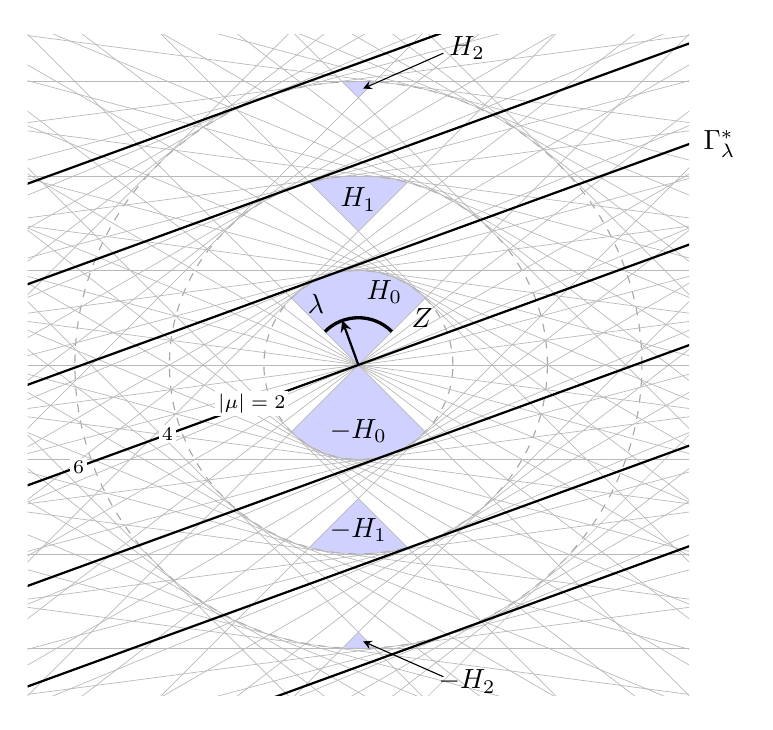
\begin{tikzpicture}[scale=0.6, >=stealth]
  \begin{scope}
    \clip (-7,-7) rectangle (7,7);
    \foreach \s in {1,-1}{
      \foreach \k in {0,1,2}{
        \begin{scope}[scale=\s, even odd rule]
          \clip (-13,-13) rectangle (13,13)
            (135:{2*\k+2}) arc (135:45:{2*\k+2}) -- (45:20) -- (135:20) -- cycle;
          \fill[blue!18] (0,{2*\k*sqrt(2)}) -- ({-sqrt(2)},{(2*\k+1)*sqrt(2)})
            -- (0,{(2*\k+2)*sqrt(2)}) -- ({sqrt(2)},{(2*\k+1)*sqrt(2)}) -- cycle;
        \end{scope}
      }
    }
    \foreach \r in {2,4,6}{ \draw[gray!70, dashed, thin] (0,0) circle (\r); }
    \foreach \t in {45,52.5,...,135}{
      \foreach \k in {-3,...,3}{
        \draw[gray!55, line width=0.25pt]
          ({2*\k*cos(\t)},{2*\k*sin(\t)}) +({\t+90}:14) -- +({\t-90}:14);
      }
    }
    \foreach \k in {-3,...,3}{
      \draw[black, line width=0.8pt]
        ({2*\k*cos(110)},{2*\k*sin(110)}) +(200:14) -- +(20:14);
    }
  \end{scope}
  \draw[very thick] (45:1) arc (45:135:1);
  \draw[->, thick] (0,0) -- (110:1);
  \node at (-0.9,1.3) {$\lambda$};
  \node at (1.35,1.0) {$Z$};
  \node at (0.55,1.55) {$H_0$};
  \node at (0,3.5) {$H_1$};
  \draw[->] (1.8,6.6) -- (0.1,5.85);
  \node at (2.3,6.7) {$H_2$};
  \node at (0,-1.4) {$-H_0$};
  \node at (0,-3.5) {$-H_1$};
  \draw[->] (1.8,-6.6) -- (0.1,-5.85);
  \node at (2.3,-6.7) {$-H_2$};
  \node[fill=white, inner sep=1pt] at (200:2.4) {\scriptsize $|\mu|=2$};
  \node[fill=white, inner sep=1pt] at (200:4.3) {\scriptsize $4$};
  \node[fill=white, inner sep=1pt] at (200:6.3) {\scriptsize $6$};
  \node[anchor=west] at (7.1,4.67) {$\Gamma^*_{\lambda}$};
\end{tikzpicture}
\caption{The visible frequencies for $m=2$ and $Z=\{\lambda\in S(\fz^*): 45^\circ\leq\arg\lambda\leq135^\circ\}$, so that $\delta=1-\cos45^\circ$ and $2/\delta\approx6.8$. The thin lines are $\mu\cdot\lambda=2k$ for $\lambda\in Z$ and $|k|\leq3$, and the $k$-th family envelops the dashed circle $|\mu|=2|k|$. The bold lines are $\Gamma_{\lambda}^*$ for one $\lambda\in Z$. The shaded regions are the holes $\pm H_k$, $0\leq k\leq2$, whose union is the complement of $\bigcup_{\lambda\in Z}\Gamma_\lambda^*$. $H_k=\emptyset$ for $k\geq3$, and every hole lies in $|\mu|<6<2/\delta$.}
\label{fig:visible}
\end{figure}
\begin{remark}
	By Proposition \ref{homogeneity}, if the conclusion of Theorem \ref{PW2} holds for $Z$ with constant $c$, then it holds for $tZ=\{t\lambda: \lambda\in Z\}$ with constant $ct^2$, for every $t>0$. In particular part 1 covers every band $\{|\lambda|\in [t, t(1+\eps)]\}$.
\end{remark}
As $\lambda$ ranges over a band or a cap, the hyperplanes $\Gamma_\lambda^*$ sweep out every frequency $|\mu|\geq c$. Only helices of large radius, $|\lambda|\to0$, resolve the low central frequencies, which is condition (i) of Corollary \ref{c:injSets}.


For functions with compact central support the band $|\mu|\leq c$ is recovered by analytic continuation.
\begin{corollary}\label{c:centralSupport}
	Let $f\in L^1(G)$ be supported in $\exp(\fv\times K)$ for some compact $K\subset \fz$. If $Z$ is a zero set of $If$, with $Z$ as in Theorem \ref{PW2}, then $f=0$. In particular, an arbitrarily small spherical cap of charges is an injectivity set for functions with compact central support.
\end{corollary}

\begin{proof}
	By Theorem \ref{PW2} and \eqref{e:Weyl}, $W_\mu(f^\mu)=0$ for $|\mu|>c$, so $f^\mu=0$ for $|\mu|>c$ by the injectivity of $W_\mu$ on $L^1(\fv)$ (Section \ref{s:Weyl}). For $\phi\in C_c(\fv)$, the function $\mu\mapsto \int_\fv f^\mu(x)\phi(x)dx$ is the Fourier transform of $u\mapsto \int_\fv f(x, u)\phi(x)dx\in L^1(\fz)$, supported in $K$, and so extends to an entire function on $\C^m$. It vanishes on the open set $\{|\mu|>c\}$, hence identically, and $f=0$.
\end{proof}

In Euclidean limited-angle tomography the data determine a function only microlocally, at the covectors conormal to some measured line, the \textit{visible} singularities of Quinto \cite{quintoSingularitiesXrayTransform1993}. The visible set is a cone in $T^*\R^n$, and the invisible part is recovered, if at all, by analytic continuation. On an $H$-type group the natural frequency space is not $T^*G$ but the unitary dual $\widehat G$, parameterized up to a Plancherel-null set by the central frequency \cite{bahouriFrequencySpaceHeisenberg2019, fischerQuantizationNilpotentLie2016}, and Corollary \ref{chargeFrequency} and Theorem \ref{PW2} are visible-frequency theorems in this sense. A band of charges, or a spherical cap when $\dim\fz\geq2$, determines the Fourier transform of $f$ at all central frequencies above a threshold. The visible set is a neighborhood of infinity in $\widehat G$ rather than a cone, the determination there is stable at each central frequency (Theorem \ref{t:stability}), and the invisible part, a bounded set of central frequencies, is recovered only by analytic continuation, for $f$ compactly supported in the central variable (Corollary \ref{c:centralSupport}).


\section{Sub-Riemannian Geometry of $H$-type groups}\label{sRGeometry}
\subsection{Hamiltonian Formalism}\label{HamFormalism}
We define the sub-Riemannian metric on $G$ by declaring $X_1, \ldots X_{2n}$ orthonormal, and the length of  $U_1, \ldots U_m$ to be infinite. This amounts to restricting the inner product $\langle , \rangle$ discussed in Section \ref{H-type} from all of   $\fg=\fv\oplus \fz$  to the first stratum $\fv$. Then any finite length smooth path in $G$ must be tangent to the nonintegrable distribution $\cD_q=TL_g(\fv)$. We call such a path \textit{horizontal}. The length of a horizontal path equals the length of its projection to the plane by the map
\begin{align*}
	dx: (x, u)\mapsto x\in \R^{2n}.
\end{align*}
A minimizing $H$-type geodesic is the shortest horizontal path joining two points of $G$. That any two points in $G$ are connected by a horizontal path is guaranteed by Chow's Theorem and the fact that $\cD$ satisfies the H\"{o}rmander condition (i.e. $\cD$ is bracket generating.)


 
The fiber-quadratic Hamiltonian $H: T^*G\to \R$ given in canonical coordinates by $$H=\tfrac{1}{2}\left(P_{X_{1}}^2+\cdots+P_{X_{2n}}^2\right)=\tfrac{1}{2}|\xi+\tfrac{1}{2}J_\mu x|^2$$
generates the geodesics. That is, any solution for Hamilton's equations for $H$ projects, via the canonical projection $T^*G\to G$, to a sub-Riemannian geodesic, and conversely, all geodesics arise in this way. To obtain geodesics parameterized by arclength, we only take solutions for which $H=1/2$. (Thus, we define the unit cotangent bundle $U^*G$ as the set of all $(q, p)\in T^*G$ for which $H(q, p)=1/2$).  

Geodesics are best understood by their projection to $\R^{2n}$: they are ``generalized helices." 
Indeed 
\begin{align*}
	\dot{p}_u=-\frac{\partial H}{\partial u}=0
\end{align*}
so that $\lambda=p_u$ is a constant of motion. 
 If we choose a basis for $\fv$ as in \eqref{symplecticBasis} that puts $J_\lambda$ into block diagonal form then $\fv$ is a direct sum of two-planes each invariant under $J_\lambda$. The geodesics projected to any one of these two-planes are either all  circles or lines.  
 If we interpret $\lambda$ as the ``generalized charge" of a particle, then Hamilton's equations for $H$, viewed as a Hamiltonian on $T^*\R^{2n}$, are just the Lorentz equations for a particle of charge $\lambda$ in a constant magnetic field. 

\subsection{Geodesic Flow}

The  Hamiltonian flow written in the coordinate $(x, u, \nu, \lambda)$ is exactly the left trivialization $T^*G\cong G\times \fg^*$. That is
\begin{align*}
	\varphi_s: G\times \fg^*\to G\times \fg^*
\end{align*}
The unique solution to Hamilton's equations for a curve starting at the origin with initial momentum $(\nu, \lambda)\in \fv^*\oplus\fz^*$  is
\begin{align*}
	s\mapsto \left(x(s), u(s), e^{sJ_\lambda}\nu, \lambda\right)\in G\times \fg^*
\end{align*}
with $x(s)$ and $u(s)$ given by
\begin{align}\label{geodesics}
	x(s)=
	\begin{cases}
		\frac{e^{sJ_\lambda}-1}{J_\lambda}{\nu}, & \lambda\neq 0\\
		s{\nu}, & \lambda=0
	\end{cases}, \qquad \qquad
	u(s)=
	\begin{cases}
		\left(\frac{|\lambda|s-\sin{(|\lambda|s)}}{2|\lambda|^2}\right)\frac{\lambda}{|\lambda|}|{\nu}|^2, & \lambda\neq 0 \\
		0, & \lambda=0
	\end{cases}.
\end{align}


The unique constant speed geodesic starting at the origin with initial momentum $(\nu, \lambda)\in \fv^*\oplus\fg^*$ is the projection to the $(x, u)$ component
\begin{align}
	s\mapsto (x(s), u(s)) \in G.\label{geodesic}
\end{align}

Motivated by Appendix \ref{momentumFunctions}, we view the geodesic flow in \textit{guiding center coordinates}: for $\nu\in S(\fv^*)$ and $\lambda\neq0$, left translation by $(J_\lambda^{-1}\nu, 0)$ moves the guiding center of \eqref{geodesic} to the origin and yields the curve
\begin{align*}
	\gamma_{\nu, \lambda}(s)=\left(J_\lambda^{-1}\nu, 0\right)(x(s), u(s))
\end{align*}
of \eqref{param}.
Moreover since $H$ and $\lambda$ are integrals of motion, the flow restricts to the $(H, \lambda)$-level sets
\begin{align*}
	\varphi_{s}: G\times S(\fv^*)\times\{\lambda\}\to G\times S(\fv^*)\times\{\lambda\}.
\end{align*}
The map
\begin{align*}
	\Phi: G\times S(\fv^*)\times(\fz^*\mz)\to\cG\setminus\cG_0, \qquad (x, u, \nu, \lambda)\longmapsto(x, u)\gamma_{\nu, \lambda},
\end{align*}
is onto. It is not injective: reparameterizing by $s\mapsto s+s_0$ in \eqref{param} gives
\begin{align}\label{e:reparam}
	\gamma_{\nu, \lambda}(s+s_0)=\big(0, \tfrac{s_0}{2}R\hat\lambda\big)\,\gamma_{e^{s_0J_\lambda}\nu, \lambda}(s),
\end{align}
so that $\Phi(x, u, \nu, \lambda)=\Phi\big((x, u)(0, \tfrac{s_0}{2}R\hat\lambda), e^{s_0J_\lambda}\nu, \lambda\big)$ for every $s_0\in \R$, and these are the only coincidences (Lemma \ref{l:fibers}). The fibers of $\Phi$ are lines, and $\dim\cG=2\dim G-2$, as for the space of lines in a Euclidean space of the same dimension.
\subsection{The Space of Geodesics}\label{spaceGeodesics}
Let $\cG_{\nu, 0}$ be the subset of geodesics of the form $(x, u)\gamma_{\nu, 0}$, with $\gamma_{\nu, 0}(s)=(s\nu, 0)$, and for $\nu\in S(\fv^*)$ set $I_{\nu, 0}f(x, u):=\int_\R f((x, u)\gamma_{\nu, 0}(s))\,ds$, which is well defined on $G/\R\nu$. Since left translation by an element of $G$ does not change the direction $\nu$, or the charge $\lambda=0$, the group $G$ acts on $\cG_{\nu, 0}$. Thus we may  parameterize that part of $\cG$ with $\lambda=0$ by 
\begin{align*}
	G\times S\fv^*\to \cG_{0}; \quad (x, u, \nu)\mapsto (x, u)\gamma_{\nu, 0}
\end{align*}
for $(x, u)\in G$ and $\nu\in S\fv^*$.

Since the action of $G$ on $\cG_{\nu, 0}$ is transitive, we obtain, for any fixed $\nu\in S\fv^*$, a parameterization of $\cG_{\nu, 0}$ by $G$ unique up to the isotropy subgroup $\R \nu:=\{r\nu: r\in \R\}$ fixing $\gamma_{\nu, 0}$. Therefore
\begin{align}\label{degGeo}
	\cG_{\nu, 0}\cong &G/\R\nu\cong T_\nu S^{2n-1}\times\fz\\
	\nonumber (x, u)\gamma_{\nu, 0}\mapsto &(x, u)\R\nu \mapsto ({{\rm Pr}}_\nu^\perp x, u)
\end{align}
where ${{\rm Pr}}_\nu^\perp(x)=x-\langle x, \nu\rangle \nu$ is the orthogonal projection. 
What's more, if $\cG_0$ is the subset of all geodesics with momentum $\lambda=0$, we have the identification
\begin{align*}
	\cG_0\to TS^{2n-1}\times \R^m. 
\end{align*}
For any $\nu\in S(\fv^*)$, let $d\nu^\perp du$ be the measure on $T_\nu S(\fv^*)\times\fz=\{(\eta, u)\in \fv^*\times\fz: \nu\cdot\eta=0\}$. Equip $\cG_{\nu, 0}$ with the same measure through the identification \eqref{degGeo}.


For $\lambda\neq0$, the orbit--stabilizer identification \eqref{e:orbitStabMain} of $\cG_{\nu, \lambda}$ with $G_\lambda=G/\Gamma_\lambda$ rests on the following description of the fibers of $\Phi$.
\begin{lemma}[Fibers of the parameterization]\label{l:fibers}
	Let $\lambda, \lambda'\in \fz^*\mz$, $\nu, \nu'\in S(\fv^*)$ and $(x, u), (x', u')\in G$. Then $(x, u)\gamma_{\nu, \lambda}$ and $(x', u')\gamma_{\nu', \lambda'}$ are the same oriented unparameterized geodesic if and only if $\lambda=\lambda'$ and there is $s_0\in \R$ with $\nu'=e^{s_0J_\lambda}\nu$ and $(x', u')=(x, u)(0, \tfrac{s_0}{2}|\lambda|^{-1}\hat\lambda)$. In particular the stabilizer of $\gamma_{\nu, \lambda}$ in $G$ is $\Gamma_\lambda$.
\end{lemma}
\begin{proof}
	Sufficiency is \eqref{e:reparam}. Conversely, two parameterizations by arclength of the same oriented geodesic differ by a shift, so $(x', u')\gamma_{\nu', \lambda'}(s)=(x, u)\gamma_{\nu, \lambda}(s+s_0)$ for all $s$ and some $s_0$. The charge is the central momentum, a constant of motion invariant under left translation, so $\lambda=\lambda'$. By \eqref{e:reparam} we may replace $(x, u)$ by $(x, u)(0, \tfrac{s_0}{2}|\lambda|^{-1}\hat\lambda)$ and $\nu$ by $e^{s_0J_\lambda}\nu$, and assume $s_0=0$. Comparing horizontal components in $(x', u')\gamma_{\nu', \lambda}(s)=(x, u)\gamma_{\nu, \lambda}(s)$ gives $x'+e^{sJ_\lambda}J_\lambda^{-1}\nu'=x+e^{sJ_\lambda}J_\lambda^{-1}\nu$ for all $s$, hence $x=x'$ and $\nu=\nu'$; then the central components give $u=u'$. For the stabilizer, take $(x, u)=(0, 0)$ and $\nu'=\nu$: then $e^{s_0J_\lambda}\nu=\nu$ forces $s_0\in 2\pi|\lambda|^{-1}\Z$, and $(x', u')=(0, j\pi|\lambda|^{-2}\hat\lambda)\in \Gamma_\lambda$.
\end{proof}
Let $d(x, u)$ be the Haar measure on $G$ determined by the orthonormal frame $X_1, \ldots, X_{2n}, U_1, \ldots U_m$. Also denote by $d(x, u)$ the Haar measure on $G/\Gamma_\lambda$ normalized so that 
\begin{align}\label{Haar2}
	\int_Gf(x, u)d(x, u)=\int_{G/\Gamma_\lambda}\sum_{(0, u')\in \Gamma_\lambda}f(x, u+u')d(x, u), \quad f\in C_c(G).
\end{align}
Equip $\cG_{\nu, \lambda}$ with the measure $d\cG_{\nu, \lambda}(x, u)=d(x, u)$ through its identification with $G/\Gamma_\lambda$. The orbits $\cG_{\nu, \lambda}$ partition $\cG_\lambda$ and depend on $\nu$ only through its orbit under $\{e^{sJ_\lambda}: s\in \R\}$ (Lemma \ref{l:fibers}), so $\cG_\lambda=\bigsqcup_{[\nu]\in \CP(\lambda, \fv^*)}\cG_{\nu, \lambda}$, where $\CP(\lambda, \fv^*):=S(\fv^*)/\{e^{sJ_\lambda}: s\in \R\}$. We give $\CP(\lambda, \fv^*)$ the measure $d\nu$ induced from the normalized surface measure on $S(\fv^*)$, and $\cG_\lambda$ the measure $d\cG_\lambda:=d\nu\, d\cG_{\nu, \lambda}$. This is well defined, since changing the representative $\nu$ changes the identification \eqref{e:orbitStabMain} by a translation, which preserves Haar measure. 


\section{Basic Properties of the X-ray Transform}\label{s:properties}
\subsection{Homogeneity}

For $\eps>0$ the dilation map $\delta_\eps(x, u)=(\eps x, \eps^2 u)$ is an isomorphism of the group $G$. Furthermore, 
\begin{align*}
	\delta_\eps: \Gamma_{\eps\lambda}\ni (0, k\pi|\eps\lambda|^{-2}\hat{\lambda})\longmapsto (0, k\pi |\lambda|^{-2}\hat{\lambda})\in \Gamma_{\lambda}, 
\end{align*}
so $\delta_\eps: G_{\eps\lambda}\to G_{\lambda}$ is well-defined. Denote by $\delta_\eps^*$ the pullback operator on functions
\begin{align*}
	&\delta_\eps^*: L^1(G)\to L^1(G), & \delta_\eps^*f=f\circ \delta_\eps\\
	&\delta_\eps^*: L^1(G_{\lambda})\to L^1(G_{\eps\lambda}), & \delta_\eps^*g=g\circ\delta_\eps.
\end{align*}
\begin{proposition}[Homogeneity]\label{homogeneity} For $f\in L^1(G)$, $\nu\in S(\fv^*)$ and $\lambda\in \fz^*\setminus\{0\}$
	\begin{align*}
		I_{\nu, \eps\lambda}(\delta_\eps^* f)(x, u)=(1/\eps)\,\delta_\eps^*\left(I_{\nu, \lambda}f\right)(x, u), \quad \forall \eps>0.
	\end{align*}
\end{proposition}
\begin{proof}
	The main observation is that
\begin{align*}
	\delta_\eps \gamma_{\nu, \eps\lambda}(s)=\gamma_{\nu, \lambda}(\eps s)
\end{align*}
Thus,
\begin{align*}
	I_{\nu, \eps\lambda}(\delta_\eps^* f)(x, u)
	&=\int_\R \delta_\eps^*f((x, u)\gamma_{\nu, \eps\lambda}(s))ds\\
	&=\int_\R f(\delta_\eps(x, u)\delta_\eps\gamma_{\nu, \eps\lambda}(s))ds\\
	&=\int_\R f(\delta_\eps (x, u)\gamma_{\nu, \lambda}(\eps s))ds\\
	&=(1/\eps)\int_\R f(\delta_\eps(x, u)\gamma_{\nu ,\lambda}(s))ds\\
	&=(1/\eps)(I_{\nu, \lambda} f)(\delta_\eps(x, u))
\end{align*}
as desired.
\end{proof}
\subsection{Boundedness and Factorization}
\begin{proposition}
	For any $\nu\in S(\fv^*)$, the X-ray transform $I_{\nu, 0}: L^1(G)\to L^1(G/\R\nu)$ is well-defined and bounded. 
\end{proposition}
\begin{proof}
	For $f\in C_c(G)$, 
	\begin{align*}
		\|I_{\nu, 0}f\|_{L^1(G/\R\nu)}
		&\leq\int_{\R^m} \int_{x\perp \nu}|I_{\nu, 0}f(x, u)|d\nu^\perp(x) du\\
		&\leq\int_{\R^m} \int_{x\perp \nu}\int_\R |f((x, u)(s\nu, 0))|dsd\nu^\perp(x)du\\
		&=\int_{\R^m}\int_{x\perp \nu} \int_\R| f(x+s\nu, u+s [x, \nu]/2)|dsd\nu^\perp(x)du\\
		&=\int_{\R^m}\int_{x\perp \nu} \int_\R| f(x+s\nu, u)|dsd\nu^\perp(x)du\\
		&=\int_{\fz}\int_{\fv}|f(x, u)|dxdu=\|f\|_{L^1(G)}.
	\end{align*}
Therefore, $I_{\nu, 0}$ extends to a bounded map between $L^1$ spaces.
\end{proof}
Here we decompose the X-ray transform into a periodization map and a special case of the Pompeiu Transform. (See \cite{agranovskyInjectivityPompeiuTransform1994}).
\begin{proposition}\label{factorization}
	For any $\lambda\in \mathfrak{z}^*\setminus \{0\}$ and $\nu\in S(\fv^*)$, the X-ray transform $I_{\nu, \lambda}: L^1(G)\to L^1(G_\lambda)$ is well-defined, bounded and factors in the following way:
	\[ 
	\begin{tikzcd}
		L^1(G) \arrow[d, "P_{\lambda}" left=1]  \arrow[r, "{I}_{\nu, \lambda}"]  &L^1(G_\lambda)\\
		L^1(G_{\lambda}) \arrow[ur, "\widetilde{I}_{\nu, \lambda}" below=10, pos=0.75]
	\end{tikzcd}
	\]
	where the maps which we call \textit{central periodization} and the \textit{holonomy transform} are given by 
	\begin{align*}
		P_{\lambda}f(x, u)=\sum_{k\in\mathbb{Z}}f(x, u+\pi k |\lambda|^{-2}\hat{\lambda}), 
		\quad \quad
		\widetilde{I}_{\nu, \lambda}g(x, u)=\int_0^{2\pi |\lambda|^{-1}}g\left( (x, u)\gamma_{\nu, \lambda}(s)\right)ds
	\end{align*}
	for $f\in L^1(G)$ and $g\in L^1(G_\lambda)$.
\end{proposition}
\begin{proof}
	By the dominated convergence theorem we have
	\begin{align*}
		\int_{G_{\lambda}}P_{\lambda}f(x, u)d(x, u)=\int_G f(x, u)d(x, u), \quad f\in C_c^\infty(G).
	\end{align*}
	In particular $$\|P_{\lambda}f\|_{L^1(G_{\lambda})}\leq \|f\|_{L^1(G)}.$$
	
	Now $\widetilde{I}_{\nu, \lambda}f$ is just a group convolution operator on $G_{\lambda}$ by a compactly supported convolution kernel. Hence it is bounded. In particular, 
	\begin{align*}
		|\widetilde{I}_{\nu, \lambda}f(x, u)|\leq \int_0^{2\pi |\lambda|^{-1}}|f\left((x, u)\gamma_{\nu, \lambda}(s)\right)|ds
	\end{align*}
	and 
	\begin{align*}
		\int_{G_\lambda}|\widetilde{I}_{\nu, \lambda} f(x, u)|d(x, u)
		&=\int_0^{2\pi |\lambda|^{-1}} \int_{G_\lambda}|f\left(x, u\right)|d(x, u)ds.
	\end{align*}
	Therefore
	\begin{align*}
		\|\widetilde{I}_{\nu, \lambda} f\|_{L^1(G_\lambda)}\leq 2\pi  |\lambda|^{-1}\|f\|_{L^1(G_{\lambda})}.
	\end{align*}
	The decomposition follows from the helical symmetry \eqref{e:helicalSym} of the geodesics. For $f\in C_c^\infty(G)$ 
	\begin{align*}
		\widetilde{I}_{\nu, \lambda}\circ P_{\lambda}f(x, u)
		&=\int_0^{2\pi  |\lambda|^{-1}}\sum_{k\in\mathbb{Z}}f\left((x, u+\pi k|\lambda|^{-2}\hat{\lambda})\gamma_{\nu, \lambda}(s)\right)ds\\
		&=\int_0^{2\pi  |\lambda|^{-1}}\sum_{k\in\mathbb{Z}}f\left((x, u)\gamma_{\nu, \lambda}(s+2\pi k|\lambda|^{-1})\right)ds	\\
		&=\sum_{k\in\mathbb{Z}}\int_{2\pi k |\lambda|^{-1}}^{2\pi (k+1) |\lambda|^{-1}}f\left((x, u)\gamma_{\nu, \lambda}(s)\right)ds	\\
		&=\int_\R f\left((x, u)\gamma_{\nu, \lambda}(s)\right)ds=I_{\nu, \lambda}f(x, u)
	\end{align*}
	where the second to last equality follows from the dominated convergence theorem. 
	
	By the previous two statements, we have
	\begin{align*}
		\| I_{\nu, \lambda} f\|_{L^1(G_\lambda)}\leq 2\pi |\lambda|^{-1}\|f\|_{L^1(G)}.
	\end{align*}
	In particular $I_{\nu, \lambda}$ extends to a bounded map from $L^1(G)$ to $L^1(G_\lambda)$. 
\end{proof}

\begin{proposition}
		Let $\chi\in M(\fz^*)$ be any positive compactly supported Radon measure for which
		\begin{align}\label{centralWeight}
			\int_{\fz^*}|\lambda|^{-1}d\chi(\lambda)<\infty,
		\end{align}
	and let $\chi d\cG$ be the measure on the space of geodesics defined by
	\begin{align*}
		\int_{\cG}F \chi d\cG=\int_{\lambda\in \fz^*}\int_{\cG_\lambda}F d\cG_\lambda d\chi(\lambda), \quad F\in C_c^\infty(\cG).
	\end{align*}
		The full X-ray transform $I: L^1(G)\to L^1(\cG, \chi d\cG)$ is well-defined and bounded. 
\end{proposition}
\begin{proof}
	\begin{align*}
		\|If\|_{L^1(\cG, \chi d\cG)}
		&=\int_{\cG}|If| \chi d\cG\\
		&=\int_{\lambda\in \fz^*}\int_{\cG_\lambda}|If|\, d\cG_\lambda\, d\chi(\lambda)\\
		&=\int_{\lambda\in \fz^*}\int_{\CP(\lambda, \fv^*)}\int_{G_{\lambda}}|I_{\nu, \lambda}f(x, u)|\, d(x, u)\, d\nu\, d\chi(\lambda)\\
		&\leq2\pi \int_{\fz^*}|\lambda|^{-1}d\chi(\lambda)\,\|f\|_{L^1(G)}
	\end{align*}
	which proves boundedness in view of the assumption \eqref{centralWeight}. 
\end{proof}


\section{Representation Theory of $G$ and $G_\lambda$}\label{s:representations}
The Fourier transform on $G$ is defined by means of irreducible unitary representations. 
There are many choices of conventions for representations of the Heisenberg group. We choose to use the Bargmann-Fock representation because certain intertwining operators are more explicit than for the Schr\"{o}dinger representation.  %

\subsection{Bargmann-Fock  Representation on the Heisenberg group}\label{BF}
Bargmann-Fock space is the following Hilbert space (equipped with the evident inner product)
\begin{align*}
	\cF(\C^n):=\{F: \C^n\to \C, \text{ holomorphic: }\frac{1}{\pi^n}\int_{\C^n}|F(\zeta)|^2e^{-|\zeta|^2}<\infty\}.
\end{align*}
An orthonormal basis is given by
\begin{align*}
	\omega_\alpha=\zeta^\alpha/\sqrt{\alpha!}, \quad \zeta\in \C^n, \; \alpha\in \N^n 
\end{align*}
For each $h\in \R^*$ the Bargmann-Fock representation is the map
\begin{align*}
	{\pi}_h: \heis_n \to \cU(\cF(\C^n))
\end{align*}
given by 
\begin{align*}
	{\pi}_{h}(z, t)F(\zeta):=e^{i ht-\sqrt{h/2}\zeta\cdot\overline{z}-\tfrac{ h}{4}|z|^2}F(\zeta+\sqrt{h/2}z), \quad F\in \cF(\C^n), \quad h>0,
\end{align*}
and ${\pi}_h(z, t)={\pi}_{|h|}(\overline{z}, -t)$ for $h<0$. Despite the dependence on a parameter $h\in \R^*$, we simply refer to this as \textit{the} Bargmann-Fock representation. Here $\zeta\cdot \overline{z}=\zeta_1\overline{z}_1+\cdots + \zeta_n\overline{z}_n$. The Bargmann-Fock representation is a strongly continuous unitary irreducible representation of the Heisenberg group on $\cF(\C^n)$. 

\begin{remark}
	There are many other normalizations out there, but we have chosen the one for which
	\begin{itemize}
		\item ${\pi}_h(z, t)=e^{iht}{\pi}_h(z, 0)$
		\item ${\pi}_*(X_j-iY_j)=\sqrt{2h}\,\partial_{\zeta_j}$ and ${\pi}_*(X_j+iY_j)=-\sqrt{2h}\,\zeta_j$ for $h>0$, so that $\pi_*(-\Delta_{\rm{sr}})=h\sum_{j=1}^n(2\zeta_j\partial_{\zeta_j}+1)$ for the sub-Laplacian $\Delta_{\rm{sr}}=\sum_j X_j^2+Y_j^2$, with eigenvalue $h(2l+n)$ on the homogeneous polynomials of degree $l$.
	\end{itemize}
\end{remark}

\subsection{Bargmann-Fock  Representation on $H$-type groups}\label{BargmannFock}
To construct representations on a general $H$-type group, we follow  \cite{mullerSharpLpEstimates2008}. Given $\mu\in \mathfrak{z}^*\setminus\{0\}$ consider the operator $J_\mu:\mathfrak{v}\to\mathfrak{v}$. If $|\mu|=1$, then $J_\mu^2=-I$. In particular, $J_\mu$ has eigenvalues $\pm i$, and since it is orthogonal, there exists an orthonormal basis 
\begin{align}
	P_1^\mu, \ldots, P^\mu_n, Q_1^\mu, \ldots, Q_n^\mu\label{symplecticBasis}
\end{align}
of $\mathfrak{v}$ which is symplectic with respect to the form $\omega_\mu$. 

This means that, for every $\mu\in \mathfrak{z}^*\setminus \{0\}$, there exists an orthogonal transformation $R_\mu=R_{\mu/|\mu|}: \R^{2n}\to \mathfrak{v}$ such that
\begin{align}\label{normalForm}
	J_\mu=|\mu|R_\mu J R_\mu^t
\end{align}
where $J=\begin{bmatrix}
	0& -I \\
	I& 0
\end{bmatrix}$
with respect to the basis \eqref{symplecticBasis}.

\begin{remark}
    In general there is no continuous global assignment $\mu\mapsto R_\mu$  for all $\mu\in \fz^*\mz$. Indeed, the set of $J_\mu$ for $\mu\in \fz^*\mz$ forms a $S^{m-1}$ sphere over which the set of possible $R_\mu$ for $\mu\in \fz^*\mz$, forms  principle $U(n)$ bundle. One may still choose $R_\mu$ smoothly locally in  $\mu$.
\end{remark}
\begin{lemma}
	The mapping $\alpha_\mu: G\to \mathbb{H}_n$ defined by
	\begin{align*}
		\alpha_\mu(x, u)=(R_\mu^t x, \tfrac{\mu\cdot u}{|\mu|}), \quad (x, u)\in \mathbb{R}^{2n}\times\mathbb{R}^m
	\end{align*}
	is a homomorphism.
\end{lemma}

Then define the irreducible representations of $G$ on $\cF(\C^n)$ by 
\begin{align}\label{e:repH}
	\pi_\mu:={\pi}_{|\mu|}\circ\alpha_\mu. 
\end{align}
\begin{remark}
	When $\mu\in \fz^*\mz$ we assume it is clear that $\pi_\mu$ is a representation of an $H$-type group $G$ with center $\fz$; when $h=|\mu|$ is a scalar, $\pi_h$ is a representation of the Heisenberg group $\heis_n$. 
\end{remark}
Since $R_\mu$ is orthogonal, $d\alpha_\mu$ carries the sub-Laplacian $\Delta_{\rm{sr}}=\sum_{j=1}^{2n}X_j^2$ of $G$ to that of $\heis_n$, so by the remark in Section \ref{BF}, $d\pi_\mu(-\Delta_{\rm{sr}})=|\mu|\sum_{j=1}^n(2\zeta_j\partial_{\zeta_j}+1)$, with eigenvalue $|\mu|(2l+n)$ on the homogeneous polynomials of degree $l$.
\subsection{Intertwiners}
Let $S\in Sp(2n, \R)$ and $h>0$. Then $(z, t)\mapsto\pi_h(Sz, t)$ is an irreducible unitary representation of $\heis_n$ with the same central character as $\pi_h$, so by the Stone--von Neumann theorem there is a unitary operator $\tau(S)$ on $\cF(\C^n)$, unique up to a phase, such that
\begin{align}\label{e:intertwine}
    \pi_h(Sz, t)=\tau(S)\circ\pi_h(z, t)\circ\tau(S)^*, \quad (z, t)\in \heis_n.
\end{align}
The projective representation $S\mapsto\tau(S)$ is the metaplectic representation \cite[Ch.~4]{follandHarmonicAnalysisPhase1989}. We use $\tau(S)$ only through the conjugation, which does not depend on the phase. On the unitary group we fix a choice:
\begin{definition}\label{d:tau}
	For $U\in U(n)=Sp(2n, \R)\cap O(2n, \R)$, identified with the unitary group of $\C^n\cong(\R^{2n}, J)$, and $F\in \cF(\C^n)$, define
	\begin{align*}
		{\tau}(U)F(\zeta):=F(U^*\zeta), \quad \zeta \in \C^n.
	\end{align*}
\end{definition}
This is a unitary representation of $U(n)$ which preserves the homogeneous polynomials of each degree and satisfies \eqref{e:intertwine}:
\begin{lemma}\label{l:rotateAxis}
    Let $u\in \R^{2n}$ with $|u|=1$.  For any $U\in U(n)$ the operator $\tau(U)$  is unitary on $\cF(\C^n)$, preserves $\cE_l:={\rm Span}_\C\{\omega_\alpha: |\alpha|=l\}$ for every $l\in \N$, and satisfies
    \begin{align*}
        \pi_h(Uz, t)=\tau(U)\circ\pi_h(z, t)\circ\tau(U)^*, \quad (z, t)\in \heis_n, \; h>0.
    \end{align*}
\end{lemma}

\begin{proof}
    The group $U(n)$ acts transitively on the unit sphere of $\C^n$. The substitution $\zeta\mapsto U^*\zeta$ preserves the Gaussian measure $\pi^{-n}e^{-|\zeta|^2}$, so $\tau(U)$ is unitary, and it preserves the homogeneous polynomials of each degree. Since $(U^*\zeta)\cdot\overline{z}=\zeta\cdot\overline{Uz}$ and $|Uz|=|z|$,
    \begin{align*}
        \tau(U)\circ{\pi}_{h}(z, t)\circ\tau(U)^*F(\zeta)
        =e^{i ht-\sqrt{h/2}\,(U^*\zeta)\cdot\overline{z}-\tfrac{ h}{4}|z|^2}F(\zeta+\sqrt{h/2}\, Uz)
        ={\pi}_h(Uz, t)F(\zeta).\qedhere
    \end{align*}
\end{proof}

\subsection{Finite Dimensional Representations on $H$-type groups}
For any $\eta\in \fv^*$ define 
\begin{align}\label{finiteRep}
	\pi_{\eta, 0}(x, u)=e^{i\eta(X) }, \quad (x, u)=\exp(X+U)\in G, \quad \text{with } X\in \fv, \; \text{and }U\in \fz.
\end{align}
Then $\pi_{\eta, 0}: G\to U(1)$ is a one dimensional unitary representation of $G$ on $\C$. 


\subsection{The Unitary Dual}
The \textit{unitary dual} $\widehat{G}$ of a group $G$ is the set  of its irreducible unitary representations up to unitary equivalence. That is, the set of pairs $(\cH_\pi, \pi)$ where $\cH_\pi$ is a Hilbert space, and $\pi: G\to \cU(\cH_\pi)$ is a strongly continuous group homomorphism from $G$ to the set of unitary operators on $\cH_\pi$. When $G$ is a nilpotent Lie group,  Kirillov theory establishes a bijection between $\widehat{G}$ and orbits of $\fg^*$ by the coadjoint action. 

When $G$ is an $H$-type group, the Kirillov correspondence associates to each $\eta\in \fv^*$  the representation $\pi_{(\eta,  0)}$ in \eqref{finiteRep} acting on $\cH_{\pi_{\eta, 0}}=\mathbb{C}$, and to each $\mu\in \fz^*\mz$ the infinite dimensional representation $\pi_{\mu}$  acting on $\cH_{\pi_\mu}=\cF(\C^n)$. Since $\fv^*\cup \fz^*\mz$ exhausts all representatives of the coadjoint orbits of $\fg^*$, all elements of $\widehat{G}$ are obtained in this way \cite{kirillovUnitaryRepresentationsNilpotent1962}. Therefore $\widehat{G}$ is parameterized by $\fv^*\cup \fz^*\setminus\{0\}$:  
\begin{align*}
	\widehat{G}=\{\text{class of } \pi_{\eta, 0}: \eta\in \fv^*\}\cup \{\text{class of } \pi_\mu: \mu \in \fz^*\setminus\{0\}\}.
\end{align*}
\subsection{Representations on $G_\lambda$}

\begin{proposition}[Compatibility of momenta]\label{propCompatibility}
	For $\mu\in \fz^*\mz$ and the associated representation $\pi_\mu$ of $G$,  there exists a representation  of $G_\lambda$ also denoted by $\pi_\mu$ making the following diagram
	\[ 
	\begin{tikzcd}
		G \arrow[d]  \arrow[r, "\pi_\mu"]  & \cU(\cF(\C^n))\\
		G_{\lambda} \arrow[ur, "\pi_\mu" below=7, pos=0.5]
	\end{tikzcd}
	\]
	commute if and only if 
	\begin{align*}
		\mu\cdot \lambda=2|\lambda|^3k, \quad \text{ for some } k\in \Z. 
	\end{align*}
	That is, $\pi_\mu$ descends from an irreducible unitary representation of $G$ to one of  $G_\lambda$ if and only if $\mu$ is an element of the dual of the subgroup $\Gamma_\lambda$ excluding zero. 	
\end{proposition}
\begin{proof}
	Fix $\lambda\in \fz^*\mz$. Then $\pi_\mu$ is a representation of $G_\lambda$ if and only if $\Gamma_\lambda\subset \ker{\pi_\mu}$. Since $\pi_\mu(x, u)=e^{i\mu\cdot u}\pi_\mu(x, 0)$, we have 
	\begin{align*}
		\ker\pi_\mu 
		&=\{(x, u)\in G: \pi_\mu(x, u)={{\rm Id}}_{\cF(\C^n)}\}\\
		&=\{(0, u)\in G: u\cdot \mu\in 2\pi\Z \}.
	\end{align*}
	Then $\Gamma_\lambda=\{(0, l\pi|\lambda|^{-2}\, \hat{\lambda}): l\in \Z\}\subset \ker{\pi_\mu}$ if and only if
	\begin{align*}
		\pi |\lambda|^{-2}\,\hat{\lambda}\cdot \mu =2\pi k, \quad k\in \Z.
	\end{align*}
	This is precisely the condition that $\mu$ lies in the annihilator $\Gamma_\lambda^*:=\{\mu\in \fz^*: \mu\cdot\omega\in 2\pi \Z, \text{for all }\omega\in \Gamma_\lambda\}$ of the central lattice. We have
	
	

	\begin{align}
		\mu\cdot \lambda=2|\lambda|^3k, \quad k\in \mathbb{Z} \label{compadability}
	\end{align}
as desired. 
\end{proof}
\begin{remark}
	Equation \eqref{compadability} implies
		\begin{align*}
		\mu=\mu_\perp+2k|\lambda|\lambda
	\end{align*}
where $\mu_\perp\in \fz^*$ such that $\mu_\perp\cdot\lambda=0$. 
\end{remark}
\begin{remark}
	Note $k=0$ in Equation \eqref{compadability} if and only if $\lambda, \mu\in \fz^*\mz$ are perpendicular. This is only possible when $m=\dim \fz >1$. 
\end{remark}

By Proposition \ref{propCompatibility}, we may view the unitary dual $\widehat{G}_\lambda$ as a subset of $\widehat{G}$. 
\begin{align*}
	\widehat{G}_\lambda=\{\text{class of }\pi_{\eta, 0}: \eta\in \fv^*\}\cup \{\text{class of } \pi_\mu:  \mu\in \Gamma_\lambda^*\mz \}\subset \widehat{G}
\end{align*}
where
\begin{align*}
	\Gamma_\lambda^*:=\{\mu\in \fz^*:  \mu\cdot \lambda=2k|\lambda|^3, \, k\in \Z\}\subset \fz^*
\end{align*}
is the dual to the discrete subgroup $\Gamma_\lambda$. 

\begin{remark}\label{conjRmk}
	For any $\lambda\in \fz^*\mz$ the geodesic $\gamma_{\nu, \lambda}(s)$ starting at $s=0$ reaches its first conjugate point at $s=2\pi R$, $R=|\lambda|^{-1}$ (see \cite{montgomeryTourSubriemannianGeometries2006}), and the two points in conjugacy differ by a group translation of $(0, \pi R^2 \hat{\lambda})\in G$ with $\hat{\lambda}=|\lambda|^{-1}\lambda$. Indeed
	\begin{align*}
		\gamma_{\nu, \lambda}(s+2\pi R)=(0, \pi R^2\hat{\lambda})\gamma_{\nu, \lambda}(s)
	\end{align*}
	On the other hand, the representation $\pi_{\mu}$ which is a map from $G$ to unitary operators on Bargmann-Fock space $\cF(\C^n)$, while satisfying the left-invariance $\pi_{\mu}((x, u)\gamma_{\nu, \lambda}(s)) =\pi_{\mu}(x, u)\pi_{\mu}(\gamma_{\nu, \lambda}(s))$ also satisfies
	\begin{align*}
		\pi_\mu(0, \pi R^2\hat{\lambda})=\pi_{\mu}(0, 0)=I
	\end{align*}
	whenever $\mu\cdot\lambda=2k|\lambda|^3$, and therefore
	\begin{align*}
		\pi_\mu((x, u)\gamma_{\nu, \lambda}(s+2\pi R))=\pi_\mu((x, u)\gamma_{\nu, \lambda}(s)).
	\end{align*}
\end{remark}
\subsection{Schr\"{o}dinger  Representation on the Heisenberg group}
Denote by $\mathcal{U}(L^2(\mathbb{R}^n))$ the set of unitary operators acting on $L^2(\mathbb{R}^n)$. For each $h\in \mathbb{R}\setminus \{0\}$ the map
\begin{align*}
	\rho_h: \mathbb{H}_n\longrightarrow \mathcal{U}(L^2(\mathbb{R}^n))
\end{align*}
\begin{align*}
	[\rho_h(x, y, t)\phi](\xi)=e^{ih(t+\frac{1}{2}xy)}e^{i\sqrt{h}y\xi}\phi(\xi+\sqrt{|h|}x), \quad \phi\in L^2(\mathbb{R}^n)
\end{align*}
where $\sqrt{h}=\text{sgn}(h)\sqrt{|h|}$. Here we are more or less using the conventions of Strichartz \cite[p. 358]{strichartzLpHarmonicAnalysis1991} and \cite{fischerQuantizationNilpotentLie2016}.

This is a strongly continuous unitary representation of $\mathbb{H}_n$ on $L^2(\mathbb{R}^n)$.  These \textit{Schr\"{o}dinger representations} are irreducible and pairwise inequivalent. Moreover, by the Stone-von Neumann Theorem, they exhaust all of the irreducible unitary representations, up to unitary equivalence, that are nontrivial on the center of $\mathbb{H}_n$.

\begin{remark}
	There are many other realizations of the Schr\"{o}dinger representation, but we have chosen the one for which
	\begin{itemize}
		\item $\rho_h(z, t)=e^{iht}\rho_h(z, 0)$
		\item $\rho_*X=\partial_\xi$
		\item $\rho_*Y=i\xi$. 
	\end{itemize}
\end{remark}
The Bargmann-Fock Representation ${\pi}_h$ is unitarily equivalent to the Schr\"{o}dinger representation $\rho_{ h}$ with the intertwining map $B: L^2(\R^n)\to \cF(\C^n)$ given by
\begin{align}\label{Bargmann}
	Bf(\zeta)=\pi^{-n/4}e^{-\frac{1}{2}\zeta\cdot\zeta}\int_{\R^n}f(\xi)e^{\sqrt{2}\xi\cdot\zeta -\frac{1}{2}|\xi|^2}d\xi
\end{align}
That is, $\pi_h(z, t)\circ B=B\circ\rho_h(z, t).$ This can be seen by taking the generating series for the Hermite functions:
\begin{align*}
	\pi^{-n/4}e^{\sqrt{2}\xi\cdot\zeta-\zeta\cdot\zeta/2-|\xi|^2/2}=\sum_{\alpha\in \N^n}\Phi_\alpha(\xi)\omega_\alpha(\zeta).
\end{align*}
\subsection{Schr\"{o}dinger  Representation on $H$-type groups}
Returning to $H$-type groups, let $\mu\in \fz^*\setminus\{0\}$. 
The map
\begin{align*}
	\rho_\mu:=\rho_{|\mu|}{\circ}\,\alpha_\mu
\end{align*}
is an irreducible unitary representation of $G$ acting on $L^2(\mathbb{R}^n)$. In fact, any irreducible representation of $G$ with central character $e^{i\mu\cdot u}$ is unitarily equivalent to $\pi_\mu$. All irreducible unitary representations that are nontrivial on the center of $G$ are unitarily equivalent to one such $\pi_\mu$.
\begin{remark}
	We assume it is understood that when $\mu\in \fz^*\mz$, the map $\rho_\mu$ is the Schr\"{o}dinger representation on the $H$-type group $G$; when $h=|\mu|$ is a scalar, $\rho_h$ is a representation of the Heisenberg group $\heis_n$. 
\end{remark}


\subsection{The Weyl transform}\label{s:Weyl}
For $\mu\in \fz^*\mz$ and $\phi\in L^1(\fv)$ define
\begin{align}\label{e:WeylDef}
	W_\mu(\phi):=\int_\fv\phi(x)\pi_\mu(x, 0)^*dx.
\end{align}
By \eqref{e:repH}, $W_\mu(\phi)=\int_{\R^{2n}}(\phi\circ R_\mu)(z)\,\pi_{|\mu|}(z, 0)^*dz$ is the Weyl transform on $\heis_n$ at the parameter $|\mu|$ \cite{thangaveluHarmonicAnalysisHeisenberg1998, follandHarmonicAnalysisPhase1989} of $\phi\circ R_\mu$. Since $R_\mu$ is orthogonal, $\phi$ and $\phi\circ R_\mu$ have the same $L^p$ norms, so properties of the Weyl transform on $\heis_n$ transfer to $W_\mu$ verbatim: $W_\mu$ is injective on $L^1(\fv)$ \cite{thangaveluHarmonicAnalysisHeisenberg1998}. When $m=1$ and $\mu>0$ one may take $R_\mu={\rm id}$, and $W_\mu$ is the classical Weyl transform at the parameter $\mu$.

\begin{proposition}[Plancherel identity for the Weyl transform]\label{p:PlancherelWeyl}
	Let $\mu\in \fz^*\mz$ and $\phi\in L^1\cap L^2(\fv)$. Then $W_\mu(\phi)$ is Hilbert--Schmidt and
	\begin{align}\label{e:PlancherelWeyl}
		\|W_\mu(\phi)\|^2_{HS}=(2\pi)^n|\mu|^{-n}\|\phi\|^2_{L^2(\fv)}.
	\end{align}
\end{proposition}
\begin{proof}
	Write $h=|\mu|$ and $\phi_\mu:=\phi\circ R_\mu$. By \eqref{e:repH} and the unitary equivalence $B$ of \eqref{Bargmann} between $\pi_{|\mu|}$ and $\rho_{|\mu|}$, the operator $W_\mu(\phi)$ has the same Hilbert--Schmidt norm as $W_h(\phi_\mu):=\int_{\R^{2n}}\phi_\mu(z)\rho_h(z, 0)^*dz$. From the definition of $\rho_h$, $W_h(\phi_\mu)$ has integral kernel
	\begin{align*}
		K(\xi, \xi')=h^{-n/2}\int_{\R^n}\phi_\mu\Big(\frac{\xi-\xi'}{\sqrt h}, y\Big)e^{-i\sqrt h\, y\cdot\frac{\xi+\xi'}{2}}dy,
	\end{align*}
	and the change of variables $(\xi, \xi')\mapsto\big(\frac{\xi-\xi'}{\sqrt h}, \sqrt h\frac{\xi+\xi'}{2}\big)$ has unit Jacobian, so by the Euclidean Plancherel theorem in $y$,
	\begin{align*}
		\|W_h(\phi_\mu)\|_{HS}^2=h^{-n}\int_{\R^{2n}}\Big|\int_{\R^n}\phi_\mu(a, y)e^{-iy\cdot b}dy\Big|^2da\, db=(2\pi)^nh^{-n}\|\phi_\mu\|^2_{L^2(\R^{2n})}.
	\end{align*}
	Since $R_\mu$ is orthogonal, $\|\phi_\mu\|_{L^2(\R^{2n})}=\|\phi\|_{L^2(\fv)}$, which is \eqref{e:PlancherelWeyl}.
\end{proof}

\section{Group Fourier Analysis}\label{GFT}
Motivated by the Peter--Weyl Theorem for compact Lie groups, we consider the unitary dual as a generalized frequency space for the group Fourier transform. See \cite{fischerQuantizationNilpotentLie2016} for a detailed exposition on the topic, and \cite{follandHarmonicAnalysisPhase1989, gellerFourierAnalysisHeisenberg1977, thangaveluHarmonicAnalysisHeisenberg1998} for the harmonic analysis of the Heisenberg group. 
For any $\pi\in \widehat{G}$, we define the group Fourier transform of an integrable function $f\in L^1(G)$ to be the operator $\cF(f)(\pi)\in \mathcal{L}(\cH_\pi)$ defined by
\begin{align*}
	\mathcal{F}(f)(\pi)=\int_Gf(g)\pi(g)^*dg.
\end{align*}
For $\mu\in \fz^*\mz$ or $\eta\in \fv^*$, we write $\cF(f)(\mu)=\cF(f)(\pi_\mu)$ and $\cF(f)(\eta, 0)=\cF(f)(\pi_{(\eta, 0)})$. For $f\in L^1(G)$, its Fourier transform $\pi\mapsto \cF(f)(\pi)$ is a bounded family of bounded operators on $\cH_\pi$, indexed by $\widehat{G}=\fv^*\cup \fz^*\mz$. The Fourier transform extends to an isometry from $L^2(G)$ onto the Hilbert space $L^2(\widehat{G})$ of all measurable  families $\{A(\mu)\}_{\mu\in \fz^*\mz}$ of operators on $\cH_{\pi_\mu}$ which are Hilbert-Schmidt for almost every $\mu\in \fz^*\mz$, with norm
\begin{align*}
	\|A\|:=\left(\int_{\fz^*\mz}\|A(\mu)\|^2_{HS(\cH_\mu)}d\pi(\mu)\right)^{\frac{1}{2}}<\infty
\end{align*}
where $d\pi(\mu)=c_0|\mu|^nd\mu$, for a constant $c_0>0$ depending on $n$ and $m$, is the \textit{Plancherel measure}.
This is the unique measure on $\widehat{G}$ for which the Plancherel formula holds:
\begin{align*}
	\int_G |f(g)|^2dg=c_0\int_{\fz^*\mz}\|\cF(f)(\mu)\|^2_{HS(\cH_\mu)}|\mu|^nd\mu.
\end{align*}
Note that only the $\fz^*\mz$ part of the unitary dual appears in the Plancherel formula. This is because the subset of $\widehat{G}$  corresponding to $\fv^*$ of finite dimensional representations has measure zero. 
The Plancherel Formula yields an inversion formula for $f\in \mathcal{S}(G)$: 
\begin{align*}
	f(g)=\int_{\widehat{G}}{\rm tr}\left(\pi(g)\mathcal{F}(f)(\pi)\right)d\pi.
\end{align*}
\subsection{Fourier Transform on $G_\lambda$}
Fix $\lambda\in \fz^*\mz$. For $f\in C_c^\infty(G_\lambda)$ and $\mu\in \fz^*\setminus\{0\}$ satisfying \eqref{compadability} let 
\begin{align*}
	\mathcal{F}_\lambda(f)(\pi_\mu)=\int_{G_\lambda}f(g)\pi_\mu^*(g)dg
\end{align*}
Note that the Fourier transform $\cF_\lambda(f)(\pi_\mu)$ on $G_\lambda$ is only defined for $\mu\in \Gamma_\lambda^*$. 

For $\eta\in \fv^*$ we have
\begin{align*}
	\cF_\lambda(f)(\pi_{(\eta, 0)})=\int_{\fv}f_0(x)e^{-i\langle \eta, x\rangle}dx
\end{align*}
where $f_0(x)=\int_{\fz/\Gamma_\lambda}f(x, u)du$.

\begin{theorem}[Plancherel theorem on $G_\lambda$]\label{t:PlancherelQuotient}
	Let $F\in L^1(G_\lambda)\cap L^2(G_\lambda)$ and, for $\mu\in \Gamma_\lambda^*$, let $F^\mu(x)=\int_{\fz/\Gamma_\lambda}F(x, u)e^{-i\mu\cdot u}du$ as in \eqref{e:centralFT}. Write $\mu=\mu_\perp+2k|\lambda|^2\hat\lambda$ with $\mu_\perp\in \lambda^\perp$ and $k\in \Z$. Then
	\begin{align}\label{e:PlancherelCentral}
		\int_{G_\lambda}|F(x, u)|^2d(x, u)=\frac{|\lambda|^2}{\pi(2\pi)^{m-1}}\sum_{k\in \Z}\int_{\lambda^\perp}\big\|F^{\mu_\perp+2k|\lambda|^2\hat\lambda}\big\|^2_{L^2(\fv)}d\mu_\perp,
	\end{align}
	where for $m=1$ the integral over $\lambda^\perp=\{0\}$ is evaluation at $\mu_\perp=0$. Moreover, for almost every $\mu\in \Gamma_\lambda^*\mz$ (every $\mu$ when $m=1$), both sides finite,
	\begin{align}\label{e:PlancherelHS}
		\|F^\mu\|^2_{L^2(\fv)}=(2\pi)^{-n}|\mu|^n\,\|\cF_\lambda(F)(\pi_\mu)\|^2_{HS},
	\end{align}
	and $\|F^0\|^2_{L^2(\fv)}=(2\pi)^{-2n}\int_{\fv^*}|\cF_\lambda(F)(\pi_{(\eta, 0)})|^2d\eta$.
\end{theorem}
\begin{proof}
	For a.e. $x\in \fv$ the function $F(x, \cdot)$ lies in $L^1\cap L^2(\fz/\Gamma_\lambda)$. Since $\fz/\Gamma_\lambda\cong\lambda^\perp\times\R/\pi|\lambda|^{-2}\Z$ has dual group $\Gamma_\lambda^*$, Parseval on $\lambda^\perp$ and on the circle of length $\pi|\lambda|^{-2}$ give
	\begin{align*}
		\int_{\fz/\Gamma_\lambda}|F(x, u)|^2du=\frac{1}{(2\pi)^{m-1}}\cdot\frac{|\lambda|^2}{\pi}\sum_{k\in \Z}\int_{\lambda^\perp}\big|F^{\mu_\perp+2k|\lambda|^2\hat\lambda}(x)\big|^2d\mu_\perp,
	\end{align*}
	and integrating in $x$ gives \eqref{e:PlancherelCentral}. For $\mu\in \Gamma_\lambda^*\mz$, Fubini and $\pi_\mu(x, u)=e^{i\mu\cdot u}\pi_\mu(x, 0)$ give $\cF_\lambda(F)(\pi_\mu)=\int_\fv F^\mu(x)\pi_\mu(x, 0)^*dx=W_\mu(F^\mu)$, and $F^\mu\in L^1(\fv)$ since $\|F^\mu\|_{L^1(\fv)}\leq\|F\|_{L^1(G_\lambda)}$, while $F^\mu\in L^2(\fv)$ for almost every $\mu$ by \eqref{e:PlancherelCentral} (and for every $\mu$ when $m=1$), so \eqref{e:PlancherelHS} is Proposition \ref{p:PlancherelWeyl} applied to $\phi=F^\mu$. The formula for $\|F^0\|$ is the Euclidean Plancherel theorem on $\fv$.
\end{proof}
\begin{corollary}\label{c:uniquenessQuotient}
	Let $F\in L^1(G_\lambda)$. If $F^\mu=0$ for every $\mu\in \Gamma_\lambda^*$, then $F=0$. In particular $F=0$ whenever $\cF_\lambda(F)(\pi)=0$ for all $\pi\in \widehat{G}_\lambda$.
\end{corollary}
\begin{proof}
	For a.e. $x$, $F(x, \cdot)\in L^1(\fz/\Gamma_\lambda)$ has vanishing Fourier transform on the dual group $\Gamma_\lambda^*$, hence vanishes a.e. If $\cF_\lambda(F)(\pi)=0$ for all $\pi\in \widehat{G}_\lambda$, then $F^0=0$ by Fourier uniqueness on $\fv$, and for $\mu\in \Gamma_\lambda^*\mz$, $W_\mu(F^\mu)=\cF_\lambda(F)(\pi_\mu)=0$ with $F^\mu\in L^1(\fv)$, so $F^\mu=0$ by the injectivity of $W_\mu$ on $L^1(\fv)$ (Section \ref{s:Weyl}).
\end{proof}


\subsection{Lemmas on the Fourier Transform}
The proof of the following lemma is immediate. 
\begin{lemma}\label{dilationProperty}
	Fix $\eps>0$.

For $f\in L^1(G)$, 
\begin{align*}
	\cF(\delta_\eps^* f)(\mu)=\eps^{-(2n+2m)}\cF(f)(\mu/\eps^2), \quad \forall \mu\in \fz^*\mz,
\end{align*}
and for $f\in L^1(G/\Gamma_\lambda)$, 
\begin{align*}
	\cF_{\eps\lambda}(\delta^*_\eps f)(\mu)=\eps^{-(2n+2m)}\cF_{\lambda}(f)(\mu/\eps^2), \quad \forall \mu\in \Gamma_{\eps\lambda}^*\mz.
\end{align*}
\end{lemma}
\begin{lemma}\label{PoissonSum}
	Fix $\lambda\in \mathfrak{z}^*\setminus\{0\}$, then for all $f\in L^1(G)$,
	\begin{align*}
		\mathcal{F}_\lambda\left(P_\lambda f\right)(\pi)
		=\mathcal{F}(f)(\pi), 
		\quad  \forall \pi\in \widehat{G}_\lambda.
	\end{align*}
	Here we use the abuse of notation $\pi=\pi\circ q_\lambda$, where $q_\lambda: G\to G_\lambda$ is the quotient map. 
\end{lemma}
\begin{proof}
	For any $\phi_1, \phi_2\in \cH_\pi$ by Equation \eqref{Haar2}, we have
	\begin{align*}
		\int_{G_\lambda}P_\lambda f(x, u)\langle \pi(x, u)^*\phi_1, \phi_2\rangle dg_\lambda(x, u)
		=\int_G f(x, u)\langle \pi(x, u)^*\phi_1, \phi_2\rangle dg(x, u)
	\end{align*}
	The lemma follows.
\end{proof}
\begin{corollary}
	Fix $\lambda\in \mathfrak{z}^*\setminus\{0\}$, then for all $f\in L^1(G)$,
	\begin{align*}
		\mathcal{F}_\lambda\left(P_\lambda f\right)(\pi_{(\eta, 0)})
		=\mathcal{F}(f)(\pi_{(\eta, 0)}), 
		\quad  \forall \eta\in \fv^*.
	\end{align*}
\end{corollary}

\begin{corollary}
	Fix $\lambda\in \mathfrak{z}^*\setminus\{0\}$, then for all $f\in L^1(G)$,
	\begin{align*}
		\mathcal{F}_\lambda\left(P_\lambda f\right)(\pi_\mu)
		=\mathcal{F}(f)(\pi_\mu), 
		\quad  \forall \mu\in \fz^*\setminus\{0\}  \text{ with }\mu\cdot \lambda=2k|\lambda|^3 \text{ and } k\in \mathbb{Z}.
	\end{align*}
\end{corollary}


\subsection{Convolution Operators on $G_\lambda$}
Define convolution	 on $G_\lambda$  by
\begin{align*}
	f*g(x)=\int_{G_\lambda}f(y)g(y^{-1}x)dy, \quad f, g\in C_c^\infty(G_\lambda)
\end{align*}
Let $\kappa\in \cE'(G_\lambda)$ be a compactly supported distribution on the Lie group $G_\lambda$.  Convolution of a function with a distribution $f\in C_c^\infty(G_\lambda)$ is defined by 
\begin{align*}
	f*\kappa (x)=\langle \kappa, \pi_R(x^{-1})\widetilde{f}\rangle
\end{align*}
where $\pi_R(x)f(y):=f(yx)$ and $\widetilde{f}(x):=f(x^{-1})$, hence $\pi_R(x^{-1})\widetilde{f}(y)=f(xy^{-1})$. 


Suppose $A: C_c^\infty (G_\lambda)\to C_c^\infty(G_\lambda)$ is the right  convolution operator given by
\begin{align*}
	Af=f*\kappa.
\end{align*}
Then there is a family of  operators $\hat\kappa(\pi): \cH_\pi\to \cH_\pi$ indexed by $\pi\in \widehat{G}_\lambda$ such that
\begin{align*}
	\cF_\lambda(Af)(\pi)=\hat{\kappa}(\pi)\circ\cF_\lambda(f)(\pi), \quad \pi \in \widehat{G}_\lambda.
\end{align*}
In many contexts, the \textit{field of operators} $\{\hat{\kappa}(\pi): \pi\in \widehat{G}\}$ is called the \textit{operator-valued symbol} of $A$ \cite{fischerQuantizationNilpotentLie2016}.

If $\kappa=\int_{G_\lambda} d\sigma$ is just integration against a compactly supported Borel measure $\sigma$ on $G_\lambda$, then the multiplier of the convolution operator $A$ is given by
\begin{align*}
	\hat{\kappa}(\pi)=\int_{G_\lambda}\pi(x)^*d\sigma(x).
\end{align*}
The X-ray Transform $\widetilde{I}_{\nu, \lambda}$, in particular,  is a right convolution operator on $G_\lambda$:
\begin{align}\label{convOp}
	\widetilde{I}_{\nu, \lambda}f=f*\kappa_{\nu, \lambda}, \quad f\in C_c^\infty(G_\lambda),
\end{align}
where $\kappa_{\nu, \lambda}$ is integration against the Dirac measure on the curve $\gamma_{\nu, \lambda}(s)^{-1}$:
\begin{align*}
	\langle \kappa_{\nu, \lambda}, f\rangle=\int_{G_\lambda}f(x)\delta_{\gamma_{\nu, \lambda}^{-1}}(x)dx=\int_0^{2\pi|\lambda|^{-1}}f(\gamma_{\nu, \lambda}(s)^{-1})ds.
\end{align*}
Therefore
\begin{align}
	\hat\kappa_{\nu, \lambda}(\pi)=\int_0^{2\pi|\lambda|^{-1}}\pi(\gamma_{\nu, \lambda}(s))ds, \quad \pi\in \widehat{G}_\lambda. \label{multiplier}
\end{align}
\subsection{Homogeneity of the symbol}
The analog of  Proposition \ref{homogeneity} in frequency space is the following proposition, which describes the homogeneity of the symbol:
\begin{proposition}\label{homofourier}
	Let $\kappa_{\nu, \lambda}$ be the convolution kernel given in \eqref{convOp} of the holonomy transform $\widetilde{I}_{\nu, \lambda}$. Then for all $\eps>0$ and all $\mu\in \Gamma_\lambda^*\mz$, 
	\begin{align*}
		\hat{\kappa}_{\nu, \lambda}(\mu)=\eps \hat{\kappa}_{\nu, \eps\lambda}(\eps^2\mu).
	\end{align*}
\end{proposition}
\begin{proof}
	By \eqref{multiplier}, $\pi_{\eps^2\mu}=\pi_\mu\circ\delta_\eps$ (Lemma \ref{dilationProperty}) and $\delta_\eps\gamma_{\nu, \eps\lambda}(s)=\gamma_{\nu, \lambda}(\eps s)$ (proof of Proposition \ref{homogeneity}),
	\begin{align*}
		\hat{\kappa}_{\nu, \eps\lambda}(\eps^2\mu)=\int_0^{2\pi|\eps\lambda|^{-1}}\pi_\mu\big(\gamma_{\nu, \lambda}(\eps s)\big)\, ds=\eps^{-1}\int_0^{2\pi|\lambda|^{-1}}\pi_\mu\big(\gamma_{\nu, \lambda}(s)\big)\, ds=\eps^{-1}\hat{\kappa}_{\nu, \lambda}(\mu).\qedhere
	\end{align*}
\end{proof}


\subsection{Fourier Multipliers}
\begin{lemma}\label{l:scalarMultiplier} For $\lambda\in \fz^*\mz$, $\nu\in S(\fv^*)$ and $\eta\in \fv^*$, let $\eta_{\nu, \lambda}$ be the orthogonal projection of $\eta$ onto ${\rm Span}\{\nu, J_{\hat\lambda}\nu\}$. Then
	\begin{align*}
		\mathcal{F}_\lambda\left(\widetilde{I}_{\nu, \lambda} f\right)(\pi_{(\eta, 0)})=2\pi|\lambda|^{-1}J_0(|\eta_{\nu, \lambda}|\,|\lambda|^{-1})\mathcal{F}_\lambda(f)(\pi_{(\eta, 0)}), \quad f\in L^1(G_\lambda),
	\end{align*}	
\end{lemma}
\begin{proof}
	By equation \eqref{convOp} and \eqref{multiplier}, we are interested in the quantity
	\begin{align*}
		\int_0^{2\pi|\lambda|^{-1}}\pi_{(\eta, 0)}(\gamma_{\nu, \lambda}(s))ds=
	\int_0^{2\pi|\lambda|^{-1}}e^{i\langle \eta, J_\lambda^{-1}e^{sJ_\lambda}\nu\rangle}ds.		
	\end{align*}
With $R_\lambda\in O(\R^{2n}, \fv)$ as in \eqref{normalForm}, $\widetilde{\eta}=R_\lambda^t\eta$ and $\widetilde{\nu}=R_\lambda^t\nu$,
\begin{align*}
	\langle \eta, J_\lambda^{-1}e^{sJ_\lambda}\nu\rangle
	=|\lambda|^{-1}\langle \widetilde{\eta}, J^{-1}e^{s|\lambda|J}\widetilde{\nu}\rangle=-|\lambda|^{-1}\langle \widetilde{\eta}, Je^{s|\lambda|J}\widetilde{\nu}\rangle.
\end{align*}
Let $V={{\rm Span}}_\R\{\widetilde{\nu},\; J\widetilde{\nu}\}=R_\lambda^t\,{\rm Span}\{\nu, J_{\hat\lambda}\nu\}$ and $\widetilde{\eta}=\widetilde{\eta}_V+\widetilde{\eta}_\perp$ be the orthogonal decomposition with respect to $V$ and $V^\perp$, so that $|\widetilde{\eta}_V|=|\eta_{\nu, \lambda}|$. Since $Je^{s|\lambda|J}\widetilde{\nu}\in V$, writing $\widetilde{\eta}_V=|\widetilde{\eta}_V|e^{\theta J}\widetilde{\nu}$ gives
\begin{align*}
	\langle \widetilde{\eta}, Je^{s|\lambda| J}\widetilde{\nu}\rangle=|\widetilde{\eta}_V|\langle \widetilde{\nu}, Je^{(s|\lambda|-\theta)J}\widetilde{\nu}\rangle=-|\widetilde{\eta}_V|\sin{(s|\lambda|-\theta)}.
\end{align*}
Substituting $s\mapsto s/|\lambda|$,
\begin{align*}
	\int_0^{2\pi|\lambda|^{-1}}e^{i|\lambda|^{-1}|\eta_{\nu, \lambda}| \sin{(s|\lambda|-\theta)}}ds=|\lambda|^{-1}\int_{-\pi}^{\pi}e^{i|\lambda|^{-1}|\eta_{\nu, \lambda}| \sin{s}}ds=2\pi|\lambda|^{-1}J_0(|\lambda|^{-1}|\eta_{\nu, \lambda}|)
\end{align*}
as desired. 
\end{proof}
\begin{definition}\label{d:J}
	For $\lambda, \mu\in \fz^*\setminus\{0\}$  with $\mu\cdot\lambda =2k|\lambda|^3$ for some $k\in \mathbb{Z}$ and $\nu\in S(\fv^*)$ define
	\begin{align*}
		\cJ_{\nu, \lambda}(\mu)
		&=\frac{1}{2\pi}\int_0^{2\pi }e^{iks}\pi_\mu\left(R_\lambda\frac{ e^{sJ}}{|\lambda|J}R_\lambda^{{\rm{t}}}\nu, 0\right)ds
	\end{align*}
\end{definition}

\begin{lemma}\label{FourierSliceLemma} For $f\in L^1(G_\lambda)$, and $\lambda, \mu\in \mathfrak{z}^*\setminus\{0\}$ with $\lambda\cdot\mu=2k|\lambda|^3$, $k\in \mathbb{Z}$,
	\begin{align*}
	\mathcal{F}_\lambda\left(\widetilde{I}_{\nu, \lambda} f\right)(\pi_\mu)=2\pi|\lambda|^{-1}\mathcal{J}_{\nu, \lambda}( \mu)\circ\mathcal{F}_\lambda(f)(\pi_\mu)
	\end{align*}	
\end{lemma}
\begin{proof}
	
	By \eqref{multiplier}, we just need to compute
	\begin{align*}
	\hat{\kappa}_{\nu, \lambda}(\mu)
	&=\int_0^{2\pi|\lambda|^{-1}}\pi_\mu(\gamma_{\nu, \lambda}(s))ds\\
	&=\int_0^{2\pi |\lambda|^{-1}}\pi_\mu\left(\frac{e^{sJ_\lambda}}{J_\lambda}\nu, \frac{s}{2|\lambda|^2}\lambda^\sharp\right)ds\\
	&=\int_0^{2\pi |\lambda|^{-1}}e^{ik|\lambda|s}\pi_\mu\left(\frac{e^{sJ_\lambda}}{J_\lambda}\nu, 0\right)ds\\
	&=\frac{1}{|\lambda|}\int_0^{2\pi }e^{iks}\pi_\mu\left(\frac{e^{sJ_\lambda/|\lambda|}}{J_\lambda}\nu, 0\right)ds\\
	&:=2\pi|\lambda|^{-1}\mathcal{J}_{\nu, \lambda}(\mu)
	\end{align*}
with $\gamma_{\nu, \lambda}$ given by \eqref{param}. 
\end{proof}

\begin{remark}\label{r:scaleJ}

	It is clear from a direct computation, or from Proposition \ref{homofourier} that for $\eps>0$
	\begin{align*}
		\cJ_{\nu, \eps\lambda}(\eps^2\mu)=\cJ_{\nu, \lambda}(\mu), \quad \mu\in \Gamma_\lambda^*\mz.
	\end{align*}
	Therefore, we may assume without loss of generality that $|\lambda|=1$, and later extend using homogeneity. 
\end{remark}


\begin{proof}[Proof of Theorem \ref{FourierSliceTheorem}]
	The Fourier slice theorem is now a formal consequence of Lemmas \ref{FourierSliceLemma} and \ref{PoissonSum}, and Proposition \ref{factorization}.  Let $f\in L^1(G)$, $\nu\in S(\fv^*)$ and $\lambda\in \fz^*\mz$ be given. 
	
	For all $\eta\in \fv^*$, 
	\begin{align*}
		\cF_\lambda(I_{\nu, \lambda}f)(\eta, 0)
		&=\cF_\lambda(\widetilde{I}_{\nu, \lambda}\circ P_\lambda f)(\eta, 0)\\
		&=2\pi|\lambda|^{-1}J_0(|\eta_{\nu, \lambda}|\,|\lambda|^{-1})\cF_\lambda(P_\lambda f)(\eta, 0)\\
		&=2\pi|\lambda|^{-1}J_0(|\eta_{\nu, \lambda}|\,|\lambda|^{-1})\cF( f)(\eta, 0).
	\end{align*}
	 Similarly, for all $\mu\in \Gamma_\lambda^*\mz$, 
	\begin{align*}
		\cF_{\lambda}(I_{\nu, \lambda}f)(\mu)
		&=\cF_\lambda(\widetilde{I}_{\nu, \lambda}\circ P_\lambda f)(\mu)\\
		&=2\pi|\lambda|^{-1}\cJ_{\nu, \lambda}(\mu)\circ \cF_\lambda(P_\lambda f)(\mu)\\
		&=2\pi|\lambda|^{-1}\cJ_{\nu, \lambda}(\mu)\circ \cF( f)(\mu)
	\end{align*}
as desired.
\end{proof}

\begin{remark}\label{commutative}
	Suppose that $G=\heis_1$ is the first Heisenberg group. Then the Fourier slice theorem is essentially the statement that the following diagram commutes:
	\[ 
	\begin{tikzcd}
		L^1(\heis_1) \arrow[dd, bend right=50, "I_{\nu, \lambda}"']\arrow[d, "P_\lambda"]  \arrow[r, "\mathcal{F}"]  &C\left(\mathbb{R}^*, S_\infty\right)\arrow[d, "\text{res}"]\\
		L^1(\heis_1/\Gamma_\lambda)  \arrow[r, "\mathcal{F}_{\lambda}"] \arrow[d, "\widetilde{I}_{\nu, \lambda}"]& \bigoplus_{\mu\in\Gamma_\lambda^*\mz}S_\infty\arrow[d, "2\pi|\lambda|^{-1}\mathcal{J}_{\nu, \lambda}(\mu)"]\\
		L^1(\heis_1/\Gamma_\lambda) \arrow[r, "\mathcal{F}_{\lambda}"] & \bigoplus_{\mu\in\Gamma_\lambda^*\mz}S_\infty
	\end{tikzcd}
	\]
	Here $S_\infty$ is the space of compact operators on $\cF(\C)$, $C(\R^*, S_\infty)$ is the set of continuous maps from $\R^*\to S_\infty$, and the sums run over $\Gamma_\lambda^*\mz=2\lambda^2\Z^*$.
\end{remark}

\section{Proofs of the Main Theorems}\label{s:proofs}
The symbol is computed in the Bargmann--Fock representation, and the computation splits into two cases. It is the average of the representation over one cycle of the helix, a loop in the plane $P_\nu\subset\fv$ spanned by the direction $\nu$ and its rotation $J_{\hat\lambda}\nu$. The calculation of the average is split into cases depending on the K\"{a}hler angle of $P_\nu$ with respect to the complex structure $J_{\hat\mu}$ that the frequency induces on $\fv$. The cosine of this angle is $\hat\mu\cdot\hat\lambda$, which on $\Gamma_\lambda^*$ takes the values $2k|\lambda|^2/|\mu|$, $k\in \Z$ (Remark \ref{r:kahlerAngle}). When the frequency is not orthogonal to the charge the plane is symplectic for $\omega_\mu$, a metaplectic intertwiner moves the loop into a complex line. Then the symbol becomes a weighted shift on the Bargmann--Fock basis with Laguerre-function weights, the computation of \cite{flynnInjectivityHeisenbergXray2021} on the Heisenberg group (Proposition \ref{specDecompShift}). When the frequency is orthogonal to the charge, which occurs only for $\dim\fz\geq2$, the plane is isotropic for $\omega_\mu$, the loop can be moved into a Lagrangian subspace. Then in the Schr\"{o}dinger model the symbol is multiplication by the Bessel function $J_0$, exactly as for the Euclidean mean value transform of Section \ref{MainResults} (Proposition \ref{p:specDecompPerp}). This is why we work with both models. A rotation of a complex line acts on Bargmann--Fock space by precomposition by a rotation on $\C^n$, whereas translation along a Lagrangian subspace acts in the Schr\"{o}dinger model by multiplication by characters, and the Bargmann transform passes between the two.

\subsection{Entry Functions}
Here we follow \cite[page 18]{thangaveluHarmonicAnalysisHeisenberg1998}.
For $k=0, 1, 2 \ldots $, let $$\phi_k(x):=(2^k\sqrt{\pi}k!)^{-\frac{1}{2}}(-1)^ke^{x^2/2}\frac{d^k}{dx^k}e^{-x^2}$$
be the $k$th Hermite function. For a multi-index $\alpha\in \N^n$ define the multi-Hermite function
\begin{align*}
	\Phi_\alpha(x)=\prod_{j=1}^n\phi_{\alpha_j}(x_j).
\end{align*}
They are eigenfunctions for the Hermite operator $H=-\Delta+|x|^2$:  $H\Phi_\alpha=(2|\alpha|+n)\Phi_\alpha$ and for the Fourier transform: $\mathcal{F}(\Phi_\alpha)=(-i)^{|\alpha|}\Phi_\alpha$. 

For $\alpha, \beta\in \N^n$ the special Hermite functions are
\begin{align}\label{specialHermite}
	\Phi_{\alpha, \beta}(z)=(2\pi)^{-\frac{n}{2}}\langle \rho(z)\Phi_\alpha, \Phi_\beta\rangle , \quad z\in \C^n.
\end{align}
The special Hermite functions for $n=1$ are related to the general $n\geq 1$ case via
\begin{align*}
	\Phi_{\alpha, \beta}(z)=\prod_{j=1}^n \Phi_{\alpha_j, \beta_j}(z_j), \quad z\in \mathbb{C}^n.
\end{align*}
Explicitly, a computation for  $a, b\in \N$,  and $z\in \C$ gives:
\begin{align*}
	\Phi_{a, b}(z)=(2\pi)^{-\frac{1}{2}}
	\begin{cases}
		\sqrt{\frac{b!}{a!}}\left(\frac{+1}{\sqrt{2}}z\right)^{a-b}L_b^{(a-b)}(\frac{1}{2}|z|^2)e^{-|z|^2/4} & a\geq b\\
		\sqrt{\frac{a!}{b!}}\left(\frac{-1}{\sqrt{2}}\overline{z}\right)^{b-a}L_a^{(b-a)}(\frac{1}{2}|z|^2)e^{-|z|^2/4} & a\leq b.
	\end{cases}
\end{align*}
Here $L_a^b(x)$ is the \textit{generalized Laguerre polynomial.} 
The  \textit{entry functions}, or \textit{matrix coefficients} on the $n$th Heisenberg group $\heis_n$ are given for $h>0$ by
\begin{align}\label{entryFunc}
	E_{\alpha\beta}^h(z, t)=\langle \rho_h(z, t)\Phi_\alpha, \Phi_\beta\rangle .
\end{align}
They are related to special Hermite functions by
\begin{align*}
	E^h_{\alpha\beta}(z, t)=(2\pi)^{\frac{n}{2}}\Phi_{\alpha, \beta}(\sqrt{h}z)e^{iht}.
\end{align*}
\begin{remark}
	When $h=1$, we will omit the superscript in the entry functions.
\end{remark} What follows are useful symmetries of the entry functions. 
\begin{lemma}\label{cylinSym} For $\alpha, \beta\in \N^n$ and $h>0$ we have
	\begin{align*}
		E_{\alpha\beta}^h(e^{sJ}z, t)=e^{is|\alpha-\beta|}E_{\alpha\beta}^h(z, t)
	\end{align*}
	for all $(z, t)\in \heis_n$. Here  $|\alpha-\beta|=\sum_{i}\alpha_i-\beta_i$.
	Furthermore
	\begin{align*}
		E_{\alpha\beta}^h(J^{-1}z, t)=(-i)^{|\alpha-\beta|}E_{\alpha\beta}^h(z, t).
	\end{align*}
\end{lemma}

\subsection{Spectral Decomposition of $\cJ_{\nu, \lambda}(\mu)$}
We begin by computing the spectral decomposition of $\cJ_{\nu, \lambda}(\mu)$ in the special case when $\mu\parallel \lambda$. 
\begin{lemma}\label{l:homoH}
    Let $\mu, \lambda\in \fz^*\mz$ with $\mu\parallel \lambda$, and let $c=\hat{\mu}\cdot\hat{\lambda}=\pm 1$. Then $(z, t)\mapsto (R_\mu^tR_\lambda z, ct)$ is an automorphism of $\heis_n$.
\end{lemma}
\begin{proof}
    Write $A:=R_\mu^tR_\lambda$. By the group law \eqref{product}, the map $(z, t)\mapsto (Az, ct)$ is an automorphism of $\heis_n$ if and only if $A^tJA=cJ$. Since $\mu\mapsto J_\mu$ is linear and $\hat{\mu}=c\hat{\lambda}$, we have $J_{\hat\mu}=cJ_{\hat\lambda}$, so \eqref{normalForm} gives $R_\mu J R_\mu^t=cR_\lambda J R_\lambda^t$. Conjugating by $R_\mu^t$ and using $c^2=1$ gives $AJA^t=cJ$, and conjugating by $A^t\in O(2n)$ gives $A^tJA=cJ$.
\end{proof}
Recall from Definition \ref{d:tau} that for $U\in U(n)$ we take $\tau(U)F(\zeta)=F(U^*\zeta)$, $F\in \cF(\C^n)$.

When $\hat{\mu}=\hat{\lambda}$, Lemma \ref{l:homoH} gives $A^tJA=J$ for the orthogonal map $A=R_\mu^tR_\lambda$, so $R_\mu^tR_\lambda\in U(n)$. Where $\{\omega_\alpha\}_{\alpha\in \N^n}$ is the standard orthonormal basis of $\cF(\C^n)$, for $\mu, \lambda\in \fz^*\mz$ such that $\hat{\mu}=\hat{\lambda}$, define
\begin{align*}
    \omega^{\mu\lambda}_\alpha:=\tau(R_\mu^tR_\lambda)\omega_\alpha, \quad \alpha\in \N^n.
\end{align*}
When $\hat{\mu}=-\hat{\lambda}$, Lemma \ref{l:homoH} gives $A^tJA=-J$, so $A\notin U(n)$ and no such basis is defined; that case is covered by Proposition \ref{specDecompShift}, and for the normal operator it reduces to $\mu\cdot\lambda>0$ by the symmetry $c_l(-k, r)=c_l(k, r)$ used in the proof of Corollary \ref{invCriteria}.
\begin{proposition}[Spectral Decomposition of $\mathcal{J}_{\nu, \lambda}(\mu)$]\label{specDecomp}
Fix $\lambda\in S(\fz^*)$ and $\nu\in S(\fv^*)$ and $\mu\in \Gamma_\lambda^*\mz$ such that $\mu\parallel\lambda$ and $\mu\cdot\lambda>0$. With $w=\sqrt{|\mu|}R_\lambda^t\nu$, and $\cJ_{\nu, \lambda}(\mu)$ given in Definition \ref{d:J},
\begin{align*}
\cJ_{\nu, \lambda}(\mu)\omega_\alpha^{\mu\lambda}=(2\pi)^{\frac{n}{2}}i^k\sum_{|\beta|=|\alpha|+k}\Phi_{\alpha\beta}(w)\omega_\beta^{\mu\lambda}
\end{align*}
where $\Phi_{\alpha\beta}$ are the special Hermite functions given by \eqref{specialHermite}.
\end{proposition}
\begin{proof}
	Write $A:=R_\mu^tR_\lambda$ and let $k>0$ be given by $\mu\cdot\lambda=2k$. Since $\hat{\mu}=\hat{\lambda}$, $A\in U(n)$ and $\{\omega^{\mu\lambda}_\alpha\}_{\alpha\in \N^n}$ is an orthonormal basis of $\cF(\C^n)$.
	By Definition \ref{d:J} and $\pi_\mu(x, 0)=\pi_{|\mu|}(R_\mu^tx, 0)$,
	\begin{align*}
		\cJ_{\nu, \lambda}(\mu)=\frac{1}{2\pi}\int_0^{2\pi}e^{iks}\pi_{|\mu|}\left(Ae^{sJ}J^{-1}R_\lambda^t\nu, 0\right)ds.
	\end{align*}
	By Lemma \ref{l:rotateAxis}, $\tau(A)^*\circ \pi_{|\mu|}(Az, 0)\circ \tau(A)=\pi_{|\mu|}(z, 0)$, and since $B\Phi_\alpha=\omega_\alpha$ for the Bargmann transform \eqref{Bargmann}, $\langle \pi_{|\mu|}(z, 0)\omega_\alpha, \omega_\beta\rangle=E^{|\mu|}_{\alpha\beta}(z, 0)$. Therefore
	\begin{align*}
		\langle \cJ_{\nu, \lambda}(\mu)\omega^{\mu\lambda}_\alpha, \omega^{\mu\lambda}_\beta\rangle
		=\frac{1}{2\pi}\int_0^{2\pi}e^{iks}E^{|\mu|}_{\alpha\beta}\left(e^{sJ}J^{-1}R_\lambda^t\nu, 0\right)ds.
	\end{align*}
	By Lemma \ref{cylinSym},
	\begin{align*}
		E^{|\mu|}_{\alpha\beta}\left(e^{sJ}J^{-1}R_\lambda^t\nu, 0\right)=(-i)^{|\alpha-\beta|}e^{is|\alpha-\beta|}E^{|\mu|}_{\alpha\beta}\left(R_\lambda^t\nu, 0\right),
	\end{align*}
	and $\int_0^{2\pi}e^{i(k+|\alpha-\beta|)s}ds=2\pi\delta(k+|\alpha-\beta|)$, so the entry vanishes unless $|\beta|=|\alpha|+k$, in which case $(-i)^{|\alpha-\beta|}=i^k$. Since $E^{|\mu|}_{\alpha\beta}(R_\lambda^t\nu, 0)=(2\pi)^{\frac{n}{2}}\Phi_{\alpha\beta}(w)$,
	\begin{align*}
		\langle \cJ_{\nu, \lambda}(\mu)\omega^{\mu\lambda}_\alpha, \omega^{\mu\lambda}_\beta\rangle=(2\pi)^{\frac{n}{2}}i^k\,\Phi_{\alpha\beta}(w)\,\delta(k+|\alpha-\beta|).\qedhere
	\end{align*}
\end{proof}
Let $\cE_l:={ \rm Span}_{\C}\{\omega_\alpha: |\alpha|=l\}$ and ${{\rm Pr}}_l: \cF(\C^n)\to \cE_l$ be the orthogonal projection.
\begin{corollary}
	For all $l\in \N$, we have $\cJ_{\nu, \lambda}(\mu): \cE_l\to \cE_{l+k}$. That is $\cJ_{\nu, \lambda}(\mu)$ is lower block-diagonal with blocks given by
	\begin{align*}
		\cJ_{\nu, \lambda}(\mu)=i^k\sum_{l=0}^\infty {{\rm Pr}}_{l+k}\circ \pi_\mu(\nu, 0)\circ {{\rm Pr}}_{l}.
	\end{align*}
\end{corollary}


\begin{proof}
	Write $A:=R_\mu^tR_\lambda\in U(n)$. Since $\tau(A)$ preserves each $\cE_l$ (Lemma \ref{l:rotateAxis}), $\{\omega^{\mu\lambda}_\alpha: |\alpha|=l\}$ is an orthonormal basis of $\cE_l$. By Lemma \ref{l:rotateAxis} and $R_\mu^t\nu=AR_\lambda^t\nu$,
	\begin{align*}
		\langle \pi_\mu(\nu, 0)\omega^{\mu\lambda}_\alpha, \omega^{\mu\lambda}_\beta\rangle=E^{|\mu|}_{\alpha\beta}(R_\lambda^t\nu, 0)=(2\pi)^{\frac{n}{2}}\Phi_{\alpha\beta}(w).
	\end{align*}
	Comparing with Proposition \ref{specDecomp} gives $\cJ_{\nu, \lambda}(\mu)\circ{{\rm Pr}}_{l}=i^k\,{{\rm Pr}}_{l+k}\circ\pi_\mu(\nu, 0)\circ{{\rm Pr}}_{l}$ for all $l\in \N$.
\end{proof}
\begin{corollary}
	With the hypotheses of Proposition \ref{specDecomp},
	\begin{align*}
		\cJ_{\nu, \lambda}(\mu)^*\omega_{\gamma}^{\mu\lambda}=(2\pi)^{\frac{n}{2}}i^k\sum_{|\beta|=|\gamma|-k}\Phi_{\gamma\beta}(w)\omega_\beta^{\mu\lambda}.
	\end{align*}
	In particular $\cJ_{\nu, \lambda}(\mu)^*: \cE_{l+k}\to \cE_{l}$.
\end{corollary}
\begin{proof}
	By the explicit formula for the special Hermite functions, $\overline{\Phi_{\beta\gamma}(w)}=(-1)^{|\gamma-\beta|}\Phi_{\gamma\beta}(w)$, so
	\begin{align*}
		\langle \cJ_{\nu, \lambda}(\mu)^*\omega_\gamma^{\mu\lambda}, \omega_\beta^{\mu\lambda}\rangle
		&=\overline{\langle\cJ_{\nu, \lambda}(\mu)\omega_\beta^{\mu\lambda}, \omega_\gamma^{\mu\lambda}\rangle}\\
		&=(2\pi)^{\frac{n}{2}}(-i)^k\,\overline{\Phi_{\beta\gamma}(w)}\,\delta(k+|\beta-\gamma|)
		=(2\pi)^{\frac{n}{2}}i^k\,\Phi_{\gamma\beta}(w)\,\delta(k+|\beta-\gamma|).\qedhere
	\end{align*}
\end{proof}

When $\mu\not\parallel\lambda$, the operator $R_\mu^tR_\lambda$ is no longer unitary, so it doesn't correspond to a change of basis in $\cE_l$. Instead we will make a symplectic transformation to put the curve $R_\mu^te^{sJ_\lambda}\nu$ into a normal form. 

\begin{lemma}\label{l:normalForm} Let $\mu, \lambda\in \fz^*\mz$, $c=\hat\mu\cdot\widehat \lambda$, $\nu\in S(\fv^*)$, and $w(s):=R_\mu^tR_\lambda e^{sJ}R_\lambda^t\nu \in \R^{2n}$. Let
    \begin{align*}
        u_1:=R_\mu^t\nu, \quad u_2:=R_\mu^tJ_{\hat{\lambda}}\nu.
    \end{align*}


    If $c\neq 0$ then there exists $S\in Sp(2n, \R)$ such that $S(\sqrt{|c|}\, e_1)=u_1$ and $S(\sqrt{|c|}\, Je_1)=\sgn(c)u_2$. Any such $S$ satisfies
    \begin{align*}
        S^{-1}w(s)=\sqrt{|c|}\, e^{\sgn(c)sJ}e_1.
    \end{align*}
    If $c=0$ then there exists $S\in Sp(2n, \R)$ such that $S(Je_1)=u_1$ and $S(Je_2)=u_2$. Any such $S$ satisfies
    \begin{align*}
        S^{-1}w(s)=(\cos s\, Je_1+\sin s\, Je_2).
    \end{align*}
\end{lemma}
\begin{remark}\label{r:kahlerAngle}
	The number $c=\hat\mu\cdot\hat\lambda$ is the cosine of the angle between $\mu$ and $\lambda$ in $\fz^*$. Equivalently, it is the cosine of the K\"{a}hler angle, with respect to the complex structure $J_{\hat\mu}$, of the plane $P_\nu:={\rm Span}\{\nu, J_{\hat\lambda}\nu\}\subset\fv$ containing the horizontal projection of $\gamma_{\nu, \lambda}$. For the oriented orthonormal basis $(\nu, J_{\hat\lambda}\nu)$,
	\begin{align*}
		\omega_{\hat\mu}(\nu, J_{\hat\lambda}\nu)=\langle J_{\hat\mu}\nu, J_{\hat\lambda}\nu\rangle=\hat\mu\cdot\hat\lambda.
	\end{align*}
	By the $H$-type identity \ref{e:htypePolar} this angle does not depend on $\nu$. The three cases of Lemma \ref{l:normalForm} are the cases in which $P_\nu$ is $J_{\hat\mu}$-invariant ($c=\pm1$), symplectic with $\omega_{\hat\mu}|_{P_\nu}$ equal to $|c|$ times the area form ($0<|c|<1$), and totally real ($c=0$). On $\Gamma_\lambda^*$ with $|\lambda|=1$ one has $c=2k/|\mu|$, so the K\"{a}hler angle is quantized on each slice $\mu\cdot\lambda=2k$.
\end{remark}
\begin{proof}
    Let $A:=R_\mu^tR_\lambda$. Since $R_\lambda JR_\lambda^t=J_{\hat{\lambda}}$ by \eqref{normalForm}, we have $u_1=AR_\lambda^t\nu$ and $u_2=AJR_\lambda^t\nu$. In particular $u_1, u_2$ are unit vectors and
    \begin{align*}
        w(s)=(\cos{s})\, u_1+(\sin s)\, u_2.
    \end{align*}
    Let $\omega_{\R^{2n}}(u, v):=v^tJu$. Then
    \begin{align*}
        \omega_{\R^{2n}}(u_1, u_2)
        &=-\nu^tR_\lambda J A^tJ(R_\mu^t\nu)\\
        &=-\nu^t J_{\hat\mu} J_{\hat\lambda} \nu\\
        &=\langle J_{\hat\mu} \nu, J_{\hat\lambda} \nu\rangle.
    \end{align*}
    Using $J_{\hat\mu} J_{\hat\lambda}+J_{\hat\lambda} J_{\hat\mu}=-2(\hat{\mu} \cdot \hat{\lambda}) I$ and $|\nu|=1$, we obtain
    \begin{align*}
        \omega(u_1, u_2)=\hat{\mu}\cdot \hat{\lambda}=c.
    \end{align*}
    Thus $P_0:={\rm Span}\{ u_1, u_2\}$ is a symplectic subspace of $\R^{2n}$ when $c\neq 0$. Furthermore $\omega(e_1, Je_1)=(Je_1)^tJe_1=1$.

    For $c>0$,
    \begin{align*}
        \omega(\sqrt{c}\, e_1, \sqrt{c}\, Je_1)=c=\omega(u_1, u_2),
    \end{align*}
    so the map $S(\sqrt{c}\, e_1)=u_1$, $S(\sqrt{c}\, Je_1)=u_2$ extends to an element $S\in Sp(2n, \R)$. For any such $S$,
    \begin{align*}
        S\left(\sqrt{c}\, e^{sJ}e_1\right)=(\cos s)\, u_1+(\sin s)\, u_2=w(s).
    \end{align*}
    For $c<0$,
    \begin{align*}
        \omega(\sqrt{|c|}\, e_1, \sqrt{|c|}\, Je_1)=|c|=\omega(u_1, -u_2),
    \end{align*}
    so the map $S(\sqrt{|c|}\, e_1)=u_1$, $S(\sqrt{|c|}\, Je_1)=-u_2$ extends to an element $S\in Sp(2n, \R)$. For any such $S$,
    \begin{align*}
        S\left(\sqrt{|c|}\, e^{-sJ}e_1\right)=(\cos s)\, u_1+(\sin s)\, u_2=w(s).
    \end{align*}
    When $c=0$, the subspace $P_0\subset \R^{2n}$ is isotropic. Since $\langle u_1, u_2\rangle=0$, they are linearly independent. Since $\{Je_1, Je_2\}$ and $\{u_1, u_2\}$ each span a two dimensional isotropic subspace of $\R^{2n}$, the map $S(Je_1)=u_1$, $S(Je_2)=u_2$ extends to an element $S\in Sp(2n, \R)$. For any such $S$, $S((\cos s\, Je_1+\sin s\, Je_2))=w(s)$.
\end{proof}


\begin{remark}
    Lemma \ref{l:normalForm} may be read at the level of complex structures. Let $K:=R_\mu^tJ_{\hat{\lambda}}R_\mu$, so that $K\in O(2n)$, $K^2=-I$, and
    \begin{align*}
        w(s)=e^{sK}R_\mu^t\nu, \quad Ku_1=u_2.
    \end{align*}
    Since $J=R_\mu^tJ_{\hat{\mu}}R_\mu$, the relation $J_{\hat{\mu}}J_{\hat{\lambda}}+J_{\hat{\lambda}}J_{\hat{\mu}}=-2c\, I$ gives
    \begin{align*}
        \omega(Kx, Ky)+\omega(x, y)=2c\,\langle Kx, y\rangle, \quad x, y\in \R^{2n},
    \end{align*}
    so $K$ preserves $\omega$ if and only if $J=cK$, that is $|c|=1$, in which case $K=cJ$. Since the symplectic conjugates of $J$ are exactly the $\omega$-compatible complex structures, for $0<|c|<1$ there is no $S\in Sp(2n, \R)$ with $S^{-1}KS=J$. Lemma \ref{l:normalForm} instead conjugates the single $K$-orbit through $R_\mu^t\nu$ to a $J$-orbit, at the cost of the factor $\sqrt{|c|}$. For $c=0$, $K$ anti-preserves $\omega$ and the orbit spans the isotropic plane $P_0$. 
\end{remark}


\begin{lemma}\label{l:Jconjugate} Let $\lambda, \mu\in \fz^*\setminus\{0\}$ and $\nu\in S(\fv^*)$ with $\mu\cdot\lambda =2k|\lambda|^3$ for some $k\in \mathbb{Z}$.
    Suppose $\lambda\in S(\fz^*)$. The operator $\cJ_{\nu, \lambda}(\mu)$ is unitarily equivalent to 
    \begin{align*}
        \frac{i^k}{2\pi}\int_0^{2\pi}e^{iks}\pi_{|\mu|}(w(s), 0)ds
    \end{align*}
    such that $w(s)$ is the curve given for $c=\hat\mu\cdot\hat\lambda>0$ by
    \begin{align*}
        w(s)=\sqrt{c}e^{sJ}e_1
    \end{align*}
    and $c<0$ by
    \begin{align*}
        w(s)=\sqrt{|c|}e^{-sJ}e_1
    \end{align*}
    and for $c=0$ by
    \begin{align*}
        w(s)=\cos s\, Je_1+\sin s\, Je_2.
    \end{align*}
\end{lemma}
\begin{proof}
Since $J^{-1}e^{sJ}=e^{(s-\pi/2)J},$ the substitution $s\mapsto s+\pi/2$ in Definition \ref{d:J} gives
\begin{align*}
    \cJ_{\nu, \lambda}(\mu)=\frac{i^k}{2\pi}\int_0^{2\pi}e^{iks}\pi_{\mu}\left(R_\lambda e^{sJ}R_\lambda^t\nu, 0\right)ds.
\end{align*}
Let $w(s):=R_\mu^tR_\lambda e^{sJ}R_\lambda^t\nu$ be as in Lemma \ref{l:normalForm}. Then by equation \eqref{e:repH}
	\begin{align*}
	\pi_\mu\left(R_\lambda e^{sJ}R_\lambda^{{\rm{t}}}\nu, 0\right)
		=\pi_{|\mu|}\left(w(s), 0\right).
	\end{align*}
    For any $S\in Sp(2n, \R)$, let $\tau(S)$ be a unitary operator satisfying \eqref{e:intertwine}, which exists and is unique up to a phase. Then
     \begin{align*}
        \tau(S)^*\circ \cJ_{\nu, \lambda}(\mu)\circ\tau(S)=\frac{i^k}{2\pi}\int_0^{2\pi}e^{iks}\pi_{|\mu|}(S^{-1}w(s), 0)ds.
    \end{align*}
    By Lemma \ref{l:normalForm}, we are then free to choose $S$ to put $w(s)$ into the normal form above.
\end{proof}

\begin{proposition}[Spectral Decomposition of $\cJ_{\nu, \lambda}(\mu)$, $\mu\cdot\lambda\neq 0$]\label{specDecompShift}
Let $\lambda\in S(\fz^*)$, $\nu\in S(\fv^*)$, and $\mu\in \Gamma_\lambda^*\mz$ with $\mu\cdot\lambda=2k$, $k\in \Z^*$. Let $S\in Sp(2n, \R)$ be given by Lemma \ref{l:normalForm}, and $\tau(S)$ as in Lemma \ref{l:Jconjugate}. Then for all $\alpha\in \N^n$,
\begin{align}\label{e:shift}
	\tau(S)^*\circ\cJ_{\nu, \lambda}(\mu)\circ\tau(S)\,\omega_\alpha=\sqrt{2\pi}\, i^k\, \Phi_{\alpha_1, \alpha_1+|k|}\big(\sqrt{2|k|}\big)\,\omega_{\alpha+|k|e_1}
\end{align}
where $e_1:=(1, 0, \ldots, 0)\in \N^n$ and $\Phi_{ab}$ are the special Hermite functions given by \eqref{specialHermite}. In particular, the singular values of $\cJ_{\nu, \lambda}(\mu)$ are $\sigma_{\alpha_1}$, $\alpha\in \N^n$, where for $a\in \N$
\begin{align*}
	\sigma_a:=\sqrt{\tfrac{a!}{(a+|k|)!}}\,\big(\sqrt{|k|}\big)^{|k|}\,\big|L_a^{(|k|)}\big(|k|\big)\big|\, e^{-|k|/2},
\end{align*}
and $\cJ_{\nu, \lambda}(\mu)$ is injective if and only if $L_a^{(|k|)}(|k|)\neq 0$ for all $a\in \N$.
\end{proposition}
\begin{proof}
Write $\cJ':=\tau(S)^*\circ\cJ_{\nu, \lambda}(\mu)\circ\tau(S)$, $c:=\hat{\mu}\cdot\hat{\lambda}$, and $\varrho:=\sqrt{2|k|}$. Since $|\lambda|=1$ we have $c=2k/|\mu|$, so ${\rm sgn}(c)={\rm sgn}(k)$ and
\begin{align*}
	\sqrt{|\mu|}\sqrt{|c|}=\varrho.
\end{align*}
Suppose $k>0$. By Lemma \ref{l:Jconjugate},
\begin{align*}
	\cJ'=\frac{i^k}{2\pi}\int_0^{2\pi}e^{iks}\,\pi_{|\mu|}\big(\sqrt{c}\, e^{sJ}e_1, 0\big)\, ds.
\end{align*}
Since $B\Phi_\alpha=\omega_\alpha$ for the Bargmann transform \eqref{Bargmann}, we have $\langle \pi_{|\mu|}(z, 0)\omega_\alpha, \omega_\beta\rangle=E^{|\mu|}_{\alpha\beta}(z, 0)$ for $z\in \R^{2n}$. Then by Lemma \ref{cylinSym},
\begin{align*}
	\langle \cJ'\omega_\alpha, \omega_\beta\rangle
	&=\frac{i^k}{2\pi}\int_0^{2\pi}e^{i(k+|\alpha-\beta|)s}\, ds\; E^{|\mu|}_{\alpha\beta}\big(\sqrt{c}\, e_1, 0\big)\\
	&=i^k\,\delta(k+|\alpha-\beta|)\,(2\pi)^{\frac{n}{2}}\,\Phi_{\alpha\beta}(\varrho e_1).
\end{align*}
When $k<0$, Lemma \ref{l:Jconjugate} gives the orbit $e^{-sJ}$ and the same computation yields the factor $\delta(k-|\alpha-\beta|)$. In both cases $\langle \cJ'\omega_\alpha, \omega_\beta\rangle=0$ unless $|\beta|=|\alpha|+|k|$.

Since $\Phi_{\alpha\beta}(z)=\prod_{j=1}^n\Phi_{\alpha_j\beta_j}(z_j)$ and $\Phi_{ab}(0)=(2\pi)^{-\frac{1}{2}}\delta_{ab}$,
\begin{align*}
	\Phi_{\alpha\beta}(\varrho e_1)=(2\pi)^{-\frac{n-1}{2}}\,\Phi_{\alpha_1\beta_1}(\varrho)\prod_{j=2}^n\delta_{\alpha_j\beta_j}.
\end{align*}
Together with $|\beta|=|\alpha|+|k|$ this forces $\beta=\alpha+|k|e_1$, and \eqref{e:shift} follows.

Since the vectors $\omega_{\alpha+|k|e_1}$ are orthonormal, \eqref{e:shift} gives
\begin{align*}
	(\cJ')^*\cJ'\,\omega_\alpha=2\pi\,\big|\Phi_{\alpha_1, \alpha_1+|k|}(\varrho)\big|^2\,\omega_\alpha
\end{align*}
and by the explicit formula for the special Hermite functions, with $\tfrac{\varrho}{\sqrt{2}}=\sqrt{|k|}$ and $\tfrac{\varrho^2}{2}=|k|$,
\begin{align*}
	\sqrt{2\pi}\,\big|\Phi_{a, a+|k|}(\varrho)\big|=\sqrt{\tfrac{a!}{(a+|k|)!}}\,\left(\tfrac{\varrho}{\sqrt{2}}\right)^{|k|}\big|L_a^{(|k|)}\big(\tfrac{\varrho^2}{2}\big)\big|\, e^{-\varrho^2/4}=\sigma_a.
\end{align*}
Since $\tau(S)$ is unitary, $\cJ_{\nu, \lambda}(\mu)^*\cJ_{\nu, \lambda}(\mu)$ is unitarily equivalent to $(\cJ')^*\cJ'$, and $\cJ_{\nu, \lambda}(\mu)$ is injective if and only if $\sigma_a>0$ for all $a\in \N$.
\end{proof}
\begin{proposition}[Spectral Decomposition of $\cJ_{\nu, \lambda}(\mu)$, $\mu\cdot\lambda= 0$]\label{p:specDecompPerp}
    Let $\lambda\in S(\fz^*)$, $\nu\in S(\fv^*)$, and $\mu\in \Gamma_\lambda^*\mz$ with $\mu\cdot\lambda=0$. Let $S\in Sp(2n, \R)$ be given by Lemma \ref{l:normalForm},  $\tau(S)$ as in Lemma \ref{l:Jconjugate}, and let $B$ be the Bargmann transform \eqref{Bargmann}. Then
    \begin{align*}
        B^*\circ \tau(S)^*\circ\cJ_{\nu, \lambda}(\mu)\circ\tau(S)\circ B
    \end{align*}
    is multiplication on $L^2(\R^n)$ by
	\begin{align*}
		m(\xi)=\frac{1}{2\pi}\int_0^{2\pi}e^{i\sqrt{|\mu|}(\xi_1\cos s+\xi_2\sin s)}\, ds=J_0\big(\sqrt{|\mu|}\sqrt{\xi_1^2+\xi_2^2}\big)
	\end{align*}
	Therefore $\cJ_{\nu, \lambda}(\mu)$ is self adjoint and injective for every $\nu\in S(\fv^*)$ and every $\mu\in \fz^*\mz$ with $\mu\cdot \lambda=0$.
\end{proposition}
\begin{proof}
	Since $\mu\cdot\lambda=0$ we have $k=0$ and $c=\hat{\mu}\cdot\hat{\lambda}=0$, so Lemma \ref{l:Jconjugate} gives
	\begin{align*}
		\tau(S)^*\circ\cJ_{\nu, \lambda}(\mu)\circ\tau(S)=\frac{1}{2\pi}\int_0^{2\pi}\pi_{|\mu|}(w(s), 0)\, ds, \quad w(s)=\cos s\, Je_1+\sin s\, Je_2.
	\end{align*}
	Since $B$ intertwines $\rho_{|\mu|}$ and $\pi_{|\mu|}$,
	\begin{align*}
		B^*\circ\tau(S)^*\circ\cJ_{\nu, \lambda}(\mu)\circ\tau(S)\circ B=\frac{1}{2\pi}\int_0^{2\pi}\rho_{|\mu|}(w(s), 0)\, ds.
	\end{align*}
	In the coordinates $(x, y)\in \R^{2n}$, the curve $w(s)=(x(s), y(s))$ has $x(s)=0$ and $y(s)=(\cos s, \sin s, 0, \ldots, 0)$, so by the definition of the Schr\"{o}dinger representation
	\begin{align*}
		\rho_{|\mu|}(w(s), 0)\phi(\xi)=e^{i\sqrt{|\mu|}(\xi_1\cos s+\xi_2\sin s)}\phi(\xi).
	\end{align*}
	Averaging in $s$ gives multiplication by $m(\xi)$. Writing $\xi_1\cos s+\xi_2\sin s=\sqrt{\xi_1^2+\xi_2^2}\,\cos(s-\theta)$ and using the integral representation $J_0(t)=\frac{1}{2\pi}\int_0^{2\pi}e^{it\cos s}\, ds$ gives the Bessel form of $m$. Since $m$ is real, the multiplication operator is self adjoint. Its zero set $\{\xi\in \R^n: \sqrt{|\mu|}\sqrt{\xi_1^2+\xi_2^2}\in J_0^{-1}(0)\}$ is a countable union of cylinders over circles, hence has measure zero, so multiplication by $m$ is injective on $L^2(\R^n)$.
\end{proof}


\subsection{Normal Operator $\cN_{\nu, \lambda}$}
\begin{definition}
	For $\nu\in S(\fv^*)$ and $\lambda\in S(\fz^*)$ the  normal operator is 
	\begin{align*} 
		\cN_{\nu, \lambda}(\mu)=\cJ_{\nu, \lambda}(\mu)^*\circ\cJ_{\nu, \lambda}(\mu), \quad \mu\in \Gamma_\lambda^*\mz.
	\end{align*}
\end{definition}
When $\mu$ and $\lambda$ are parallel, the spectrum of $\cN_{\nu, \lambda}(\mu)$ is easily computed. 
\begin{proposition}[Spectral Decomposition of the Normal Operator]\label{p:normalParallel}
	Fix $\lambda\in S(\fz^*)$ and $\nu\in S(\fv^*)$ and $\mu\in \Gamma_\lambda^*\mz$ with $\mu\parallel\lambda$ and $\mu\cdot\lambda>0$. For all $\alpha\in \N^n$, 
	\begin{align*}
	\cN_{\nu, \lambda}(\mu)\omega_\alpha^{\mu\lambda}
	&=(2\pi)^n(-1)^k\sum_{\substack{|\beta|=|\alpha|+k \\ |\gamma|=|\alpha|}}\Phi_{\alpha\beta}(w)\Phi_{\beta\gamma}(w)\omega_\gamma^{\mu\lambda}.
	\end{align*}
with $w=\sqrt{|\mu|}R_\lambda^t\nu$.
\end{proposition}


In particular, for such $\mu$, the normal operator is block-diagonal in the sense that $\cN_{\nu, \lambda}(\mu): \cE_l\to \cE_l$ for all $l\in \N$, with block diagonal terms given by
\begin{align*}
	\cN_{\nu, \lambda}(\mu)=\sum_{l=0}^\infty {{\rm Pr}}_{l}\circ \pi_\mu(-\nu, 0)\circ {{\rm Pr}}_{l+k}\circ\pi_\mu(\nu, 0)\circ {{\rm Pr}}_{l}.
\end{align*}


\begin{proof}
	With respect to the basis $\{\omega_\alpha\}_{\alpha\in \N^n}$,
	\begin{align*}
		\cN_{\nu, \lambda}(\mu)\omega_\alpha^{\mu\lambda}
		&=(2\pi)^{\frac{n}{2}}i^k\sum_{|\beta|=|\alpha|+k}\Phi_{\alpha\beta}(w)\cJ_{\nu, \lambda}(\mu)^*\omega_\beta^{\mu\lambda}\\
		&=(2\pi)^n(-1)^k\sum_{|\beta|=|\alpha|+k}\sum_{|\gamma|=|\beta|-k}\Phi_{\alpha\beta}(w)\Phi_{\beta\gamma}(w)\omega_\gamma^{\mu\lambda}\\
		&=(2\pi)^n(-1)^k\sum_{\substack{|\beta|=|\alpha|+k \\ |\gamma|=|\alpha|}}\Phi_{\alpha\beta}(w)\Phi_{\beta\gamma}(w)\omega_\gamma^{\mu\lambda}.\qedhere
	\end{align*}
\end{proof}
The following lemma will assist subsequent computations when $\mu \not\parallel\lambda$.
\begin{lemma}\label{l:sU}
	Let $\lambda\in S(\fz^*)$ and $\mu\in \fz^*\mz$ be not parallel with $\mu\cdot\lambda=2k$ for some $k\in \Z$. Write $\lambda=c\hat\mu+s{\hat\mu}_\perp$, where $c=2k/|\mu|$, $s=\sqrt{1-c^2}$, and ${\hat\mu}_\perp\in \fz^*$ is the unit vector along $\lambda-c\hat\mu$. Then $J_{\hat\mu}$ and $J_{{\hat\mu}_\perp}$ anticommute and generate a quaternionic structure on $\fv$. In particular $n=2d$ is even. The unitary group of this quaternionic structure,
	\begin{align*}
		Sp(d):=\{U\in O(\fv): UJ_{\hat\mu}=J_{\hat\mu}U \text{ and } UJ_{{\hat\mu}_\perp}=J_{{\hat\mu}_\perp}U\},
	\end{align*}
	acts transitively on $S(\fv^*)$, and for all $U\in Sp(d)$ and $\nu\in S(\fv^*)$,
	\begin{align}\label{e:sU}
		\cN_{U\nu, \lambda}(\mu)=\tau(\widetilde U)\circ\cN_{\nu, \lambda}(\mu)\circ\tau(\widetilde U)^*, \qquad \widetilde U:=R_\mu^tUR_\mu\in U(n),
	\end{align}
	with $\tau(\widetilde U)$ given by Lemma \ref{l:rotateAxis}.
\end{lemma}
\begin{proof}
	The polarized $H$-type condition gives $J_{\hat\mu}J_{{\hat\mu}_\perp}+J_{{\hat\mu}_\perp}J_{\hat\mu}=-2(\hat\mu\cdot{\hat\mu}_\perp)I=0$, so $J_{\hat\mu}$, $J_{{\hat\mu}_\perp}$, and $J_{\hat\mu}J_{{\hat\mu}_\perp}$ make $\fv$ a quaternionic vector space, and $2n=4d$. Every unit vector extends to a quaternionic orthonormal basis, and any two such bases are related by an element of $Sp(d)$, so $Sp(d)$ acts transitively on $S(\fv^*)$.

	Let $U\in Sp(d)$. Since $U$ is orthogonal and commutes with $J_{\hat\mu}$, equation \eqref{normalForm} gives $\widetilde UJ=J\widetilde U$, so $\widetilde U\in U(n)$. Since $\eta\mapsto J_\eta$ is linear, $U$ also commutes with $J_{\lambda}=cJ_{\hat\mu}+sJ_{{\hat\mu}_\perp}$.

	By \eqref{normalForm} and $|\lambda|=1$, the integrand in Definition \ref{d:J} is $e^{ik\theta}\pi_\mu(z(\theta, \nu), 0)$, where
	\begin{align*}
		z(\theta, \nu):=R_\lambda\frac{e^{\theta J}}{J}R_\lambda^{t}\nu=\frac{e^{\theta J_\lambda}}{J_\lambda}\nu, \quad \theta\in[0, 2\pi],
	\end{align*}
	so $z(\theta, U\nu)=Uz(\theta, \nu)$ because $U$ commutes with $J_\lambda$. By \eqref{e:repH}, $R_\mu^tU=\widetilde UR_\mu^t$, and Lemma \ref{l:rotateAxis}, for all $x\in \R^{2n}$,
	\begin{align*}
		\pi_\mu(Ux, 0)=\pi_{|\mu|}(\widetilde UR_\mu^tx, 0)=\tau(\widetilde U)\circ\pi_{|\mu|}(R_\mu^tx, 0)\circ\tau(\widetilde U)^*=\tau(\widetilde U)\circ\pi_\mu(x, 0)\circ\tau(\widetilde U)^*.
	\end{align*}
	Applying this with $x=z(\theta, \nu)$ and integrating in $\theta$,
	\begin{align*}
		\cJ_{U\nu, \lambda}(\mu)=\tau(\widetilde U)\circ\cJ_{\nu, \lambda}(\mu)\circ\tau(\widetilde U)^*.
	\end{align*}
	Taking adjoints and composing gives \eqref{e:sU}.
\end{proof}


\subsection{Averaged Normal Operator}


\begin{definition} For $\lambda\in \fz^*\mz$ and $\mu\in \Gamma_\lambda^*\mz$, define the averaged normal operator by
	\begin{align*}
		\cN_\lambda(\mu):=\int_{S(\fv^*)}\cN_{\nu, \lambda}(\mu)d\sigma(\nu)
	\end{align*}
Here $d\sigma(\nu)$ is the normalized measure on the unit sphere in $\fv^*$, and the integral converges in the strong operator topology since $\nu\mapsto\cN_{\nu, \lambda}(\mu)$ is strongly continuous with $\|\cN_{\nu, \lambda}(\mu)\|\leq 1$. 
\end{definition}
\begin{remark}\label{r:scaleN}
	The assignment $(\lambda, \mu)\mapsto \cN_{\lambda}(\mu)$ is a field of operators indexed by $\mathfrak{R}=\{(\lambda, \mu)\in (\fz^*\mz) \times(\fz^*\mz): \mu\in \Gamma_\lambda^*\}$. Note that,  $\cN_{\eps\lambda}(\eps^2\mu)=\cN_{\lambda}(\mu)$ for $\eps>0$.  Therefore $\cN$ is determined by its restriction to the set $\mathfrak{R}_1$ of all $(\lambda, \mu)\in \mathfrak{R}$ such that $|\lambda|=1$.
\end{remark}

\begin{proposition}[Diagonalization of $\cN_\lambda(\mu)$]\label{p:avgDiag}
	Let $\lambda\in S(\fz^*)$ and $\mu\in \Gamma_\lambda^*\mz$ with $\mu\cdot\lambda=2k$, $k\in \Z$. Then for every $l\in \N$, $\cE_l$ is an eigenspace of $\cN_\lambda(\mu)$, with eigenvalue
	\begin{align}\label{e:avgTrace}
		c_l=\binom{l+n-1}{l}^{-1}{\rm tr}\left({\rm Pr}_l\circ\cN_{\nu, \lambda}(\mu)\circ{\rm Pr}_l\right)
	\end{align}
	for any $\nu\in S(\fv^*)$.
\end{proposition}
\begin{proof}
	Fix $\nu\in S(\fv^*)$. Let 
    $K:=Sp(d)$ when $\mu$ and $\lambda$ are not parallel. When $\mu\parallel\lambda$, instead let $K:=U(\lambda):=\{U\in O(\fv): UJ_\lambda=J_\lambda U\}$, the unitary group of the complex structure on $\fv$ induced by $J_\lambda$. For $U\in K$ we have $\widetilde U=R_\mu^tUR_\mu\in U(n)$ and $\cN_{U\nu, \lambda}(\mu)=\tau(\widetilde U)\circ\cN_{\nu, \lambda}(\mu)\circ\tau(\widetilde U)^*$. For $K=Sp(d)$ this is Lemma \ref{l:sU}. For $K=U(\lambda)$, every $U$ commutes with $J_{\hat\mu}=\pm J_{\hat\lambda}$, and the proof of Lemma \ref{l:sU} applies verbatim. In either case $K$ acts transitively on $S(\fv^*)$, so the pushforward of its Haar measure under $U\mapsto U\nu$ is the measure $d\sigma$ and
	\begin{align*}
		\cN_\lambda(\mu)=\int_{|\nu'|=1}\cN_{\nu', \lambda}(\mu)\,d\sigma(\nu')=\int_{K}\cN_{U\nu, \lambda}(\mu)\,dU.
	\end{align*}
	By left invariance of the Haar measure, for every $V\in K$,
	\begin{align*}
		\tau(\widetilde V)\circ\cN_\lambda(\mu)\circ\tau(\widetilde V)^*=\int_{K}\cN_{VU\nu, \lambda}(\mu)\,dU=\cN_\lambda(\mu),
	\end{align*}
	so $\cN_\lambda(\mu)$ commutes with $\tau(\widetilde U)$ for all $U\in K$. Each layer $\cE_l$ is preserved by these operators (Lemma \ref{l:rotateAxis}) and is irreducible under them. For $K=U(\lambda)$ the group $\{\widetilde U: U\in U(\lambda)\}$ is all of $U(n)$, whose action by $\tau$ on $\cE_l$ is the classical irreducible one. For $K=Sp(d)$ the layer carries the representation ${\rm Sym}^l$ of the standard representation of $Sp(d)$, which is irreducible \cite[Ch.~17]{fultonRepresentationTheory1991}. For $n\geq 2$ the layers have pairwise distinct dimensions $\dim\cE_l=\binom{l+n-1}{l}$, so they are pairwise inequivalent. For $n=1$, $K=U(\lambda)\cong U(1)$ and, by Definition \ref{d:tau}, $\tau(U)$ acts on the line $\cE_l=\C\zeta^l$ by the scalar $\bar{U}^{\,l}$, so the layers are the pairwise distinct characters $U\mapsto\bar{U}^{\,l}$ of $U(1)$. In either case Schur's lemma gives $\cN_\lambda(\mu)=\sum_{l}c_l\,{\rm Pr}_l$. Taking traces against ${\rm Pr}_l$,
	\begin{align*}
		c_l\dim\cE_l=\int_{K}{\rm tr}\left({\rm Pr}_l\circ\cN_{U\nu, \lambda}(\mu)\circ{\rm Pr}_l\right)dU={\rm tr}\left({\rm Pr}_l\circ\cN_{\nu, \lambda}(\mu)\circ{\rm Pr}_l\right),
	\end{align*}
	where the last equality uses that $\tau(\widetilde U)$ commutes with ${\rm Pr}_l$.
\end{proof}

\begin{proposition}[Eigenvalues of $\cN_\lambda(\mu)$]\label{p:avgEval}
	Under the hypotheses of Proposition \ref{p:avgDiag},
	\begin{align}\label{e:avgEval}
		c_l=\binom{l+n-1}{l}^{-1}\frac{1}{2\pi}\int_0^{2\pi}e^{ik(\theta-\sin\theta)}\,L_l^{(n-1)}\!\left(2|\mu|\sin^2\tfrac{\theta}{2}\right)e^{-|\mu|\sin^2\frac{\theta}{2}}\,d\theta.
	\end{align}
	In particular, $c_l$ depends only on $l$, $k$, and $|\mu|$.
\end{proposition}
\begin{proof}
	Let $\nu\in S(\fv^*)$ and set $\nu':=J_\lambda^{-1}\nu$. By \eqref{normalForm}, $R_\lambda \frac{e^{sJ}}{J}R_\lambda^t=e^{sJ_\lambda}J_\lambda^{-1}$, so Definition \ref{d:J} reads
	\begin{align*}
		\cJ_{\nu, \lambda}(\mu)=\frac{1}{2\pi}\int_0^{2\pi}e^{iks}\pi_\mu(x(s), 0)\,ds, \qquad x(s):=e^{sJ_\lambda}\nu',
	\end{align*}
	and therefore
	\begin{align*}
		\cN_{\nu, \lambda}(\mu)=\frac{1}{4\pi^2}\int_0^{2\pi}\!\!\int_0^{2\pi}e^{ik(s'-s)}\,\pi_\mu(x(s), 0)^*\pi_\mu(x(s'), 0)\,ds\,ds'.
	\end{align*}
	By the group law \eqref{product}, $\pi_\mu(x(s), 0)^*\pi_\mu(x(s'), 0)=e^{-\frac{i}{2}\omega_\mu(x(s), x(s'))}\pi_\mu(x(s')-x(s), 0)$. Write $\mu=2k\lambda+\mu_\perp$ with $\mu_\perp\cdot\lambda=0$, so $J_\mu=2kJ_\lambda+J_{\mu_\perp}$. Since $e^{s'J_\lambda}$ is orthogonal and commutes with $J_\lambda$,
	\begin{align*}
		\omega_\lambda(x(s), x(s'))=\langle J_\lambda e^{(s-s')J_\lambda}\nu', \nu'\rangle=\sin(s'-s),
	\end{align*}
	and by the anticommutation $J_{\mu_\perp}e^{sJ_\lambda}=e^{-sJ_\lambda}J_{\mu_\perp}$,
	\begin{align*}
		\omega_{\mu_\perp}(x(s), x(s'))=\langle e^{-(s+s')J_\lambda}J_{\mu_\perp}\nu', \nu'\rangle=0,
	\end{align*}
	since $J_{\mu_\perp}$ and $J_\lambda J_{\mu_\perp}$ are skew-symmetric. Thus, with $\theta:=s'-s$,
	\begin{align*}
		\pi_\mu(x(s), 0)^*\pi_\mu(x(s'), 0)=e^{-ik\sin\theta}\,\pi_\mu(x(s')-x(s), 0), \qquad |x(s')-x(s)|=2\left|\sin\tfrac{\theta}{2}\right|.
	\end{align*}
	By \eqref{e:repH} and \eqref{entryFunc}, ${\rm tr}({\rm Pr}_l\circ\pi_\mu(z, 0)\circ{\rm Pr}_l)=\sum_{|\alpha|=l}E^{|\mu|}_{\alpha\alpha}(R_\mu^tz, 0)$. By the explicit formula for the special Hermite functions and the identity $\sum_{|\alpha|=l}\prod_{j=1}^nL^{(0)}_{\alpha_j}(x_j)=L^{(n-1)}_l(x_1+\cdots+x_n)$ \cite{thangaveluHarmonicAnalysisHeisenberg1998},
	\begin{align*}
		{\rm tr}\left({\rm Pr}_l\circ\pi_\mu(z, 0)\circ{\rm Pr}_l\right)=L_l^{(n-1)}\!\left(\tfrac{|\mu|}{2}|z|^2\right)e^{-|\mu||z|^2/4}.
	\end{align*}
	The integrand depends only on $\theta$, so the double integral collapses to a single one, and
	\begin{align*}
		{\rm tr}\left({\rm Pr}_l\circ\cN_{\nu, \lambda}(\mu)\circ{\rm Pr}_l\right)=\frac{1}{2\pi}\int_0^{2\pi}e^{ik(\theta-\sin\theta)}\,L_l^{(n-1)}\!\left(2|\mu|\sin^2\tfrac{\theta}{2}\right)e^{-|\mu|\sin^2\frac{\theta}{2}}\,d\theta.
	\end{align*}
	Together with \eqref{e:avgTrace} this gives \eqref{e:avgEval}.
\end{proof}

\begin{proposition}[Spectral Decomposition of $\cN_\lambda(\mu)$, $\mu\parallel\lambda$]\label{specDecompNormal}  Let $\lambda\in S(\fz^*)$ and $\mu\in \Gamma_\lambda^*\mz$ with $\mu\parallel\lambda$ and $\mu\cdot\lambda=2k>0$. Then the eigenvalue of $\cN_\lambda(\mu)$ on $\cE_l$ given by Proposition \ref{p:avgDiag} is
	\begin{align}\label{SVDNormal}
		c_l=(2\pi)^{n}\tfrac{l!(n-1)!}{(l+n-1)!}\sum_{\substack{|\beta|=l \\ |\gamma|=l+k }}|\Phi_{\beta\gamma}(w)|^2
	\end{align}
where $w=\sqrt{|\mu|}R_\lambda^t \nu$, for any $\nu\in S(\fv^*)$. The right-hand side is independent of $\nu$ by \eqref{e:avgTrace}.
\end{proposition}
\begin{proof}
	Since $\hat{\mu}=\hat{\lambda}$, the operator $\tau(R_\mu^tR_\lambda)$ is unitary and preserves each layer (Lemma \ref{l:rotateAxis}), so $\{\omega^{\mu\lambda}_\beta: |\beta|=l\}$ is an orthonormal basis of $\cE_l$. By Proposition \ref{specDecomp},
	\begin{align*}
		{\rm tr}\left({\rm Pr}_l\circ\cN_{\nu, \lambda}(\mu)\circ{\rm Pr}_l\right)=\sum_{|\beta|=l}\left\|\cJ_{\nu, \lambda}(\mu)\,\omega^{\mu\lambda}_\beta\right\|^2=(2\pi)^n\sum_{\substack{|\beta|=l \\ |\gamma|=l+k}}|\Phi_{\beta\gamma}(w)|^2,
	\end{align*}
	and \eqref{e:avgTrace} gives \eqref{SVDNormal}.
\end{proof}
\begin{corollary}\label{invCriteria}
	Let $\lambda\in S(\fz^*)$ and $\mu\in \Gamma_\lambda^*\mz$ with $\mu\parallel\lambda$ and $\mu\cdot \lambda=2k$, and let $w=\sqrt{|\mu|}R_\lambda^t\nu$ for any $\nu\in S(\fv^*)$. The operator $\cN_\lambda(\mu): \cF(\C^n)\to \cF(\C^n)$ is injective  if and only if for every $l\in \N$, there exist $\beta, \gamma\in \N^n$ with $|\beta|=l$ and $|\gamma|=l+|k|$ for which $\Phi_{\beta\gamma}(w)\neq 0$.
\end{corollary}
\begin{proof}
	By Proposition \ref{p:avgDiag}, $\cN_\lambda(\mu)=\sum_l c_l\,{\rm Pr}_l$ and the layers $\cE_l$ span $\cF(\C^n)$, so $\cN_\lambda(\mu)$ is injective if and only if $c_l\neq 0$ for every $l\in \N$. By Proposition \ref{p:avgEval}, $c_l$ depends only on $(l, k, |\mu|)$, and since $c_l$ is real, the substitution $\theta\mapsto-\theta$ in \eqref{e:avgEval} shows $c_l$ is unchanged under $k\mapsto-k$ at fixed $|\mu|$. So we may assume $k>0$ (parallelism and $\mu\neq0$ force $k\neq0$). Then the hypotheses of Proposition \ref{specDecompNormal} hold, and \eqref{SVDNormal} expresses $c_l$ as a positive multiple of $\sum_{|\beta|=l, |\gamma|=l+k}|\Phi_{\beta\gamma}(w)|^2$. The corollary follows.
\end{proof}
Equipped with this corollary, we establish that $\cN_\lambda(\mu)$ for $\mu\parallel\lambda$ is injective most of the time.
\begin{proposition}\label{oddInteger}
	Fix $\lambda\in S(\fz^*)$, let $\mu=2k\lambda$ with $k\in \Z\mz$, and write $\cN_\lambda(\mu)=\sum_l c_l\,{\rm Pr}_l$ as in Proposition \ref{p:avgDiag}.
	\begin{itemize}
		\item[(a)] If $n =1$ the operator $\cN_\lambda(\mu):\cF(\C^n)\to \cF(\C^n)$ is injective for $k$ odd.
		\item[(b)] If $n>1$ then $c_l>0$ for every $l\in \N$.
	\end{itemize}
\end{proposition}
By Remark \ref{r:scaleN}, the normalization $|\lambda|=1$ entails no loss of generality: for $\lambda\in \fz^*\mz$ we have $\cN_\lambda(\mu)=\cN_{\hat\lambda}(|\lambda|^{-2}\mu)$ and $|\lambda|^{-2}\Gamma_\lambda^*=\Gamma_{\hat\lambda}^*$, so the proposition applies to all $\lambda\in \fz^*\mz$ after rescaling $\mu$.

Here we again see a contrast between the endpoint case $n=1$ which corresponds to first Heisenberg group $\heis_1$,  and higher Heisenberg and $H$-type groups. When $m=1$ the set $\Gamma_\lambda^*$ is discrete, so there is no direction to vary $\mu$ for fixed $k$, and the analytical argument fails. When $n=1$ the layers $\cE_l$ are one dimensional so the normal operator is already radial and averaging gains nothing. 

It is not surprising that injectivity is easier to achieve in the higher dimensional case. Since the space of geodesics grows like $\dim \cG= 2\dim G-2$ the problem of recoverability of an unknown function from the data of its X-ray transform becomes increasingly overdetermined as $\dim G$ increases. 
\begin{proof}[Proof of Proposition \ref{oddInteger}]
	If $n=1$ then necessarily $m=1$ and hence $G=\heis_1$ is the standard Heisenberg group. Then the first part was proven in \cite{flynnInjectivityHeisenbergXray2021}.

	Suppose $n>1$ and write $\mu\cdot\lambda=2k$. Since $\cN_\lambda(\mu)$ is self-adjoint, $c_l$ is real, and the substitution $\theta\mapsto-\theta$ in \eqref{e:avgEval} shows that $c_l$ is unchanged under $k\mapsto-k$ at fixed $|\mu|$, so we may assume $k\geq0$.

	We bound the sum in \eqref{SVDNormal} below, where $w=\sqrt{|\mu|}R_\lambda^t\nu$ and $|w|^2=|\mu|$. Since $\langle\pi_1(z, 0)\omega_\beta, \omega_\gamma\rangle=E_{\beta\gamma}(z, 0)=(2\pi)^{\frac{n}{2}}\Phi_{\beta\gamma}(z)$ and, by Lemma \ref{l:rotateAxis}, $\pi_1(Uz, 0)=\tau(U)\circ\pi_1(z, 0)\circ\tau(U)^*$ with $\tau(U)$ unitary and preserving each layer, the sum in \eqref{SVDNormal} is invariant under $w\mapsto Uw$ for $U\in U(n)$. Choosing $U$ with $Uw=|w|e_1$ (Lemma \ref{l:rotateAxis}), we may assume $w=|w|e_1$. Since $\Phi_{\beta\gamma}(z)=\prod_{j=1}^n\Phi_{\beta_j\gamma_j}(z_j)$ and $\Phi_{ab}(0)=(2\pi)^{-\frac{1}{2}}\delta_{ab}$, only the terms with $\gamma=\beta+ke_1$ survive, and by the explicit formula following \eqref{specialHermite},
	\begin{align*}
		|\Phi_{\beta, \beta+ke_1}(|w|e_1)|^2=(2\pi)^{-n}\frac{\beta_1!}{(\beta_1+k)!}\left(\tfrac{|w|^2}{2}\right)^{k}L_{\beta_1}^{(k)}\!\left(\tfrac{|w|^2}{2}\right)^{2}e^{-|w|^2/2}.
	\end{align*}
	Counting the multi-indices $\beta$ with $|\beta|=l$ and $\beta_1=p$, Equation \eqref{SVDNormal} becomes, with $d_l:=\binom{l+n-1}{l}$,
	\begin{align*}
		c_l=\frac{1}{d_l}\sum_{p=0}^l\binom{l-p+n-2}{n-2}\frac{p!}{(p+k)!}\left(\tfrac{|w|^2}{2}\right)^{k}L_{p}^{(k)}\!\left(\tfrac{|w|^2}{2}\right)^{2}e^{-|w|^2/2}.
	\end{align*}
	Since $L_0^{(k)}\equiv1$, the $p=0$ term alone gives
	\begin{align*}
		c_l\geq\frac{1}{d_l}\binom{l+n-2}{n-2}\frac{1}{k!}\left(\tfrac{|\mu|}{2}\right)^{k}e^{-|\mu|/2}=\frac{n-1}{l+n-1}\,\frac{1}{k!}\left(\tfrac{|\mu|}{2}\right)^{k}e^{-|\mu|/2}>0.
	\end{align*}
	Every eigenvalue of $\cN_\lambda(\mu)$ is therefore positive; since the layers $\cE_l$ span $\cF(\C^n)$, $\cN_\lambda(\mu)$ is injective.
\end{proof}

\begin{proposition}[Injectivity of $\cN_\lambda(\mu)$ for almost every $\mu$]\label{p:aeInj}
	Suppose $m\geq 2$, $n>1$, and $\lambda\in S(\fz^*)$. For $k\in \Z$, $r\geq 2|k|$, and $l\in \N$, write $c_l(k, r)$ for the eigenvalue \eqref{e:avgEval} of $\cN_\lambda(\mu)$ on $\cE_l$, where $\mu\cdot\lambda=2k$ and $|\mu|=r$, and let
	\begin{align*}
		\cB_k:=\{r\geq 2|k|:\ c_l(k, r)=0 \text{ for some } l\in \N\}.
	\end{align*}
	Then each $\cB_k$ is countable, and $\cN_\lambda(\mu)$ is injective for every $\mu\in \Gamma_\lambda^*\mz$ with $|\mu|\notin \cB_{k}$, where $2k=\mu\cdot\lambda$. In particular, $\cN_\lambda(\mu)$ is injective for almost every $\mu\in \Gamma_\lambda^*$, with respect to the $(m-1)$-dimensional Lebesgue measure on each hyperplane $\{\mu: \mu\cdot\lambda=2k\}$.
\end{proposition}
\begin{proof}
	The function $c_l(k, \cdot)$ extends to an entire function of $r$.

	We claim $c_l(k, \cdot)$ is not identically zero. Since $\cN_\lambda(\mu)$ is self-adjoint, $c_l$ is real, and the substitution $\theta\mapsto-\theta$ in \eqref{e:avgEval} gives $c_l(-k, r)=\overline{c_l(k, r)}=c_l(k, r)$, so we may assume $k\geq0$. If $k>0$, take $r=2k$. Then $\mu=2k\lambda$, so $c_l(k, 2k)>0$ by Proposition \ref{oddInteger} $(b)$.
	If $k=0$, then at $r=0$ the integrand in \eqref{e:avgEval} is the constant $L_l^{(n-1)}(0)=\binom{l+n-1}{l}$, so $c_l(0, 0)=1$.

	An entire function that is not identically zero has isolated zeros, so $\{r\geq 2|k|: c_l(k, r)=0\}$ is countable for each $l$, and $\cB_k$ is a countable union of countable sets. If $|\mu|\notin \cB_k$, then no eigenvalue of $\cN_\lambda(\mu)$ vanishes. Since the eigenspaces $\cE_l$ span $\cF(\C^n)$, $\cN_\lambda(\mu)$ is injective. Finally, for each $k$ the exceptional set $\{\mu\in \Gamma_\lambda^*: \mu\cdot\lambda=2k,\ |\mu|\in \cB_k\}$ is a countable union of spheres in the hyperplane $\{\mu\cdot\lambda=2k\}$, a null set, so $\cN_\lambda(\mu)$  is injective for almost every $\mu\in \Gamma_\lambda^*$.
\end{proof}

\subsection{Proofs of the main results}

\begin{lemma}\label{zeroSlice}
	Fix $\lambda\in \fz^*\mz$. If $I_{\nu, \lambda}f=0$ for all $\nu\in S(\fv^*)$, then
	\begin{align*}
		0=\cN_\lambda(\mu)\circ\cF(f)(\mu)
	\end{align*}
for all $\mu\in \Gamma_\lambda^*\mz$. 
\end{lemma}

\begin{proof}
	By the Fourier slice theorem 
	\begin{align*}
		0=\cJ_{\nu, \lambda}(\mu)\circ\cF(f)(\mu).
	\end{align*}
	Applying $\cJ_{\nu, \lambda}(\mu)^*$, we obtain
	\begin{align*}
		0=\cN_{\nu, \lambda}(\mu)\circ\cF(f)(\mu).
	\end{align*}
	Integrating over $\nu\in S(\fv^*)$, we have the result. 
\end{proof}

We now combine Lemma \ref{zeroSlice} with the injectivity results of the previous subsection.
\begin{lemma}\label{PW}
	Suppose $f\in L^1(G)$ and $I_{\nu, \lambda}f=0$ for all $\nu\in S(\fv^*)$ and some $\lambda\in \fz^*\mz$.
	\begin{itemize}
		\item[1.] If $m=1$ and $n=1$, then $\cF(f)(\mu)=0$ for all $\mu=2k|\lambda|\lambda$, for $k\in 2\Z+1$
		\item[2.] If $m=1$ and $n>1$, then $\cF(f)(\mu)=0$ for all $\mu=2k|\lambda|\lambda$ for $k\in \Z\mz$
		\item[3.] If $m>1$, then $\cF(f)(\mu)=0$ for all $\mu\in \fz^*\mz$ such that $\mu\cdot\lambda\in 2|\lambda|^3\Z$.
	\end{itemize}
\end{lemma}
\begin{proof}
	By Lemma \ref{zeroSlice}, $\cN_\lambda(\mu)\circ\cF(f)(\mu)=0$ for all $\mu\in \Gamma_\lambda^*\mz$, so $\cF(f)(\mu)=0$ whenever $\cN_\lambda(\mu)$ is injective, and by Remark \ref{r:scaleN} injectivity may be checked at $|\lambda|=1$. Parts 1 and 2 follow from Proposition \ref{oddInteger}: when $\dim\fz=1$ every $\mu\in \Gamma_\lambda^*\mz$ has the form $2k|\lambda|\lambda$, and $\cN_\lambda(\mu)$ is injective for $k$ odd when $n=1$, and for all $k\in \Z$ when $n>1$.

	For Part 3, $\dim\fz\geq2$ forces $n=2d>1$ (Lemma \ref{l:sU}), so Proposition \ref{p:aeInj} applies: for each $k\in \Z$, the operator $\cN_\lambda(\mu)$ is injective for almost every $\mu$ in the hyperplane $\{\mu: \mu\cdot\lambda=2k|\lambda|^3\}$, and $\cF(f)$ vanishes on a dense subset of each hyperplane. Since $f\in L^1(G)$, the map $\mu\mapsto\cF(f)(\mu)$ is continuous from $\fz^*\mz$ to the bounded operators on $\cF(\C^n)$, so $\cF(f)(\mu)=0$ for every $\mu\in \Gamma_\lambda^*\mz$.
\end{proof}

The argument of Lemma \ref{PW} is quantitative. Averaging the slice theorem over $\nu\in S(\fv^*)$ expresses the $L^2$ norm of the data at a fixed frequency $\mu$ as a weighted norm of $\cF(f)(\mu)$, the weights being the eigenvalues $c_l$ of $\cN_\lambda(\mu)$. We first determine how these weights decay. Recall from Proposition \ref{p:avgEval} that $c_l=c_l(k, r)$ depends only on $l$, $k=\tfrac12\mu\cdot\lambda$ and $r=|\mu|$ when $|\lambda|=1$, and note that $r\geq|\mu\cdot\lambda|=2|k|$.
\begin{lemma}[Asymptotics of the eigenvalues of $\cN_\lambda(\mu)$]\label{l:eigenAsymp}
	Let $n>1$, $k\in \Z$, $r\geq 2|k|$, $r>0$, and $N:=2l+n$. Then
	\begin{align}\label{e:eigenAsymp}
		c_l(k, r)=\frac{\Gamma(n)}{\sqrt{\pi}\,\Gamma(n-\tfrac12)}\,(rN)^{-1/2}\big(1+o(1)\big), \qquad l\to\infty.
	\end{align}
	Consequently, if $r\notin\cB_k$, there are constants $0<C_1\leq C_2$, depending on $n$, $k$ and $r$, such that
	\begin{align}\label{e:eigenBounds}
		C_1(rN)^{-1/2}\leq c_l(k, r)\leq C_2(rN)^{-1/2}, \qquad l\in \N.
	\end{align}
	Here $rN=r(2l+n)$ is the eigenvalue of $|\lambda|^{-2}\Lambda_\mu$ on $\cE_l$ when $r=|\lambda|^{-2}|\mu|$, so \eqref{e:eigenAsymp} says that $\cN_\lambda(\mu)=K_n|\lambda|\,\Lambda_\mu^{-1/2}(1+o(1))$, with $K_n$ as in Theorem \ref{t:stability}.
\end{lemma}
\begin{proof}
	Set $\alpha:=n-1\geq1$, $x(\theta):=2r\sin^2\tfrac{\theta}{2}$, and $\cL_l(x):=\binom{l+\alpha}{l}^{-1}e^{-x/2}L_l^{(\alpha)}(x)$, so that \eqref{e:avgEval} reads $c_l=\frac{1}{2\pi}\int_0^{2\pi}e^{ik(\theta-\sin\theta)}\cL_l(x(\theta))\,d\theta$. The substitution $\theta\mapsto2\pi-\theta$ fixes $x(\theta)$ and conjugates the phase, so
	\begin{align*}
		c_l=\frac{1}{\pi}\int_0^{\pi}\cos\big(k(\theta-\sin\theta)\big)\,\cL_l(x(\theta))\,d\theta.
	\end{align*}

	\textit{Step 1: Hilb's formula.} By \cite[Theorem 8.22.4]{szegoOrthogonalPolynomials1975}, whose $N$ is our $N/2=l+\tfrac{\alpha+1}{2}$, and $\Gamma(l+\alpha+1)/l!=\Gamma(\alpha+1)\binom{l+\alpha}{l}$, for $0<x\leq 2r$,
	\begin{align*}
		\cL_l(x)=\Gamma(\alpha+1)\,\big(\tfrac{Nx}{2}\big)^{-\alpha/2}J_\alpha\big(\sqrt{2Nx}\big)+E_l(x),
	\end{align*}
	where $E_l(x)=\binom{l+\alpha}{l}^{-1}x^{-\alpha/2}\epsilon_l(x)$ and Szeg\H{o}'s remainder satisfies, for a constant $c>0$, $\epsilon_l(x)=x^{5/4}O(l^{\alpha/2-3/4})$ if $c/l\leq x\leq 2r$ and $\epsilon_l(x)=x^{\alpha/2+2}O(l^{\alpha})$ if $0<x\leq c/l$, uniformly in $x$. Since $\frac{l^\alpha}{\alpha!}\leq\binom{l+\alpha}{l}=\prod_{j=1}^\alpha\frac{l+j}{j}\leq\frac{(l+\alpha)^\alpha}{\alpha!}$, in the first range $|E_l(x)|\leq CN^{-\alpha/2}x^{5/4-\alpha/2}l^{-3/4}$, and $x^{5/4-\alpha/2}$ is bounded by $(2r)^{5/4-\alpha/2}$ if $\alpha\leq2$ and by $(c/l)^{5/4-\alpha/2}$ if $\alpha\geq3$, giving $|E_l(x)|\leq Cl^{-3/4}$ in either case; in the second range $|E_l(x)|\leq Cx^2\leq C(c/l)^2$. Hence $\sup_{0<x\leq2r}|E_l(x)|=O(l^{-3/4})$ and
	\begin{align*}
		c_l=\frac{\Gamma(n)}{\pi}\int_0^{\pi}\cos\big(k(\theta-\sin\theta)\big)\,\big(\tfrac{Nx(\theta)}{2}\big)^{-\alpha/2}J_\alpha\big(\sqrt{2Nx(\theta)}\big)\,d\theta+O(l^{-3/4}).
	\end{align*}

	\textit{Step 2: away from $\theta=0$.} Fix $\delta\in(0, \pi)$. Since $|J_\alpha(t)|\leq Ct^{-1/2}$ for $t\geq1$ and $\tfrac12Nx(\theta)\geq rN\sin^2\tfrac{\delta}{2}$ on $[\delta, \pi]$, the integrand is bounded there by $C_\delta N^{-\alpha/2-1/4}\leq C_\delta N^{-3/4}$, using $\alpha\geq1$. So the integral over $[\delta, \pi]$ is $O(N^{-3/4})$.

	\textit{Step 3: near $\theta=0$.} On $[0, \delta]$ substitute $t=\sqrt{2Nx(\theta)}=2\sqrt{rN}\sin\tfrac{\theta}{2}$, so $dt=\sqrt{rN}\cos\tfrac{\theta}{2}\,d\theta$, $\theta=\theta_N(t):=2\arcsin\big(t/2\sqrt{rN}\big)$, and
	\begin{align*}
		\frac{\Gamma(n)}{\pi}\int_0^{\delta}\cos\big(k(\theta-\sin\theta)\big)\big(\tfrac{Nx}{2}\big)^{-\alpha/2}J_\alpha\big(\sqrt{2Nx}\big)d\theta=\frac{2^\alpha\Gamma(n)}{\pi\sqrt{rN}}\int_0^{T_N}\frac{\cos\big(k(\theta_N(t)-\sin\theta_N(t))\big)}{\cos(\theta_N(t)/2)}\,t^{-\alpha}J_\alpha(t)\,dt,
	\end{align*}
	with $T_N=2\sqrt{rN}\sin\tfrac{\delta}{2}\to\infty$. For fixed $t$, $\theta_N(t)\to0$, so the integrand converges pointwise to $t^{-\alpha}J_\alpha(t)$, and it is dominated by $\cos(\delta/2)^{-1}\,t^{-\alpha}|J_\alpha(t)|$, which is integrable on $(0, \infty)$: $t^{-\alpha}J_\alpha(t)$ is bounded near $0$ and $O(t^{-\alpha-1/2})$ at infinity, with $\alpha+\tfrac12>1$. By dominated convergence and Weber's integral \cite[Eq. 10.22.43]{DLMF},
	\begin{align*}
		\int_0^{T_N}\frac{\cos\big(k(\theta_N(t)-\sin\theta_N(t))\big)}{\cos(\theta_N(t)/2)}\,t^{-\alpha}J_\alpha(t)\,dt\longrightarrow\int_0^\infty t^{-\alpha}J_\alpha(t)\,dt=\frac{\Gamma(\tfrac12)}{2^\alpha\,\Gamma(\alpha+\tfrac12)}.
	\end{align*}
	Combining the three steps, $c_l=\frac{\Gamma(n)}{\sqrt\pi\,\Gamma(n-\frac12)}(rN)^{-1/2}(1+o(1))+O(N^{-3/4})$, which is \eqref{e:eigenAsymp}.

	For \eqref{e:eigenBounds}, \eqref{e:eigenAsymp} gives $l_0$ such that $\tfrac12K(rN)^{-1/2}\leq c_l\leq 2K(rN)^{-1/2}$ for $l\geq l_0$, where $K>0$ is the constant in \eqref{e:eigenAsymp}. The upper bound therefore holds for every $r$, since $c_l\leq\|\cN_\lambda(\mu)\|\leq1\leq(r(2l_0+n))^{1/2}(rN)^{-1/2}$ for $l<l_0$. For the lower bound, the finitely many values $c_l$, $l<l_0$, are positive precisely when $r\notin\cB_k$, by the definition of $\cB_k$ in Proposition \ref{p:aeInj}; in particular $\cN_\lambda(\mu)$ can fail to be injective only through finitely many layers.
\end{proof}

\begin{proof}[Proof of Theorem \ref{t:stability}]
	By Remark \ref{r:scaleN}, $\cN_\lambda(\mu)=\cN_{\hat\lambda}(|\lambda|^{-2}\mu)$, with $(|\lambda|^{-2}\mu)\cdot\hat\lambda=2k$ and $|\lambda|^{-2}|\mu|=r$, so we may assume $|\lambda|=1$. Part 1 is Propositions \ref{p:avgDiag} and \ref{p:avgEval}; $c_l\geq0$ because $\cN_\lambda(\mu)=\int\cJ_{\nu, \lambda}(\mu)^*\cJ_{\nu, \lambda}(\mu)\, d\sigma(\nu)\geq0$, and the $\cE_l$ are the eigenspaces of $d\pi_\mu(-\Delta_{\rm{sr}})$, with eigenvalue $|\mu|(2l+n)$. Part 2 is Lemma \ref{l:eigenAsymp} and Proposition \ref{p:aeInj} (whose proof of countability uses only $n>1$; when $\dim\fz=1$ every $\mu\in \Gamma_\lambda^*\mz$ is parallel to $\lambda$, so $r=2|k|$, and $2|k|\notin\cB_k$ by Proposition \ref{oddInteger}). The kernel of $\cN_\lambda(\mu)$ is $\bigoplus\{\cE_l: c_l=0\}$, and by \eqref{e:eigenAsymp} only finitely many $c_l$ vanish. For Part 3, write $A:=\cF(f)(\mu)$. By the Fourier slice theorem (Theorem \ref{FourierSliceTheorem}), $\cF_\lambda(I_{\nu, \lambda}f)(\pi_\mu)=2\pi|\lambda|^{-1}\cJ_{\nu, \lambda}(\mu)\circ A$, and since $A$ is Hilbert--Schmidt and $\cJ_{\nu, \lambda}(\mu)$ is bounded,
	\begin{align*}
		\big\|\cJ_{\nu, \lambda}(\mu)\circ A\big\|_{HS}^2={\rm tr}\big(A^*\circ\cN_{\nu, \lambda}(\mu)\circ A\big)=\sum_{\alpha\in \N^n}\big\langle\cN_{\nu, \lambda}(\mu)A\omega_\alpha, A\omega_\alpha\big\rangle.
	\end{align*}
	Each term is nonnegative and measurable in $\nu$, so by Tonelli's theorem, the definition of $\cN_\lambda(\mu)$ as a strong integral, and Part 1,
	\begin{align*}
		\int_{S(\fv^*)}\big\|\cJ_{\nu, \lambda}(\mu)\circ A\big\|_{HS}^2\,d\sigma(\nu)={\rm tr}\big(A^*\circ\cN_{\lambda}(\mu)\circ A\big)=\sum_l c_l\,\big\|{\rm Pr}_l\circ A\big\|_{HS}^2,
	\end{align*}
	which is \eqref{e:mainStabId}. Since $\Lambda_\mu=|\mu|(2l+n)$ on $\cE_l$ and $r=|\lambda|^{-2}|\mu|$, $(rN)^{-1/2}=|\lambda|\,\Lambda_\mu^{-1/2}$ on $\cE_l$ with $N=2l+n$, and inserting \eqref{e:eigenBounds}, with its constants multiplied by $4\pi^2/|\lambda|$, gives \eqref{e:mainStab}.
\end{proof}

\begin{proof}[Proof of Theorem \ref{t:singleDirection}]
	By the Fourier slice theorem (Theorem \ref{FourierSliceTheorem}), $0=\cF_\lambda(I_{\nu, \lambda}f)(\pi_\mu)=2\pi|\lambda|^{-1}\cJ_{\nu, \lambda}(\mu)\circ\cF(f)(\mu)$ for all $\mu\in \Gamma_\lambda^*\mz$. By Remark \ref{r:scaleJ}, $\cJ_{\nu, \lambda}(\mu)=\cJ_{\nu, \hat\lambda}(|\lambda|^{-2}\mu)$, so we may assume $|\lambda|=1$ and $\mu\cdot\lambda=2k$. In particular ${\rm ran}\,\cF(f)(\mu)\subset\ker\cJ_{\nu, \lambda}(\mu)$.

	If $k=0$, the operator $\cJ_{\nu, \lambda}(\mu)$ is injective by Proposition \ref{p:specDecompPerp}, so $\cF(f)(\mu)=0$.

	If $k\neq0$, Proposition \ref{specDecompShift} gives $\tau(S)^*\circ\cJ_{\nu, \lambda}(\mu)\circ\tau(S)\,\omega_\alpha=\sigma_{\alpha_1}'\,\omega_{\alpha+|k|e_1}$ with $|\sigma_a'|=\sigma_a$, and $\sigma_a=0$ if and only if $L_a^{(|k|)}(|k|)=0$, that is, $a\in \cA_{|k|}$. Since $\alpha\mapsto\alpha+|k|e_1$ is injective and the $\omega_{\alpha+|k|e_1}$ are orthonormal, $\ker(\tau(S)^*\circ\cJ_{\nu, \lambda}(\mu)\circ\tau(S))=\overline{\rm span}\{\omega_\alpha: \alpha_1\in \cA_{|k|}\}$, that is, $\ker\cJ_{\nu, \lambda}(\mu)$ is the closed span of the orthonormal family $\{\tau(S)\omega_\alpha: \alpha_1\in \cA_{|k|}\}$, with $S\in Sp(2n, \R)$ given by Lemma \ref{l:normalForm} and $\tau(S)$ as in Lemma \ref{l:Jconjugate}. Finally, $L_a^{(k)}(k)\neq0$ for all $a\in \N$ when $k$ is odd \cite{flynnInjectivityHeisenbergXray2021}, so $\cA_{|k|}=\emptyset$ for odd $k$.
\end{proof}

\begin{proof}[Proof of Corollary \ref{chargeFrequency}]
	This is Lemma \ref{PW}.
\end{proof}
\begin{proof}[Proof of Theorem \ref{MainResult}]
	Write $D_Z:=\bigcup_{\lambda\in Z}\left(\Gamma_{\lambda, \rm odd}^*\cup \lambda^\perp\right)\subset\bigcup_{\lambda\in Z}\Gamma_\lambda^*$. Suppose first that $D_Z$ is dense in $\fz^*$ and $Z$ is a zero set of $If$ for some $f\in L^1(G)$. That is, for each $\lambda\in Z$ there is $\nu_\lambda\in S(\fv^*)$ with $I_{\nu_\lambda, \lambda}f=0$. For every $\mu\in D_Z\mz$ there is $\lambda\in Z$, such that $\mu\cdot\lambda=2k|\lambda|^3$ for $k$ odd or zero. If $k=0$ then $\cF(f)(\mu)=0$ by Theorem \ref{t:singleDirection}(a). If $k$ is odd then again $\cF(f)(\mu)=0$ by Theorem \ref{t:singleDirection}(a). Thus $\cF(f)$ vanishes on the dense subset $D_Z\mz$ of $\fz^*\mz$. For $f\in L^1(G)$ the map $\mu\mapsto\cF(f)(\mu)$ is strongly continuous on $\fz^*\mz$ by dominated convergence, so $\cF(f)(\mu)=0$ for all $\mu\in \fz^*\mz$. By \eqref{e:Weyl} and the injectivity of $W_\mu$ on $L^1(\fv)$ (Section \ref{s:Weyl}), $f^\mu=0$ for all $\mu\in \fz^*\mz$, so $f=0$. Hence $Z$ is an injectivity set.

	Conversely, suppose that $\bigcup_{\lambda\in Z}\Gamma_\lambda^*$ is not dense in $\fz^*$, and let $B\subset\fz^*$ be an open ball disjoint from every $\Gamma_\lambda^*$, $\lambda\in Z$; since $0\in \Gamma_\lambda^*$, $0\notin B$. Let $f(x, u)=\phi(x)\psi(u)$ with $0\neq\phi\in C_c^\infty(\fv)$ and $\psi\in \mathcal{S}(\fz)$ such that $\widehat{\psi}(\mu)=\int_\fz\psi(u)e^{-i\mu\cdot u}du$ is nonzero and supported in $B$. Then $0\neq f\in L^1(G)$ and $f^\mu=\widehat{\psi}(\mu)\phi=0$ for every $\mu\in \Gamma_\lambda^*$, $\lambda\in Z$. By \eqref{e:twistedSlice}, $(I_{\nu, \lambda}f)^\mu=f^\mu\times_\mu\sigma^\mu_{\nu, \lambda}=0$ for all $\mu\in \Gamma_\lambda^*$ and all $\nu\in S(\fv^*)$, so $I_{\nu, \lambda}f\in L^1(G_\lambda)$ vanishes by Corollary \ref{c:uniquenessQuotient}. Thus $Z$ is a zero set of $If$ with $f\neq0$, and $Z$ is not an injectivity set.

	Finally, we show that if $\bigcup_{\lambda\in Z}\Gamma_\lambda^*$ is dense in $\fz^*$ then so is $D_Z$. If there are $\lambda_i\in Z$ with $|\lambda_i|\to0$, then $\Gamma_{\lambda_i, \rm odd}^*$ is a family of parallel hyperplanes with spacing $4|\lambda_i|^2$, so every open ball meets $\Gamma_{\lambda_i, \rm odd}^*$ for $i$ large. Otherwise $\delta:=\inf_{\lambda\in Z}|\lambda|>0$, and every $\mu\in \Gamma_\lambda^*\setminus\lambda^\perp$ satisfies $|\mu|\geq|\mu\cdot\hat\lambda|\geq2\delta^2$; hence on the ball $\{|\mu|<2\delta^2\}$ the set $\bigcup_{\lambda\in Z}\Gamma_\lambda^*$ coincides with the cone $\bigcup_{\lambda\in Z}\lambda^\perp$, which is therefore dense in that ball and, being invariant under dilations, dense in $\fz^*$. Hence if $\bigcup_{\lambda\in Z}\Gamma_\lambda^*$ is dense then $D_Z$ is dense and $Z$ is an injectivity set.
\end{proof}
\begin{proof}[Proof of Corollary \ref{c:injSets}]
	By Theorem \ref{MainResult} it suffices, for each of the two conditions on $Z$, to show that $\bigcup_{\lambda\in Z}\Gamma_\lambda^*$ is dense in $\fz^*$.

	Suppose first that $Z$ contains a sequence $\lambda_i\to0$ with $\lambda_i\neq0$. Fix $\mu_0\in \fz^*$ and $r>0$. The set $\Gamma_{\lambda_i}^*$ consists of the hyperplanes $\{\mu: \mu\cdot\hat\lambda_i=2k|\lambda_i|^2\}$, $k\in \Z$ (points when $\dim\fz=1$), which have spacing $2|\lambda_i|^2$. Choosing $k$ with $|\mu_0\cdot\hat\lambda_i-2k|\lambda_i|^2|\leq|\lambda_i|^2$, the point $\mu_0+(2k|\lambda_i|^2-\mu_0\cdot\hat\lambda_i)\hat\lambda_i$ lies in $\Gamma_{\lambda_i}^*$ at distance at most $|\lambda_i|^2$ from $\mu_0$, which is less than $r$ for $i$ large. Hence $\bigcup_i\Gamma_{\lambda_i}^*$ is dense in $\fz^*$.

	Suppose next that $\dim\fz>1$ and that the set $D:=\{\hat\mu\in S(\fz^*): \hat\mu^\perp\cap Z\neq\emptyset\}$ of unit normals to hyperplanes through $0$ meeting $Z$ is dense in $S(\fz^*)$. If $\hat\mu\in D$ and $\lambda\in \hat\mu^\perp\cap Z$, then $\mu\cdot\lambda=0$ for every $\mu\in \R\hat\mu$, so $\R\hat\mu\subset\lambda^\perp\subset\Gamma_\lambda^*$. Thus $\bigcup_{\lambda\in Z}\Gamma_\lambda^*$ contains the cone $\{t\hat\mu: t\geq0, \ \hat\mu\in D\}$. Given $\mu\neq0$, choose $\hat\mu_j\in D$ with $\hat\mu_j\to\hat\mu$; then $|\mu|\hat\mu_j\to\mu$, so the cone is dense in $\fz^*$.

	For the last claim of (ii), let $C=P\cap S(\fz^*)$ be a great circle, $P\subset\fz^*$ a two-dimensional subspace, and suppose $\{\hat\lambda: \lambda\in Z\}$ is dense in $C$. Given $\hat\mu_0\in S(\fz^*)$, the subspace $\hat\mu_0^\perp\cap P$ has dimension at least one, so there is $c_0\in C$ with $c_0\cdot\hat\mu_0=0$. Choose $\lambda_j\in Z$ with $\hat\lambda_j\to c_0$, so that $\hat\mu_0\cdot\hat\lambda_j\to0$, and let $\hat\mu_j$ be the normalized orthogonal projection of $\hat\mu_0$ onto $\hat\lambda_j^\perp$, defined for $j$ large. Then $\lambda_j\in \hat\mu_j^\perp\cap Z$ and $\hat\mu_j\to\hat\mu_0$. Hence $D$ is dense in $S(\fz^*)$ and the first part of (ii) applies.

	Finally, suppose $f\in L^1(G)$ and $I_{\nu, \lambda}f=0$ in $L^1(G_\lambda)$ for almost every $(\nu, \lambda)\in S(\fv^*)\times\fz^*$. By Fubini's theorem, the set $Z:=\{\lambda\in \fz^*\mz: I_{\nu, \lambda}f=0 \text{ for some } \nu\in S(\fv^*)\}$ has full Lebesgue measure in $\fz^*$, so every ball about $0$ meets $Z$ and $Z$ contains a sequence $\lambda_i\to 0$. By definition $Z$ is a zero set of $If$, and by (i) it is an injectivity set, so $f=0$.
\end{proof}


\begin{proof}[Proof of Theorem \ref{PW2}]
	Since $\cA_{|k|}=\emptyset$ for odd $k$, Theorem \ref{t:singleDirection} gives $\cF(f)(\mu)=0$ for all $\mu\in \Gamma_{\lambda, \rm odd}^*$ and all $\lambda\in Z$. Under the additional hypothesis, Lemma \ref{PW}, parts 2 and 3, gives $\cF(f)(\mu)=0$ for all $\mu\in \Gamma_\lambda^*\mz$ and all $\lambda\in Z$.

	Part 1. Let $\dim\fz=1$, so $\fz^*\mz\cong\R^*$, $Z=\{\lambda: |\lambda|\in[1, 1+\eps]\}$, and $\Gamma_\lambda^*\mz=\{2k|\lambda|\lambda: k\in \Z\mz\}$. As $\lambda$ ranges over $Z$, for fixed $k>0$ the points $2k|\lambda|\lambda$ fill $\{\mu: |\mu|\in[2k, 2k(1+\eps)^2]\}$. For odd $k$, consecutive intervals $[2k, 2k(1+\eps)^2]$ and $[2(k+2), 2(k+2)(1+\eps)^2]$ overlap once $2k(1+\eps)^2\geq 2(k+2)$, that is $k\geq 2/(2\eps+\eps^2)$. Hence $\cF(f)(\mu)=0$ for all $|\mu|\geq 2k_0$, and $f\in L^1_\Omega(G)$ with $c=2k_0$. Under the additional hypothesis every $k$ is available; the intervals for $k$ and $k+1$ overlap once $k\geq 1/(2\eps+\eps^2)$, and $c=2k_1$.

	Part 2. For $\hat\mu\in S(\fz^*)$ let
	\begin{align*}
		w(\hat\mu):=\max_{\lambda\in Z}\hat\mu\cdot\lambda-\min_{\lambda\in Z}\hat\mu\cdot\lambda,
	\end{align*}
	the width of $Z$ in the direction $\hat\mu$. If $w(\hat\mu)=0$ then $Z$ lies in an affine hyperplane $\{\hat\mu\cdot\lambda=c\}$, so $w>0$ on $S(\fz^*)$. Since $w$ is continuous and $S(\fz^*)$ is compact, $\delta=\min_{\hat\mu}w(\hat\mu)>0$. Fix $\mu\in \fz^*\mz$ with $|\mu|\geq 4/\delta$ and write $\mu=|\mu|\hat\mu$. Since $Z$ is compact and connected, $\mu\cdot Z:=\{\mu\cdot\lambda: \lambda\in Z\}$ is a closed interval, of length $|\mu|\,w(\hat\mu)\geq |\mu|\delta\geq 4$, so it contains a point of $2(2\Z+1)$. In particular, there is $\lambda\in Z$ with $\mu\cdot\lambda=2k$ for some odd $k$, that is, $\mu\in \Gamma_{\lambda, \rm odd}^*$, and $\cF f(\mu)=0$. Under the additional hypothesis it suffices that $\mu\cdot Z$ contain a point of $2\Z$, which holds once $|\mu|\geq 2/\delta$, giving $c=2/\delta$.

	For the cap $Z=C_h(\lambda_0)$, write $\cos\alpha=1-h$, so that $Z=\{\lambda\in S(\fz^*): \lambda\cdot\lambda_0\geq\cos\alpha\}$ and $\alpha\leq\tfrac{\pi}{2}$. The cap is compact, connected, and not contained in any affine hyperplane. Since $w(\hat\mu)=w(-\hat\mu)$, it suffices to consider $\hat\mu$ at angle $\varphi\in [0, \tfrac{\pi}{2}]$ from $\lambda_0$. Maximizing and minimizing $\hat\mu\cdot\lambda$ over the cap gives
	\begin{align*}
		w(\hat\mu)=
		\begin{cases}
			1-\cos(\alpha+\varphi), & 0\leq \varphi\leq \alpha,\\
			\cos(\varphi-\alpha)-\cos(\varphi+\alpha)=2\sin\alpha\sin\varphi, & \alpha\leq \varphi\leq \tfrac{\pi}{2}.
		\end{cases}
	\end{align*}
	Both expressions are increasing in $\varphi$, so the minimal width $\delta$ is attained in the radial direction. $\delta=w(\lambda_0)=1-\cos\alpha=h$, so $c=4/h$, or $2/h$ under the additional hypothesis.
\end{proof}

\section{Concluding Remarks}\label{s:concluding}
The sub-Riemannian geodesics are also of interest because of their relation to  the compatible Riemannian and Lorentzian geodesics. We remark that these techniques may be used to study the X-ray transforms $I^\eps$ and $I^{i\eps}$ associated to the family of left-invariant Riemannian and Lorentzian metrics
\begin{align*}
	g_\eps^\pm:=\langle\cdot, \cdot\rangle_\fv\pm \eps^{-2}\langle \cdot, \cdot \rangle_\fz
\end{align*}
Since the metric $g_\eps^\pm$ differs from the sub-Riemannian metric $g=\langle \cdot, \cdot\rangle_{\fv}$ by a Casimir element, $\pm\eps^{-2}\langle\cdot,\cdot\rangle_\fz$, the projection of $g^{\pm}_\eps$-geodesics from $G$ to $\fv\cong \R^{2n}$ will be independent of $\eps$. Thus, one may parameterize the Riemannian and Lorentzian geodesics in a nearly identical way to \eqref{e:orbitStabMain}.
The same argument adapts to $g_\eps^\pm$ and gives the analogous Fourier slice theorems, as in \cite{flynnInjectivityHeisenbergXray2021} for the Heisenberg group. The sub-Riemannian question is therefore a natural starting point to study other left-invariant geometries as a perturbation of the sub-Riemannian one. We will explore this in a subsequent work. 


It is our goal to generalize this work to study X-ray tomography on sub-Riemannian manifolds with less symmetry. Much progress has been made studying classical inverse problems on Riemannian manifolds using tools from microlocal analysis. On such a manifold the fixed-charge transform is no longer a convolution, and the role of the group Fourier transform passes to a pseudodifferential calculus whose symbols are fields of operators on the unitary duals of the osculating groups \cite{fermaniankammererQuantizationFilteredManifolds}. 

Since $H$-type groups are the osculating models of certain step-two sub-Riemannian manifolds, by the lifting theorem of Rothschild and Stein \cite{rothschildHypoellipticDifferentialOperators1976}, the identity $\cN_\lambda(\mu)=K_n|\lambda|\Lambda_\mu^{-1/2}(1+o(1))$ of Theorem \ref{t:stability} is the computation from which a parametrix construction for the normal operator on such a manifold would start, in a calculus on filtered manifolds \cite{kammererGeometricInvarianceSemiclassical2023, fermaniankammererQuantizationFilteredManifolds}. Theorem \ref{t:stability} gives the principal order and the sharp loss at each central frequency. A principal-symbol statement in that calculus requires in addition asymptotics uniform in the central frequency, which can hold only away from the exceptional frequencies where $\cN_\lambda(\mu)$ has a kernel, and this belongs to the variable-coefficient problem. The horizontal lines, $\lambda=0$, are the opposite extreme. On the Heisenberg group $\heis_n$ their normal operator needs no periodization, being convolution with $|x|^{1-2n}\otimes\delta_\fz$. No central element fixes a line, so every central frequency is visible. Strichartz \cite[Example 2]{strichartzLpHarmonicAnalysis1991} computed the symbol of this convolution, which at central frequency $\mu$ acts on the $l$-th eigenspace of $d\pi_\mu(-\Delta_{\rm{sr}})$ by a constant multiple of $|\mu|^{-1/2}\binom{l+n-1}{l}^{-1}$ times the coefficient of $w^l$ in $(1-w)^{\frac12-n}(1+w)^{-\frac12}$. For $n\geq2$ this is comparable to $d\pi_\mu\big((-\Delta_{\rm{sr}})^{-1/2}\big)$ uniformly in $\mu$ and $l$, the estimate which for $\lambda\neq0$ we obtain at each fixed $\mu$. For $n=1$ the generating function is $(1-w^2)^{-1/2}$, the odd eigenspaces are annihilated, and this is the non-injectivity on $\heis_1$. As $\lambda\to0$ the spacing $2|\lambda|^2$ of $\Gamma_\lambda^*$ tends to zero and the geodesics of small charge approach this picture (Corollary \ref{chargeFrequency}).

\section{Acknowledgments}
The author acknowledges the partial support of The Leverhulme Trust for this work via Research Project
Grant 2020-037 \textit{Quantum Limits for sub-elliptic Operators}.

The author acknowledges the partial support granted by the European Union –
NextGeneration EU Project ``NewSRG - New directions in SubRiemannian
Geometry” within the Program STARS@UNIPD 2021.

The author acknowledges the support of the EPSRC Early Career Fellowship EP/V001760/1 (J. Galkowski). For the purpose of open access, the author has applied a Creative Commons Attribution (CC BY) licence to any Author Accepted Manuscript version arising from this submission.

Claude (Anthropic, 2026) was used to help edit the exposition and the write-up of proofs, to check computations and references, and to draw Figure~\ref{fig:visible}.

The author thanks V\'{e}ronique Fischer for many informative discussions about the harmonic analysis of $H$-type groups in relation to this project. 
\section{Appendix}\label{s:appendix}

\subsection{Momentum functions}\label{momentumFunctions}
In this section  let $Q$ be a smooth manifold and $G$ be a Lie group, acting smoothly on $Q$ on the left. For $v\in \fg$, let $v_Q$ be its infinitesimal generator on $Q$. That is
\begin{align*}
	v_Q(q)=\ddt \exp(tv)\cdot q.
\end{align*} The function
\begin{align*}
	\mathbf{J}: T^*Q \to \fg^*, \quad  \langle\mathbf{J}(\alpha_q), v\rangle=\langle \alpha_q, v_Q\rangle=P_{v_Q}(\alpha_q)
\end{align*}
is called the momentum function for the action of $G$ on $T^*Q$. 

If $Q=G$ so that $G$ acts on its cotangent bundle, the momentum map is given by
\begin{align}
	\mathbf{J}(\alpha_g)=TR_{g}^*\,\alpha_g, \quad \alpha_g\in T_g^*G \label{momentum}
\end{align}
If now $G$ is an $H$-type group, in view of \eqref{product} and \eqref{momentum} we have, for $g=(x, u)$, $\xi=X+U\in \fg$ with $X\in \fv$ and $U\in \fz$, and $\alpha_g\in T_g^*G$, $TL^*_g\alpha_g=(\nu, \lambda)\in \fg^*$,
\begin{align*}
	\mathbf{J}(\alpha_g)(\xi)
	&=\alpha_g(TR_g\,  \xi)\\
	&=\langle (\nu, \lambda), Ad_{g^{-1}}\xi\rangle\\
	&=\langle (\nu, \lambda), (X, U-\omega(x, X))\rangle\\
	&=\langle \nu, X\rangle +\langle \lambda, U\rangle-\langle \lambda, \omega(x,  X)\rangle\\
	&=\langle \nu, X\rangle+\langle \lambda, U\rangle-\langle J_\lambda x, X\rangle.
\end{align*}
So in the left trivialization, the momentum map is given by
	\begin{align*}
		\mathbf{J}(x, u, \nu, \lambda)=(\nu-J_\lambda(x), \lambda)\in\mathbb{R}^{2n}\times\mathbb{R}^m
	\end{align*}
Here we used the fact that 
\begin{align*}
	Ad_{(x', u')}(x, u)=(x, u+\omega(x', x))
\end{align*}
then 
\begin{align*}
	\langle Ad^*_{g^{-1}}(\nu, \lambda), (x, u)\rangle 
	&=\langle (\nu, \lambda), Ad_{g^{-1}}(x, u)\rangle\\
	&=\langle (\nu, \lambda), (x, u-\omega(x', x))\rangle\\
	&=\langle \nu, x\rangle+\langle \lambda, u\rangle -\langle J_\lambda(x'), x\rangle\\
	&=\langle \lambda, u\rangle+\langle \nu-J_\lambda(x')^\flat, x\rangle\\
	&=\langle (\nu-J_\lambda(x')^\flat, \lambda), (x, u)\rangle.
\end{align*}
Here we use $\langle\cdot, \cdot\rangle$ for both the dual pairing on $\fg^*\times\fg$ and for the inner product on $\fg$. We insert the flat $\flat$ or sharp $\sharp$ where necessary to keep the notation consistent. 

Let $s\mapsto \varphi_s(x, u; \nu, \lambda)$, given by \eqref{geodesic} be the unique complete unit speed geodesic starting at the origin with initial momentum $(\nu, \lambda)$. Then 
\begin{align*}
	\mathbf{J}(\varphi_s(x, u; \nu, \lambda))
	&=Ad^*_{(x, u)^{-1}}\mathbf{J}(\varphi_s(0; \nu, \lambda))\\
	&=Ad^*_{(x, u)^{-1}}(e^{sJ_\lambda}\nu-J_\lambda J_\lambda^{-1}\left(e^{sJ_\lambda}-1\right)\nu, \lambda)\\
	&=Ad^*_{(x, u)^{-1}}(\nu, \lambda)\\
	&=(\nu-J_\lambda(x)^\flat, \lambda)
\end{align*} 

In particular, $(\nu-J_\lambda(x)^\flat, \lambda)$ is an integral of motion. Note that by inspecting Equation \eqref{geodesics} for the geodesic flow, the central axis of the (helical) geodesic $s\mapsto\varphi_s(x, u; \nu, \lambda)$, with $\lambda\neq 0$, lies above the point  $C(x, u, \nu, \lambda)=x-J_\lambda^{-1}\nu$ in $\fv$. The point $C=x-J_\lambda^{-1}\nu$ is called the \textit{guiding center}. Then $$\mathbf{J}(\varphi_s(x, u; \nu, \lambda))=\left(-J_\lambda\left(C(x, u, \nu, \lambda)\right)^\flat,\; \lambda\right).$$
Therefore, when $\lambda\neq 0$, the guiding center is a constant of motion. We choose the geodesics $\gamma_{\nu, \lambda}$ given by Equation \eqref{param} so that the guiding center is zero. Indeed, a simple computation gives
\begin{align*}
	\mathbf{J}(\gamma_{\nu, \lambda}(s))=(0, \lambda).
\end{align*} %

We also have the momentum map for right translations:
\begin{align*}
	\mathbf{J}_R: T^*G\to \fg^*, \quad \mathbf{J}_R(\alpha_g)=TL_g^*(\alpha_g).
\end{align*}
Then by a similar computation,
$\mathbf{J}_R(\varphi_s(x, u; \nu, \lambda))=(e^{sJ_\lambda}\nu, \lambda)$. Thus when $\lambda=0$, $\nu\in \fv^*$ is a constant of motion, and when $\lambda\neq 0$, the equivalence class of $\nu$ in $\C P(\fv^*, J_\lambda)$ is a constant of motion.


\printbibliography

\end{document}
